\providecommand{\toplevelprefix}{../..}
\documentclass[../../book-main_ro.tex]{subfiles}

\begin{document}

\chapter{Reprezentări Consistente și Auto-Consistente}
\label{ch:consistent}\label{ch:autoencoding}
\label{ch:self-consistent}\label{ch:closed-loop}

\begin{quote}
\hfill  ``{\em Totul ar trebui să fie făcut cât mai simplu posibil, dar nu mai simplu}.''

$~$\hfill -- Albert Einstein
\end{quote}



\vspace{5mm}


În capitolele anterioare, am stabilit un fapt fundamental că
obiectivul fundamental al învățării este să învețe o distribuție
de date cu suport de dimensiune redusă și să o transforme într-o
reprezentare compactă și structurată. O astfel de reprezentare dezvăluie
structurile intrinseci de dimensiune redusă ale distribuției datelor și facilitează
sarcinile ulterioare precum clasificarea și generarea.

O abordare fundamentală pentru învățarea unei reprezentări bune a unei astfel de
distribuții este prin {\em compresie}. Pentru a face
obiectivul compresiei măsurabil și calculabil, poate fi realizat
explicit prin învățarea unei scheme de codare care minimizează rata de codare (entropia) sau maximizează câștigul de informație (reducerea
ratei de codare). În acest context, rolul fundamental al unei rețele neuronale
profunde este de a realiza un anumit algoritm de optimizare iterativ care
optimizează incremental reprezentările învățate în termenii acestor măsuri:
\begin{equation}
  f\colon \X
  \xrightarrow{\hspace{1mm} f^0 \hspace{1mm}} \Z^0 \rightarrow \cdots
  \rightarrow \Z^\ell \xrightarrow{\hspace{1mm} f^\ell \hspace{1mm}}
  \Z^{\ell+1} \rightarrow  \cdots \to \Z^L = \Z.
\end{equation}
În capitolul precedent, am arătat că principalele caracteristici arhitecturale
ale aproape tuturor rețelelor profunde populare (ResNet, CNN și
Transformer) pot fi derivate și interpretate din această perspectivă.

Cu toate acestea, când încercăm să atingem un anumit obiectiv prin
optimizare, nu există nicio garanție că soluția $\Z$ găsită
în final prin optimizare incrementală este soluția corectă. De fapt, chiar dacă
procesul de optimizare reușește să găsească soluția
optimă global $\Z^*$, nu există nicio garanție că soluția corespunde
unei reprezentări complete a distribuției datelor.\footnote{Aceasta s-ar putea datora multor motive: de exemplu, datele disponibile pentru învățarea distribuției ar putea să nu fie suficiente, sau formularea programului de optimizare eșuează în a lua în considerare unele constrângeri sau condiții suplimentare.} Prin urmare, o întrebare importantă este: cum putem asigura că reprezentarea învățată a distribuției datelor este
corectă sau suficient de bună?

Desigur, singura modalitate de a verifica acest lucru este să vedem dacă există o hartă de decodare, să zicem $g$, care poate decoda reprezentarea învățată pentru a reproduce distribuția originală a datelor suficient de bine:
\begin{equation}
  \X
  \xrightarrow{\hspace{1mm} \mathcal{E} = f \hspace{1mm}} \Z
  \xrightarrow{\hspace{1mm} \mathcal{D} = g \hspace{1mm}} \hat{\X}
\end{equation}
în termenii unei măsuri de similaritate:
\begin{equation}
  d(\X, \hat \X).
\end{equation}
Aceasta conduce la conceptul de {\em reprezentare consistentă}. După cum am menționat pe scurt în
\Cref{ch:intro} (vezi \Cref{fig:autoencoder}), {\em autocodarea}, care integrează
procesele de codare și decodare, este un cadru natural pentru învățarea unei astfel de reprezentări. Am studiat câteva cazuri speciale importante în \Cref{ch:classic}. În
acest capitol, \Cref{sec:consistent-representation}, vom studia cum să extindem autocodarea la clase mai generale de distribuții prin impunerea consistenței între $\X$ și $\hat \X$.

În multe scenarii practice și naturale de învățare, poate fi dificil sau chiar imposibil să comparăm distribuțiile datelor $\X$ și $\hat \X$. Suntem lăsați cu singura opțiune de a compara caracteristica învățată $\Z$ cu imaginea sa $\hat \Z$ sub codificatorul $f$:
\begin{equation}
 \X
\xrightarrow{\hspace{1mm} \mathcal{E} = f \hspace{1mm}} \Z  \xrightarrow{\hspace{1mm} \mathcal{D} = g \hspace{1mm}} \hat{\X} \xrightarrow{\hspace{1mm} \mathcal{E} = f \hspace{1mm}} \hat \Z?
\end{equation}
Aceasta conduce la noțiunea de {\em reprezentare auto-consistentă}. În \Cref{sec:self-consistency}, vom studia când și cum putem învăța o reprezentare consistentă prin impunerea auto-consistenței între $\Z$ și $\hat \Z$ doar prin intermediul unui cadru de transcriere în buclă închisă.

Mai mult, în multe scenarii practice și naturale de învățare, în mod normal nu avem eșantioane suficiente ale distribuției datelor disponibile toate deodată. De exemplu, animalele și oamenii își dezvoltă memoria vizuală prin preluarea continuă a incrementelor de observații pe parcursul vieții lor. În \Cref{sec:continuous}, vom studia cum să extindem cadrul de transcriere în buclă închisă pentru a învăța o reprezentare auto-consistentă într-un cadru de {\em învățare continuă}.

Desigur, o motivație fundamentală pentru care vrem vreodată să identificăm
structurile de dimensiune redusă dintr-o distribuție de date și să găsim o reprezentare
bună este de a facilita utilizarea datelor pentru diverse sarcini
de inteligență, precum clasificarea, completarea și predicția.
Prin urmare, reprezentarea comună rezultată $(\x, \z)$ trebuie să fie
structurată în așa fel încât să fie cel mai potrivită pentru aceste sarcini. În
capitolul următor, vom
vedea cum reprezentarea învățată poate fi structurată pentru a facilita
sarcinile de completare sau generare condiționate.

\section{Învățarea Reprezentărilor Consistente}\label{sec:consistent-representation}

Aici oferim o definiție formală a reprezentărilor consistente, care
sunt strâns legate de conceptul de autocodare.
\begin{definition}[Reprezentări Consistente]\label{def:bidirectional_rep}
  Date fiind datele \(\vX\), o \textit{reprezentare consistentă} este o pereche
  de funcții \((f \colon \cX \to \cZ, g \colon \cZ \to \cX)\), astfel
  încât \textit{caracteristicile} \(\vZ = f(\vX)\) sunt compacte și
  structurate, iar \textit{autocodarea}
  \begin{equation}
    \hat{\vX} \doteq g(\vZ) = g(f(\vX))
  \end{equation}
  este \textit{apropiată} de \(\vX\) conform uneia dintre
  următoarele două măsuri:
  \begin{enumerate}
    \item Spunem că este \textit{consistentă pe eșantioane} dacă \(\vX
      \approx \hat{\vX}\) într-o anumită normă cu probabilitate mare.
    \item Spunem că reprezentarea este \textit{consistentă
      distributional} dacă \(\Law(\vX) \approx \Law(\hat{\vX})\).
  \end{enumerate}
\end{definition}

Cititorii atenți ar fi putut observa că dacă nu impunem anumite
cerințe asupra reprezentării $\Z$ căutate, problema de mai sus are
o soluție banală: se pot alege pur și simplu funcțiile $f$ și $g$
să fie harta identitate! Prin urmare, adevăratul scop al căutării unei
autocodări este să ne asigurăm că $\Z$ astfel obținut este atât mai
compact, cât și mai structurat decât $\X$. În primul rând, pentru compactitate, $\Z$
ar trebui să dezvăluie mai bine dimensionalitatea intrinsecă redusă a $\X$.
Prin urmare, reprezentarea ar trebui să maximizeze un anumit câștig
de informație, să zicem, măsurat prin reducerea ratei
\begin{equation}
  \Delta R_{\epsilon}(\Z)
\end{equation}
introdusă în \Cref{subsec:MCR2}. În al doilea rând, scopul principal al
învățării unei reprezentări bune a distribuției datelor este de a
facilita sarcinile care exploatează dimensionalitatea redusă a
distribuției sale. Prin urmare, distribuția lui $\Z$ ar trebui să fie mai bine
structurată. De exemplu, distribuția lui $\Z$ este liniar pe bucăți
sau gaussiană, iar componentele sale sunt în mare parte incoerente sau independente. Aceste componente independente pot reprezenta diferite clustere sau
clase și pot fi, de asemenea, ușor utilizate ca condiții pentru decodarea
datelor corespunzătoare $\x$.

Din definiția reprezentării consistente, este necesar ca
reprezentarea $\Z$ să fie suficientă pentru a recupera distribuția originală
a datelor $\X$ cu un anumit grad de precizie. Pentru consistența
pe eșantioane, o alegere tipică este minimizarea erorii de reconstrucție așteptate:
\begin{equation}
  d(\X, \hat \X) = \mathbb{E}[\|\X - \hat\X\|_2^2].
\end{equation}
Pentru consistența în distribuție, o alegere tipică este minimizarea unei
anumite distanțe distribuitionale precum divergența
KL\footnote{Rețineți că pentru distribuții fără suport comun,
  ceea ce este tipic pentru distribuțiile degenerate, divergența KL
  poate să nu fie nici măcar bine definită. De fapt, o mare parte din literatura
  învățării distribuțiilor încearcă să abordeze această dificultate tehnică prin
  înlocuirea sau aproximarea ei cu ceva bine definit și
calculabil eficient.}:
\begin{equation}
  d(\X, \hat \X) = \mathcal{D}_{KL}(\X\|\hat\X).
\end{equation}

Prin urmare, punând deoparte calculul, când căutăm o autocodare bună pentru o distribuție
de date $\X$, conceptual încercăm să găsim un codificator $f$ și
decodificator $g$ astfel încât
\begin{equation}
  \min_{f, g} [- \Delta R_{\epsilon}(\Z) + d(\X, \hat \X)].
  \label{eqn:autoencode-objective-ch5}
\end{equation}
Pentru restul acestui capitol, vom studia cum să rezolvăm astfel de
probleme de autocodare în condiții diferite, de la cazuri simple și
ideale la condiții din ce în ce mai dificile și realiste.


\subsection{Autocodare Liniară prin PCA}
Conform \cite{Baldi2011}, expresia „autocodor" a fost introdusă pentru prima dată
de Hinton și Rumelhart \cite{Rumelhart1986} astfel încât o
reprezentare profundă să poată fi învățată prin propagare înapoi (BP) într-un mod auto-supravegheat---reconstruirea datelor originale este sarcina de auto-supraveghere. Cu toate acestea, exact același concept de căutare a unei reprezentări compacte și consistente își are rădăcinile în multe studii clasice. După cum am văzut deja în \Cref{ch:classic}, PCA clasică, ICA și învățarea rară a dicționarului împărtășesc toate un obiectiv similar. Singura diferență este că atunci când distribuția de bază a datelor este simplă (liniară și
independentă), mapările de codare sau decodare devin ușor de reprezentat și
învățat: nu trebuie să fie profunde și adesea pot fi calculate în formă închisă sau
cu un algoritm explicit.

Este instructiv să vedem cum noțiunea de consistență pe care am
definit-o se manifestă în cazul simplu al PCA:
aici, mapările consistente de codare și decodare sunt date de o transformare
liniară cu un singur strat:
\begin{equation}
  \X \xrightarrow{\hspace{2mm} \mathcal{E} = \vU^\top \hspace{2mm}}
  \Z \xrightarrow{\hspace{2mm} \mathcal{D} = \vU \hspace{2mm}}   \hat{\X},
  \label{eqn:autoencoding-PCA-2}
\end{equation}
unde $\vU \in \mathbb{R}^{D\times d}$ de obicei cu $d\ll D$. Prin urmare,
$\vU^\top $ reprezintă o proiecție dintr-un spațiu de dimensiune superioară
$\mathbb{R}^{D}$ într-unul inferior $\mathbb{R}^{d}$, așa cum este ilustrat în
\Cref{fig:AE}.
\begin{figure}
  \centering 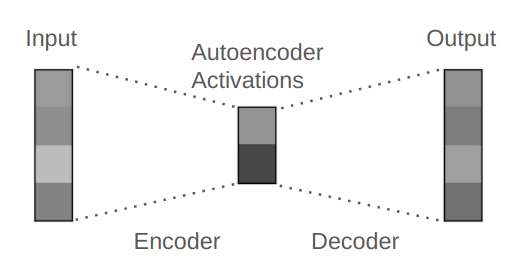
\includegraphics[width=0.5\linewidth]{\toplevelprefix/chapters/chapter5/figs/autoencoder.png}
  \caption{Ilustrarea unui autocodor tipic precum PCA, căutând
  o reprezentare de dimensiune redusă $\bm{z}$ a datelor de dimensiune înaltă $\vx$.}
  \label{fig:AE}
\end{figure}

După cum am văzut în \Cref{ch:classic}, când distribuția lui $\vx$ este într-adevăr
suportată pe un subspațiu de dimensiune redusă $\vU_o$, compactitatea
reprezentării
$\vz$ produsă de $\mathcal{E}$ este o consecință directă a estimării corecte
(și impunerii) dimensiunii acestui subspațiu. În final,
amintiți-vă că coborârea gradientului pe criteriul de reconstrucție produce exact
aceste mapări consistente pe eșantioane: într-adevăr, soluția optimă
la problema
\begin{equation}\label{eq:pca-reconstruction-ch5}
  \min_{\vU^\top \vU = \vI}\, \bE_{\vx}\left[\norm*{\vx
  - \vU\vU^\top \vx}_2^2\right]
\end{equation}
coincide precis cu $\vU_o$ când dimensiunea reprezentării este
suficient de mare. În acest caz, obținem consistența pe eșantioane
gratuit, deoarece aceasta garantează că $\vU_o\vU_o^\top \vx = \vx$.
Observați că în cazul PCA, termenul de reducere a ratei din
\eqref{eqn:autoencode-objective-ch5} devine nul deoarece regularizarea
asupra reprezentării $\Z$ căutate este explicită: Ea acoperă întregul
subspațiu de dimensiune inferioară\footnote{Se poate considera $\Delta R = 0$ în acest caz.}.

\paragraph{PCA Online.} Observați că în construcția de mai sus, transformarea
liniară $\vU$
utilizată pentru codare și decodare este calculată „offline" din toate
datele de intrare în prealabil. O întrebare este dacă această transformare
poate fi învățată „online" pe măsură ce datele de intrare vin în ordine. Această
întrebare a fost răspunsă de lucrarea lui Oja în 1982 \cite{Oja1982SimplifiedNM}.
\begin{example}[Schema de învățare hebbiană normalizată pentru PCA] Considerăm o
  secvență de vectori aleatori i.i.d. $\x_1, \ldots, \x_i, \ldots \in
  \mathbb{R}^n$ cu covarianța $\boldsymbol{\Sigma} \in
  \mathbb{R}^{n\times n}$. Fie $\vu_0 \in \mathbb{R}^n$ și definim
  răspunsul unui vector de intrare $\x_i$ față de un vector de ponderi
  $\vu_i$ ca fiind produsul lor scalar:
  \begin{equation}
    \eta_i = \vu_i^T \x_i
  \end{equation}
  și actualizăm vectorul de ponderi conform următoarei scheme:
  \begin{equation}
    \vu_{i+1} = \frac{\vu_i + \gamma \eta_i \x_i}{\|\vu_i + \gamma
    \eta_i \x_i\|_2}
    \label{eqn:Hebbian}
  \end{equation}
  pentru un câștig mic $\gamma >0$. Această schemă de actualizare poate fi văzută
  ca o schemă hebbiană normalizată, în care ponderile conexiunilor
  dintre neuroni devin mai puternice dacă (produsele) atât intrării
  $\x$ cât și ieșirii $\eta$ sunt puternice. Se poate vedea vectorul de
  ponderi $\vu$ ca fiind „învățat" pe baza unei forme de feedback de la
  ieșirea $\eta$.
  Apoi, în condiții rezonabile, Oja \cite{Oja1982SimplifiedNM} a
  arătat că $\vu_i$ converge către vectorul propriu asociat cu
  cea mai mare valoare proprie a $\boldsymbol{\Sigma}$.
\end{example}

Schema hebbiană normalizată \eqref{eqn:Hebbian} poate fi interpretată ca
o aproximare de ordinul întâi a unei scheme de coborâre a gradientului proiectată
\textit{stocastică} pe
obiectivul problemei \eqref{eq:pca-reconstruction-ch5} (cu dimensiunea lotului
$1$ și cu numărul de coloane ale $\vU$ egal cu $1$) atâta timp cât
$\norm{\vu}_2 = 1$, care este menținută de operația de proiecție din
\eqref{eqn:Hebbian}.
Merită să o păstrăm în minte, atât ca
o dovadă a corectitudinii pentru utilizarea metodelor gradientului stocastic pentru
optimizarea costurilor de reconstrucție precum
\eqref{eq:pca-reconstruction-ch5}, cât și pentru
sugestia sa că \textit{algoritmi mai simpli decât propagarea înapoi
  (de la capăt la capăt) pot
reuși în învățarea autocodorilor consistenți}.

\begin{figure}
  \centering
  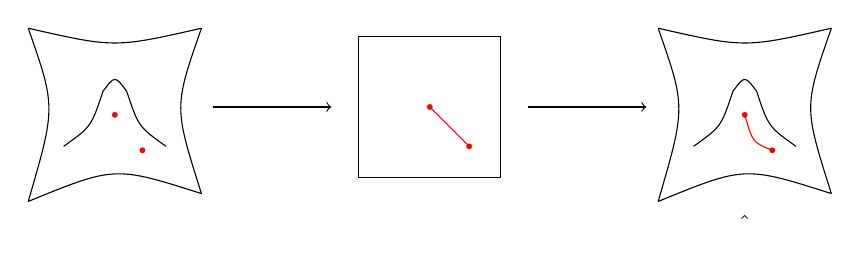
\begin{tikzpicture}
    \draw (-0.1, -0.2) .. controls (1, 0.25) .. (2.1, -0.1);
    \draw (2.1, -0.1) .. controls (1.75, 1) .. (2.1, 2);
    \draw (2.1, 2) .. controls (1, 1.75) .. (-0.1, 2);
    \draw (-0.1, 2) .. controls (0.25, 1) .. (-0.1, -0.2);

    \draw (0.35, 0.5) .. controls (0.7, 0.75) .. (0.85, 1.2);
    \draw (0.85, 1.2) .. controls (1.0, 1.4) .. (1.15, 1.2);
    \draw (1.15, 1.2) .. controls (1.3, 0.75) .. (1.65, 0.5);

    \node[fill, red, circle, inner sep=0.75pt] at (1, 0.9) {};
    \node[fill, red, circle, inner sep=0.75pt] at (1.35, 0.45) {};

    \node at (1, -0.5) {\(\x\)};

    \draw[->] (2.25, 1) -- (3.75, 1);
    \node at (3, 1.25) {\(\fl\)};

    \draw (4.1, 0.1) -- (5.9, 0.1);
    \draw (5.9, 0.1) -- (5.9, 1.9);
    \draw (5.9, 1.9) -- (4.1, 1.9);
    \draw (4.1, 1.9) -- (4.1, 0.1);

    \node[fill, red, circle, inner sep=0.75pt] at (5, 1) {};
    \node[fill, red, circle, inner sep=0.75pt] at (5.5, 0.5) {};

    \draw[red] (5, 1) -- (5.5, 0.5);

    \node at (5, -0.5) {\(\z\)};

    \draw[->] (6.25, 1) -- (7.75, 1);
    \node at (7, 1.25) {\(\re\)};

    \draw (7.9, -0.2) .. controls (9, 0.25) .. (10.1, -0.1);
    \draw (10.1, -0.1) .. controls (9.75, 1) .. (10.1, 2);
    \draw (10.1, 2) .. controls (9, 1.75) .. (7.9, 2);
    \draw (7.9, 2) .. controls (8.25, 1) .. (7.9, -0.2);

    \draw (8.35, 0.5) .. controls (8.7, 0.75) .. (8.85, 1.2);
    \draw (8.85, 1.2) .. controls (9.0, 1.4) .. (9.15, 1.2);
    \draw (9.15, 1.2) .. controls (9.3, 0.75) .. (9.65, 0.5);

    \node[fill, red, circle, inner sep=0.75pt] at (9, 0.9) {};
    \node[fill, red, circle, inner sep=0.75pt] at (9.35, 0.45) {};

    \draw[red] (9, 0.9) .. controls (9.1, 0.55) .. (9.35, 0.45);

    \node at (9, -0.5) {\(\hat{\x}\)};
  \end{tikzpicture}
  \caption{O reprezentare a interpolării prin aplatizarea varietății
    pe o varietate în \(\R^{3}\) de dimensiune \(d = 2\). Pentru a interpola
    două puncte pe varietatea datelor, mapați-le prin harta de aplatizare
    \(\fl\) în spațiul aplatizat, luați interpolanții lor convecși,
    și apoi mapați-i înapoi pe varietatea datelor prin harta de
  reconstrucție \(\re\).}
  \label{fig:idealized_interpolation}
\end{figure}

\subsection{PCA Neliniară și Autocodare}\label{sub:nonlinear-pca}\label{sec:NLPCA}
Desigur, ar trebui să ne așteptăm ca lucrurile să nu mai fie atât de simple
când avem de-a face cu distribuții mai complexe ale căror
structuri de dimensiune redusă de bază sunt neliniare.

\paragraph{Date pe o Subvarietate Neliniară.} Deci, pentru a depăși structura
liniară abordată de PCA, putem presupune că distribuția datelor se află pe o subvarietate (netedă) $\mathcal{M}$. Dimensiunea intrinsecă a subvarietății, să zicem $d$, este de obicei mult mai mică decât
dimensiunea spațiului ambiental $\mathbb{R}^D$. Din această perspectivă
geometrică, de obicei vrem să găsim o mapare neliniară $f$ astfel încât
varietatea rezultată
$f(\mathcal{M})$ să fie aplatizată, așa cum este ilustrat de exemplul arătat în
\Cref{fig:idealized_interpolation}. Spațiul caracteristic $\vz$ rezultat
este de obicei
mai compact (de dimensiune mai mică) decât spațiul $\vx$, iar
varietatea este plată.
Din perspectiva statistică, care este complementară perspectivei geometrice
dar distinctă în general, putem, de asemenea, să vrem să ne asigurăm că distribuția
datelor pe $\mathcal{M}$ este mapată la o distribuție suficient de regulată,
să zicem o distribuție gaussiană sau uniformă (cu
suport de dimensiune foarte redusă), în spațiul $\vz$. Aceste două proprietăți asigură că eșantionarea și interpolarea în spațiul $\vz$ sunt cât mai ușoare posibil, și sunt formalizări matematice ale
noțiunilor dezirabile de caracteristici compacte și structurate în modelul varietății
de dimensiune redusă pentru distribuția datelor.
În general, problema învățării unei astfel de mapări de autocodare pentru această clasă
de distribuții de date este cunoscută ca {\em analiza componentelor principale neliniare}
(NLPCA).

\paragraph{O Încercare Clasică prin Rețea cu Două Straturi.} După cum am
văzut mai sus, în cazul PCA, o rețea neuronală liniară cu un singur
strat este suficientă. Aceasta nu mai este cazul pentru NLPCA. În 1991, Kramer
\cite{Kramer1991NonlinearPC} a propus să rezolve NLPCA folosind o rețea
neuronală cu două straturi pentru a reprezenta maparea codificatorului $f$ (sau inversul său $g$) bazată
pe proprietatea de reprezentare universală a rețelelor cu două straturi cu activare
sigmoidă:
\begin{equation}
  \z = \vW_2 \sigma(\vW_1\x +\vb),
\end{equation}
unde $\sigma(\spcdot)$ este funcția sigmoidă:
\begin{equation}
  \sigma(x) = \frac{1}{1+ e^{-x}}.
\end{equation}
Cybenko \cite{Cybenko1989ApproximationBS} a arătat că funcțiile de
forma de mai sus (cu suficiente noduri ascunse) pot aproxima orice funcție
neliniară netedă, să zicem codificatorul $f(\spcdot)$, cu o precizie
arbitrară. În special, ele pot reprezenta hărțile de aplatizare și reconstrucție
pentru distribuții de date suportate pe uniuni de varietăți de dimensiune redusă,
ca în \Cref{fig:idealized_interpolation}. Arhitectura generală a
rețelelor originale propuse de Kramer este ilustrată în \Cref{fig:NLPCA}.
\begin{figure}[tb]
  \centering
  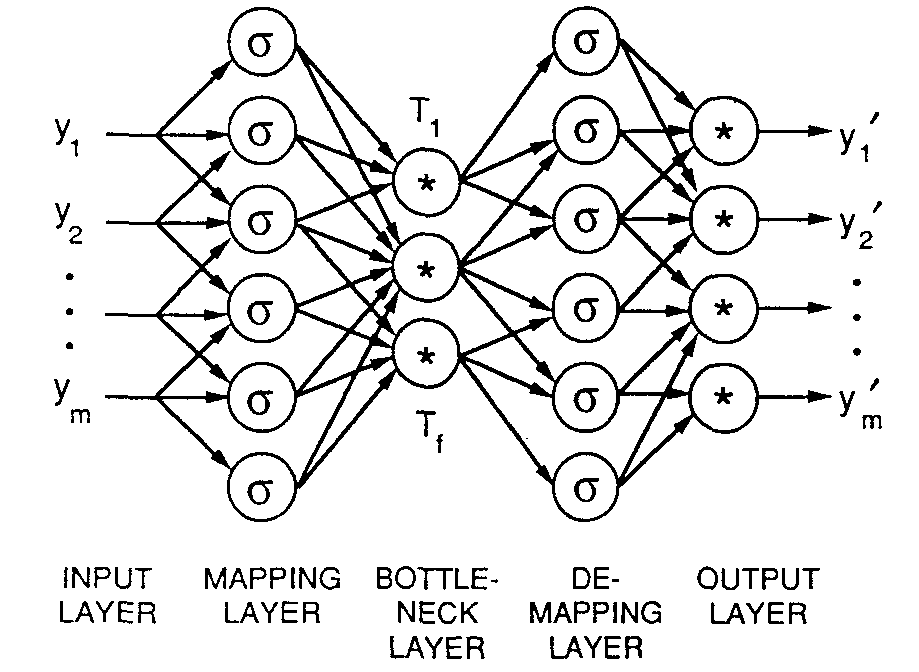
\includegraphics[width=0.6\linewidth]{\toplevelprefix/chapters/chapter5/figs/kramer1991nonlinearPCA.png}
  \caption{PCA neliniară prin rețele neuronale autoasociative de adâncime
    doi atât pentru mapările de codare cât și decodare, sugerată de
  Kramer \cite{Kramer1991NonlinearPC}.}
  \label{fig:NLPCA}
\end{figure}

Din păcate, spre deosebire de cazul PCA de mai sus, nu există în general nicio
schemă de învățare în formă închisă pentru parametrii $\boldsymbol{\theta} =
(\vW, \vb)$ ai acestor rețele. Prin urmare, s-a propus să se antreneze
rețeaua prin propagare înapoi cu supravegherea erorii de reconstrucție:
\begin{equation}\label{eq:nonlinear-pca-ch5}
  \min_{\boldsymbol{\theta}} \mathbb{E}[ \|\x - \hat{\x}(\boldsymbol{\theta})\|_2^2].
\end{equation}
Comparativ cu cazul simplu al PCA, utilizăm același obiectiv de reconstrucție
pentru învățare, dar o clasă mult mai complexă de modele neliniare pentru
parametrizarea și învățarea codificatorului și decodificatorului. Deși proprietățile
de aproximare universală precum cele ale lui Cybenko sugerează că \textit{în principiu}
învățarea autocodorilor consistenți prin acest cadru este posibilă---deoarece pentru
orice eșantion aleator de date, având suficienți parametri, astfel de perechi de autocodare
există---adesea se constată că este foarte netrivial să le găsim folosind coborârea gradientului.
Mai mult, pentru a obține un obiectiv de reconstrucție suficient de informativ
și un model pentru
distribuția datelor de dimensiune înaltă din lumea reală, cum ar fi imaginile, numărul necesar
de eșantioane și noduri ascunse poate fi uriaș.
În plus, ca măsură a compactității reprezentării învățate,
dimensiunea (inferioară) a $\z$ pentru stratul îngust este adesea aleasă
euristic.\footnote{În lucrarea ulterioară \cite{Hinton-1993}, Hinton et al. au sugerat să folosească principiul lungimii minime de descriere (MDL) pentru a promova
  compactitatea schemei de codare învățate, într-un spirit foarte similar cu
măsura ratei de distorsiune introdusă în această carte.}

\paragraph{Aplatizarea Varietății printr-o Rețea Mai Profundă.}
Bazându-ne pe practica modernă a rețelelor profunde, astfel de arhitecturi clasice de rețea
puțin adânci și late sunt cunoscute ca fiind destul de dificil de
antrenat eficient și eficace prin propagare înapoi (BP), parțial
din cauza gradientului care dispare al funcției sigmoide. Prin urmare,
practica modernă sugerează în mod normal să se descompună în continuare
transformarea neliniară $f$ (sau $g$) într-o compoziție de
mai multe straturi de transformări mai simple, rezultând o arhitectură de rețea mai profundă
\cite{Hinton504}, așa cum este ilustrat în \Cref{fig:ccnet_layers}.
În contextul modern, elaborări suplimentare peste costul de reconstrucție de bază
\eqref{eq:nonlinear-pca-ch5} se dovedesc, de asemenea, necesare pentru a obține performanțe bune pe
distribuții de date complexe din lumea reală, cum ar fi imaginile.

\begin{figure}[htb]
  \centering
  \begin{tikzpicture}
    \draw (-0.1, -0.2) .. controls (1, 0.25) .. (2.1, -0.1);
    \draw (2.1, -0.1) .. controls (1.75, 1) .. (2.1, 2);
    \draw (2.1, 2) .. controls (1, 1.75) .. (-0.1, 2);
    \draw (-0.1, 2) .. controls (0.25, 1) .. (-0.1, -0.2);

    \draw (0.35, 0.5) .. controls (0.7, 0.75) .. (0.85, 1.2);
    \draw (0.85, 1.2) .. controls (1.0, 1.4) .. (1.15, 1.2);
    \draw (1.15, 1.2) .. controls (1.3, 0.75) .. (1.65, 0.5);

    \node at (1, -0.5) {\(\x\)};

    \draw[->] (2.25, 1.25) -- (3.25, 1.25);
    \node at (2.75, 1.5) {\(\fl_{1}\)};

    \draw[->] (3.5, 1.25) -- (4.5, 1.25);
    \node at (4, 1.5) {\(\fl_{2}\)};

    \draw[->] (4.75, 1.25) -- (5.75, 1.25);
    \node at (5.25, 1.5) {\(\cdots\)};

    \draw[->] (6, 1.25) -- (7, 1.25);
    \node at (6.5, 1.5) {\(\fl_{L}\)};

    \draw[->] (7, 0.75) -- (6, 0.75);
    \node at (6.5, 0.5) {\(\re_{L}\)};

    \draw[->] (5.75, 0.75) -- (4.75, 0.75);
    \node at (5.25, 0.5) {\(\cdots\)};

    \draw[->] (4.5, 0.75) -- (3.5, 0.75);
    \node at (4, 0.5) {\(\re_{2}\)};

    \draw[->] (3.25, 0.75) -- (2.25, 0.75);
    \node at (2.75, 0.5) {\(\re_{1}\)};

    \draw (7.3, 0.1) -- (9.1, 0.1);
    \draw (9.1, 0.1) -- (9.1, 1.9);
    \draw (9.1, 1.9) -- (7.3, 1.9);
    \draw (7.3, 1.9) -- (7.3, 0.1);

    \node at (8.2, -0.5) {\(\z\)};

  \end{tikzpicture}
  \caption{O reprezentare a procesului de construcție a perechii de aplatizare
    și reconstrucție \((\fl, \re)\), unde codificatorul \(\fl =
    \fl_{L} \circ \fl_{L - 1} \circ \cdots \circ \fl_{1}\) este
    construit din compunerea straturilor de aplatizare, iar decodificatorul \(\re
    = \re_{1} \circ \re_{2} \circ \cdots \circ \re_{L}\) este compus din
  inversiunile fiecărui \(\fl_{\ell}\).}
  \label{fig:ccnet_layers}
\end{figure}

În lumina teoremelor de aproximare universală precum cea a lui Cybenko, cineva
ar putea să se întrebe inițial de ce, conceptual, autocodoarele mai profunde ar trebui să fie preferate
față de cele puțin adânci.
Din perspectiva pur a expresivității, putem înțelege acest fenomen
printr-un unghi geometric legat de sarcina de aplatizare a varietății
neliniare pe care este suportată distribuția noastră ipotezată a datelor. O abordare pur
constructivă pentru aplatizarea varietății procedează incremental, în
paralel cu ceea ce am văzut în \Cref{ch:compression,ch:representation} cu
interacțiunea dintre difuzie, eliminarea zgomotului și compresie. În cadrul geometric,
\textit{procesul de aplatizare} incremental corespunzător lui $f_{\ell}$
ia forma transformării unei vecinătăți a unui punct al varietății pentru a fi
mai aproape de o varietate plată (adică un subspațiu) și impunerea consistenței locale
cu restul eșantioanelor de date; operația incrementală corespunzătoare în
decodificator, $g_{\ell}$, anulează această transformare. Această procedură încorporează precis
informații despre curbură despre varietatea de bază, care este
estimată din eșantioanele de date. Având suficiente eșantioane din varietate și
o instanțiere atentă a acestui proces conceptual, este posibil să se implementeze
această procedură ca o procedură computațională care aplatizează verificabil varietățile
neliniare într-un mod de tip cutie albă \cite{Psenka-JMLR24}. Cu toate acestea, abordarea este
limitată în aplicabilitatea sa la distribuții de date de dimensiune înaltă, cum ar fi
imaginile, din cauza scalabilității nefavorabile, motivând dezvoltarea unor metode
mai flexibile pentru autocodarea incrementală.

\subsection{Autocodare Rară}
În schemele de autocodare de mai sus, dimensiunea spațiului caracteristic
$d$ este de obicei aleasă să fie mult mai mică decât cea a spațiului original de date
$D$ pentru a impune sau promova în mod explicit reprezentarea învățată
să fie de dimensiune redusă. Cu toate acestea, în practică,
în mod normal nu cunoaștem dimensiunea intrinsecă a distribuției
datelor. Prin urmare, alegerea dimensiunii spațiului caracteristic pentru
autocodare se face adesea empiric. În situații mai generale,
distribuția datelor poate fi un amestec de câteva subspații
sau subvarietăți de dimensiune redusă. În aceste cazuri, nu mai este fezabil
să se impună un singur spațiu de dimensiune redusă pentru toate caracteristicile împreună.

Autocodorul rar este menit să rezolve unele dintre aceste limitări. În
particular, dimensiunea spațiului caracteristic poate fi egală cu sau
chiar mai mare decât cea a spațiului datelor, așa cum este ilustrat în
\Cref{fig:SAE}. Cu toate acestea, caracteristicile trebuie să fie foarte
rare în spațiul caracteristic. Deci, dacă impunem raritatea ca măsură
de parsimonie în plus față de reducerea ratei în obiectivul
\eqref{eqn:autoencode-objective-ch5}, obținem un nou obiectiv pentru
autocodarea rară:
\begin{equation}
  \min_{f, g}
  [\|\Z\|_0 - \Delta R_{\epsilon}(\Z) + d(\X, \hat \X)],
  \label{eqn:autoencode-sparse}
\end{equation}
unde „norma" $\ell^0$ $\|\spcdot\|_0$ este cunoscută pentru a promova raritatea.
Aceasta este foarte similară cu obiectivul de reducere a ratei rare
\eqref{eq:sparse-rr} pe care l-am folosit în \Cref{ch:representation} anterior pentru a deriva arhitectura CRATE de tip cutie albă.

\begin{figure}
  \centering
  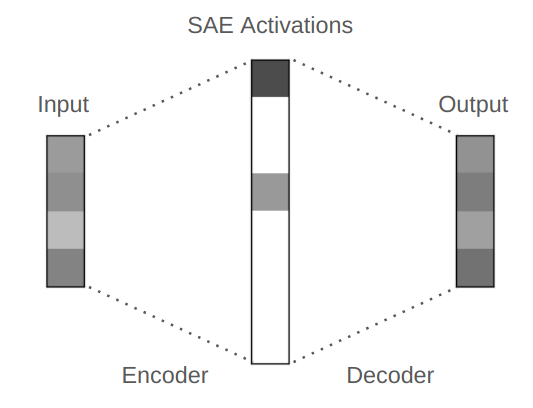
\includegraphics[width=0.5\linewidth]{\toplevelprefix/chapters/chapter5/figs/SAE_diagram.png}
  \caption{Ilustrarea unui autocodor rar (SAE), comparat cu
  cel al unui autocodor tipic (AE) din \Cref{fig:AE}. }
  \label{fig:SAE}
\end{figure}


Ca metodă pentru învățarea perechilor de autocodare într-un mod de la capăt la capăt, autocodarea
rară a fost practicată în trecut
\cite{Ranzato2006-oq,10.5555/3042573.3042641}, dar aproape toate cadrele moderne
de autocodare se bazează în schimb pe un cadru diferit, probabilistic
de autocodare, pe care îl vom studia acum.

\subsection{Autocodare Variațională}\label{sec:vae}

În concepția clasică a autocodării, urmând Hinton și Rumelhart
\cite{Rumelhart1986}, distribuția datelor joacă un rol foarte minor în
formulare, în ciuda centralității sale pentru reprezentarea pe care o
învățăm în cele din urmă. Într-adevăr, în cadrul naiv, se speră că prin antrenarea unei rețele profunde
pentru a reconstrui eșantioane din distribuția datelor cu un gât de sticlă configurabil
corespunzător pentru reprezentarea $\vz$, codificatorii învățați $f$ și $g$ vor
ajunge în mod natural să corespundă unei reprezentări de caracteristici
compacte și structurate pentru date. Acest lucru este rareori cazul în practică.
O metodologie îmbunătățită, mai modernă pentru autocodare care încă găsește
aplicații semnificative până în prezent este \textit{autocodarea variațională}
\cite{Kingma2013-sb,Kingma2019-zh}.
Vom vedea cum acest cadru, care antrenează un autocodor variațional (VAE)
derivat prin considerații de modelare probabilistică, atât generalizează
antrenamentul clasic al autocodorului (prin minimizarea pierderii de reconstrucție),
cât și îl stabilizează cu regularizare adecvată. Mai târziu, vom vedea cum să
mergem mai departe și să depășim natura de tip cutie neagră a rețelelor profunde folosite
pentru a reprezenta mapările de codare și decodare $f$ și $g$.

\subsubsection{Perspectiva Probabilistică asupra Autocodării}
În modelul varietății pentru distribuția datelor, obiectele matematice cheie
sunt \textit{suportul} distribuției datelor, și anume varietatea $\cM$,
și densitatea datelor pe suport, să zicem $p$. Când formulăm
autocodarea din perspectiva probabilistică, adesea ne gândim la
intrarea de dimensiune înaltă $\vx$ ca având o densitate $p$ cu suport pe $\R^D$; se
poate gândi la adăugarea unei cantități foarte mici de zgomot la distribuția (degenerată)
suportată pe varietatea $\cM$ pentru a obține această densitate $p$, în linie
cu construcțiile noastre de eliminare a zgomotului-difuzie din \Cref{ch:compression}.
Apoi obiectivul modelării probabilistice generative este să învețe densitatea $p$
din eșantioane $\vx$, să zicem dintr-o clasă de modele $p(\vx;\, \vtheta)$ parametrizate
de $\vtheta$. După cum am reamintit în \Cref{ch:compression}, o abordare clasică
pentru a realiza acest lucru este prin estimarea maximei verosimilități:
\begin{equation*}\label{eq:VAE-MLE}
\max_{\vtheta}\, \bE_{\vx}[ \log p(\vx;\, \vtheta) ].
\end{equation*}
Pentru anumite clase reprezentative de distribuții de date $p$
și clase suficient de expresive de modele $p(\vx;\, \vtheta)$, chiar și probleme
de învățare mai simple decât estimarea maximei verosimilități sunt cunoscute ca fiind
statistic dificile \cite{Yang1999-wb}. Prin urmare, este de dorit să exploatăm
cunoașterea că $\vx$ are structură de dimensiune redusă căutând să factorizăm
distribuția $p(\vx ;\, \vtheta)$ conform unui model de variabilă „latentă"
de dimensiune redusă $\vz$. Într-adevăr, prin condiționare putem scrie $p(\vx,
\vz ;\, \vtheta)
= p(\vz;\, \vtheta) p(\vx \mid \vz;\, \vtheta)$, și
\begin{align*}
p(\vx; \vtheta) &= \int p(\vz;\, \vtheta) p(\vx \mid \vz;\, \vtheta) \odif \vz
\\
&=
\bE_{\vz \sim p(\,\cdot\,;\, \vtheta)}[ p(\vx \mid \vz;\, \vtheta) ].
\end{align*}
Clasic, modelul nostru pentru distribuția datelor $p(\vx;\, \vtheta)$ corespunde
unei alegeri a distribuției latente $p(\vz;\, \vtheta)$ și a distribuției
condiționale $p(\vx \mid \vz;\, \vtheta)$.
Chiar și așa, calcularea modelului pentru distribuția datelor din aceste distribuții
latente este intractabilă, cu excepția cazurilor speciale, analoge celor pe care le-am
studiat în \Cref{ch:classic}.
În același mod, calcularea posteriorului $p(\vz \mid \vx;\, \vtheta)$ din
date, permițându-ne să \textit{codăm} eșantioane la latenții lor corespunzători, este
în general intractabilă.
Există astfel un compromis între expresivitatea modelului nostru generativ,
tractabilitatea sa computațională și acuratețea oricăror aproximări pe care le facem
la cadrul probabilistic de bază de dragul
tractabilității computaționale.
În navigarea acestui compromis, este nevoie și de o abordare computațională flexibilă
pentru învățarea parametrilor modelului $\vtheta$ din date, analogă obiectivului
maximei verosimilități.

În cadrul autocodării variaționale, navigăm acest compromis prin
trei perspective cheie:
\begin{enumerate}
\item Postulăm distribuții \textit{simple} pentru $\vz$ și $\vx$ condiționale
  pe $\vz$, dar facem ca parametrii lor să depindă într-un mod foarte flexibil de
  datele de intrare $\vx$ (unde este relevant) folosind rețele profunde.
\item Înlocuim posteriorul $p(\vz \mid \vx;\, \vtheta)$, folosit pentru codare
  și a cărui formă este implicată (prin regula lui Bayes) de alegerile noastre de modelare pentru $\vz$,
  cu o aproximare tractabilă $q(\vz \mid \vx;\, \veta)$, care are proprii săi
  parametri $\veta$.
\item Învățăm împreună $\vtheta$ și $\veta$ prin maximizarea unei limite inferioare tractabile
  pentru verosimilitatea $p(\vx ;\, \vtheta)$, cunoscută ca limita inferioară a dovezilor (ELBO).
\end{enumerate}
Ne vom concentra pe instanțierea cea mai utilă a cadrului VAE
în practică, și anume
unde priorul $p(\vz ;\, \vtheta)$ și condiționala $p(\vx \mid \vz;\,
\vtheta)$ sunt ambele gaussiene. Și anume, folosim următoarele distribuții
gaussiene:
\begin{align*}
\vz &\sim \cN(\Zero, \vI), \\
\vx \mid \vz &\sim \cN(g_1(\vz), \diag(e^{g_2(\vz)}) \vI),
\end{align*}
unde $g = (g_1, g_2)$ sunt rețele profunde cu parametrii $\vtheta$, care
corespund \textit{decodificatorului} în autocodor.
Similar, pentru posteriorul aproximativ $q(\vz \mid \vx;\, \veta)$, folosim
o distribuție gaussiană specială cu parametri dați de un codificator
MLP $f = (f_1, f_2)$ cu parametrii $\veta$:
\begin{equation*}
\vz \mid \vx \sim \cN(f_1(\vx), \diag(e^{f_2(\vx)}) \vI).
\end{equation*}
Aceasta face codarea și decodarea probabilistică simple: pur și simplu mapăm datele noastre
$\vx$ la parametrii de medie și varianță ai unei distribuții gaussiene pentru
codare, și viceversa pentru decodare.
Pentru învățarea codificatorului și decodificatorului, pornim de la obiectivul
maximei verosimilități \Cref{eq:VAE-MLE} și derivăm o limită inferioară convenabilă cunoscută ca
limita inferioară a dovezilor, sau ELBO. Pornind de la manipulări algebrice simple
\begin{align*}
\log p(\vx;\, \vtheta) &=
\log \frac{p(\vx, \vz;\, \vtheta)}{p(\vz \mid \vx;\, \vtheta)}
\\
&=
\log \frac{p(\vx, \vz;\, \vtheta)}{q(\vz \mid \vx;\, \veta)}
+
\log \frac{q(\vz \mid \vx;\, \veta)}{p(\vz \mid \vx;\, \vtheta)},
\end{align*}
luăm așteptări în raport cu $\vz \sim q(\,\cdot\, \mid
\vx;\, \veta)$ și
folosim inegalitatea Gibbs (\Cref{thm:information-inequality}) pentru a obține
\begin{equation*}
\log p(\vx;\, \vtheta)
\geq
\bE_{\vz \sim q(\,\cdot\, \mid \vx ;\, \veta)} \left[
  \log \frac{p(\vx, \vz;\, \vtheta)}{q(\vz \mid \vx;\, \veta)}
\right].
\end{equation*}
Partea dreaptă a acestei limite este ELBO; ca limită inferioară pentru log-verosimilitatea
punctuală a $p(\vx;\, \vtheta)$, maximizarea sa oferă un compromis
principial
între obiectivul maximei verosimilități și tractabilitatea computațională.
Interesant, derivarea de mai sus arată că strânsoarea sa depinde de divergența
KL între posteriorul aproximativ $q(\vz \mid \vx;\, \veta)$ și
posteriorul adevărat $p(\vz \mid \vx;\, \vtheta)$, implicând că cu cât posteriorul nostru
aproximativ este mai precis, cu atât maximizarea ELBO conduce la
maximizarea obiectivului de bază de interes, verosimilitatea
datelor. Astfel, obiectivul VAE este:
\begin{equation}\label{eq:elbo-objective}
\max_{\vtheta, \veta}\,
\bE_{\vx}
\bE_{\vz \sim q(\,\cdot\, \mid \vx ;\, \veta)} \left[
  \log \frac{p(\vx, \vz;\, \vtheta)}{q(\vz \mid \vx;\, \veta)}
\right].
\end{equation}
Prin derivarea noastră, maximizarea acestui obiectiv corespunde unui compromis
între maximizarea funcției de verosimilitate a datelor și minimizarea divergenței
KL între posteriorul aproximativ și cel adevărat, care este un obiectiv foarte
sensibil având în vedere ipotezele de modelare VAE.

\subsubsection{Antrenarea VAE ca Autocodare Probabilistică}

Există o metodologie generală pentru maximizarea obiectivului ELBO din
\Cref{eq:elbo-objective} folosind coborârea gradientului stocastic și diverși estimatori
Monte Carlo tractabili pentru gradienții asociați. Cu toate acestea, sarcina este
mai simplă sub ipotezele gaussiene pe care le-am făcut mai sus. În acest caz, ELBO
citește
\begin{align*}
&\max_{\vtheta, \veta}\,
\bE_{\vx}
\bE_{\vz \sim q(\,\cdot\, \mid \vx ;\, \veta)} \left[
  \log \frac{p(\vx, \vz;\, \vtheta)}{q(\vz \mid \vx;\, \veta)}
\right]\\
=&
\max_{\vtheta, \veta}\,
\left\{
  \bE_{\vx}
  \bE_{\vz \sim q(\,\cdot\, \mid \vx ;\, \veta)} \left[
    \log p(\vx, \vz;\, \vtheta)
  \right]
  + \frac{d \log(2\pi e)}{2}
  + \frac{1}{2} \ip{ \bE_{\vx}[f_2(\vx)]}{\mathbf{1}}
\right\}
\\
\equiv &
\max_{\vtheta, \veta}\,
\left\{
  \bE_{\vx}
  \bE_{\vz \sim q(\,\cdot\, \mid \vx ;\, \veta)} \left[
    \log p(\vx \mid \vz;\, \vtheta)
    + \log p(\vz)
  \right]
  + \frac{1}{2} \ip{ \bE_{\vx}[f_2(\vx)]}{\mathbf{1}}
\right\}
\\
\equiv &
\max_{\vtheta, \veta}\,
\left\{
  2\bE_{\vx}\left[
    \bE_{\vz \sim q(\,\cdot\, \mid \vx ;\, \veta)} \left[
      \log p(\vx \mid \vz;\, \vtheta)
    \right]
    + \ip{ f_2(\vx) - e^{f_2(\vx)}}{\mathbf{1}}
    - \norm{f_1(\vx)}_2^2
  \right]
\right\}, \labelthis \label{eq:elbo-for-gaussians}
\end{align*}
urmând \Cref{thm:max_entropy} și calculul entropiei gaussiene realizat în \Cref{app:diffusion-denoising}, unde $\equiv$
denotă echivalența obiectivelor de optimizare (în fiecare caz, eliminăm unele
constante aditive care nu schimbă soluțiile problemei de optimizare).
Termenul rămas corespunde părții de „autocodare" a obiectivului
ELBO: intuitiv, caută să maximizeze verosimilitatea datelor generate de
decodificator când latenții $\vz$ sunt distribuiți conform posteriorului
aproximativ (generat de codificatorul aplicat unui eșantion de date $\vx$), care este
o formă probabilistică de autocodare.
Pentru a vedea acest lucru mai direct, considerați cazul special în care posteriorul
aproximativ se concentrează pe media sa $f_1(\vx)$, pentru fiecare $\vx$: acesta
este limita
unde log-varianța sa $f_{2,i}(\vx) \to -\infty$ pentru fiecare coordonată
$i = 1, \dots, d$.
Pentru simplitate, presupunem mai mult că $g_2(\vx) = \mathbf{1}$, dând decodificatorului
varianță unitară constantă pe fiecare coordonată.
Apoi termenul de pierdere în cauză converge la
\begin{align*}
\bE_{\vx}
\bE_{\vz \sim q(\,\cdot\, \mid \vx ;\, \veta)} \left[
  \log p(\vx \mid \vz;\, \vtheta)
\right]
&\to
\bE_{\vx} \left[
  \log p(\vx \mid f_1(\vx);\, \vtheta)
\right]
\\
&\equiv
-\frac{1}{2} \bE_{\vx} \left[
  \|\vx - g_1\circ f_1(\vx)\|_2^2
\right].
\end{align*}
Deci cu un codificator foarte încrezător, care mapează determinist fiecare eșantion
$\vx$ la un singur punct $f_1(\vx)$ în spațiul $\vz$, și un decodificator izotrop,
partea de „autocodare" a problemei de maximizare ELBO devine într-adevăr
un obiectiv clasic de autocodare!\footnote{În cazul general în care $g_2$ nu este
fixat ca $\mathbf{1}$, cititorul poate verifica că termenul de autocodare din
obiectivul ELBO converge la un obiectiv clasic de autocodare \textit{regularizat}.}
În același timp, observați că acest caz special este de fapt exclus de
termenii suplimentari din \Cref{eq:elbo-for-gaussians}---aceștia corespund efectiv
termenilor de regularizare care descurajează codificatorul să colapseze.
Pierderea generală ELBO (\Cref{eq:elbo-objective,eq:elbo-for-gaussians}) este
prin urmare o generalizare strictă a obiectivului clasic de reconstrucție prin autocodare
(\Cref{eq:nonlinear-pca-ch5}), atât în termenii termenului său de fidelitate a datelor
cât și în termenii includerii termenilor de regularizare.

\subsubsection{Antrenarea unui VAE}
VAE-urile sunt de obicei antrenate prin alternarea ascensiunii gradientului stocastic pe obiectivul
ELBO (\Cref{eq:elbo-for-gaussians}), date fiind eșantioane individuale
$\vx$ din
distribuția adevărată a datelor și din $\vz \sim q(\,\cdot\,\mid \vx;\, \veta)$. În
particular, este standard să se colecteze și să se antreneze pe multe eșantioane generate independent
$\vz^{i}$ pentru fiecare eșantion $\vx$. Pentru a lua gradienți ai
\Cref{eq:elbo-for-gaussians} în raport cu parametrii codificatorului $\veta$,
se folosește așa-numitul truc de reparametrizare scriind $\vz \sim
q(\,\cdot\,\mid \vx;\, \veta)$ ca
\begin{equation*}
\vz =_{\mathrm{d}} f_1(\vx) + \diag(e^{\tfrac{1}{2}f_2(\vx)}) \vg,
\quad \vg \sim
\cN(0, \vI),
\end{equation*}
unde $=_{\mathrm{d}}$ denotă egalitatea în distribuție. Apoi se pot lua pur și simplu
multe eșantioane gaussiene standard independente $\vg^{i}$ pentru fiecare eșantion de date
$\vx$, se generează eșantioanele corespunzătoare din posteriorul aproximativ
$\vz^i$ și se calculează gradienții în raport cu $\veta$ folosind diferențierea
automată fără probleme.



\section{Învățarea Reprezentărilor Auto-Consistente}
\label{sec:self-consistency}

În capitolele anterioare, am studiat metode care ne-ar permite să învățăm o distribuție de dimensiune redusă prin compresie (cu pierderi). După cum am menționat în \Cref{ch:intro} și am demonstrat în capitolele anterioare, progresele făcute în inteligența mașinilor se bazează în mare parte pe găsirea de soluții computațional fezabile și eficiente pentru a realiza compresia dorită, nu doar calculabile sau tractabile în teorie, ci și scalabile în practică:
\begin{equation}
\mbox{\textbf{calculabil}} \;
   \Longrightarrow \; \mbox{\textbf{tractabil}} \; \Longrightarrow \;
   \mbox{\textbf{scalabil}}.
\end{equation}
Este chiar corect să spunem că progresul extraordinar în inteligența mașinilor făcut în ultimul deceniu sau cam așa ceva este în mare parte atribuit dezvoltării modelelor și metodelor scalabile, să zicem prin antrenarea rețelelor profunde prin propagare înapoi. Modele mari cu miliarde de parametri antrenate cu trilioane de puncte de date pe zeci de mii de GPU-uri puternice au demonstrat capacități supra-umane în memorarea cunoștințelor existente. Acest lucru i-a determinat pe mulți să creadă că „inteligența" acestor modele va continua să se îmbunătățească pe măsură ce scala lor continuă să crească.

În timp ce sărbătorim minunile inginerești ale unor astfel de sisteme mari de învățare automată create de om, trebuie să admitem și că, în comparație cu inteligența din natură, această abordare pentru îmbunătățirea inteligenței mașinilor necesită resurse în mod inutil de multe. Ființele inteligente naturale, inclusiv animalele și oamenii, pur și simplu nu își pot permite o astfel de soluție de forță brută pentru învățare deoarece trebuie să opereze cu un buget foarte limitat în energie, spațiu și timp, supuse multor constrângeri fizice stricte.

În primul rând, există dovezi științifice puternice că creierul nostru nu efectuează propagare înapoi globală de la capăt la capăt pentru a-și îmbunătăți sau corecta predicțiile. În schimb, este cunoscut de mult timp în neuroștiință că creierul nostru corectează erorile cu feedback local în buclă închisă, cum ar fi codarea predictivă. Aceasta a fost baza științifică care l-a inspirat pe Norbert Wiener să dezvolte teoria controlului prin feedback și programul Ciberneticii în anii 1940.

În al doilea rând, am văzut în secțiunile anterioare că pentru a învăța o reprezentare consistentă, trebuie să învățăm o autocodare bidirecțională:
\begin{equation}
 \X
\xrightarrow{\hspace{1mm} \mathcal{E} = f \hspace{1mm}} \Z  \xrightarrow{\hspace{1mm} \mathcal{D} = g \hspace{1mm}} \hat{\X}.
\end{equation}
Aceasta necesită impunerea ca datele de intrare observate $\X$ și cele decodate $\hat \X$ să fie apropiate printr-o anumită măsură de similaritate $d(\X, \hat \X)$. În natură, animalele sau oamenii rareori au acces direct la adevărul de bază $\X$. De exemplu, nu avem niciodată acces direct la forma 3D adevărată, distanța sau dinamica obiectelor dintr-o scenă. Cu toate acestea, toți am învățat să le estimăm și să le prezicem foarte precis și eficient. Prin urmare, o întrebare importantă este: cum putem învăța distribuția adevărată a $\X$, chiar dacă nu putem compara direct estimarea noastră $\hat \x$ cu adevărul de bază $\x$? După cum vom vedea în acest capitol, răspunsul constă, de asemenea, în feedback-ul în buclă închisă, precum și în dimensionalitatea redusă a distribuției datelor.






După cum știm din capitolul anterior, pentru a ne asigura că o reprezentare este consistentă, trebuie să comparăm $\hat \X \sim p(\hat\x)$ generat și $\X \sim p(\x)$ original, cel puțin în distribuție. Chiar și când avem acces la $\X$ și $\hat \X$, tehnic, calcularea și minimizarea distanței dintre două distribuții poate fi problematică, mai ales când suportul distribuțiilor este de dimensiune redusă. Divergența KL introdusă în \Cref{ch:compression} nu este nici măcar bine definită între două distribuții care nu au suporturi suprapuse.

Ca o încercare timpurie de a atenua dificultatea de mai sus în calcularea și minimizarea distanței dintre două distribuții (de dimensiune redusă), oamenii au sugerat învățarea generatorului/decodificatorului $g$ prin abordări discriminative \cite{Tu-2007}. Această linie de gândire a condus la ideea de {\em Rețele Generative Adversariale (GAN)} \cite{goodfellow2014generative}. Aceasta introduce un discriminator $d$, de obicei modelat de o rețea profundă, pentru a discerne diferențele dintre eșantioanele generate $\hat \X$ și cele reale $\X$:
\begin{equation}
 \Z \xrightarrow{\hspace{2mm} g(\z,\eta) \hspace{2mm}} \hat \X, \, \X \xrightarrow{\hspace{2mm} d(\x, \theta)\hspace{2mm}} \{\mathbf 0, \mathbf 1\}.
 \label{eqn:GAN}
\end{equation}
Se sugerează că putem încerca să aliniem distribuțiile dintre $\hat \x$ și $\x$ printr-un {\em joc Stackelberg} între generator $g$ și discriminator $d$:
\begin{equation}
\max_{\theta}\min_{\eta} \mathbb{E}_{p({\x})}\big[\log d(\x,\theta)\big] + \mathbb{E}_{p({\z})}\big[1 - \log d(\underbrace{g(\z,\eta)}_{\hat \x \,\sim\, p_g},\theta)\big].
\end{equation}
Adică, discriminatorul $d$ încearcă să minimizeze entropia încrucișată dintre eșantioanele adevărate $\X$ și cele generate $\hat \X$ în timp ce generatorul $g$ încearcă să facă opusul.

Se poate arăta că găsirea unui echilibru pentru jocul Stackelberg de mai sus este echivalentă cu minimizarea {\em divergenței Jensen-Shannon}:
\begin{equation}
    \mathcal{D}_{JS}(p(\x), p_g(\hat \x)) = \mathcal{D}_{KL}\big(p \| (p + p_g)/{2}\big) + \mathcal{D}_{KL}\big(p_g \| (p + p_g)/{2}\big).
\end{equation}
Observați că, în comparație cu divergența KL, divergența JS este bine definită chiar dacă suporturile celor două distribuții nu se suprapun. Cu toate acestea, divergența JS nu are o expresie în formă închisă nici măcar între două gaussiene, în timp ce divergența KL are. În plus, deoarece distribuțiile datelor sunt de dimensiune redusă, divergența JS poate fi foarte slab condiționată pentru optimizare.\footnote{așa cum este arătat în \cite{arjovsky2017wasserstein}.} Acest lucru poate explica de ce multe euristici suplimentare sunt de obicei folosite în multe variante ulterioare ale GAN.

Deci, în schimb, s-a sugerat și înlocuirea divergenței JS cu distanța de mișcare a pământului (EM) sau distanța Wasserstein.\footnote{În linii mari, pentru distribuții cu suporturi de dimensiune redusă potențial nesuprapuse, divergența JS se comportă ca norma $\ell^0$, iar distanța EM se comportă ca norma $\ell^1$.} Cu toate acestea, atât divergența JS cât și distanța Wasserstein pot fi calculate doar aproximativ între două distribuții generale.\footnote{De exemplu, distanța Wasserstein necesită calcularea diferenței maxime între așteptările celor două distribuții peste toate funcțiile 1-Lipschitz.} Mai mult, nici divergența JS nici distanța Wasserstein nu au formule în formă închisă, chiar pentru distribuții gaussiene.\footnote{Distanța Wasserstein (normă $\ell^1$) poate fi mărginită de distanța Wasserstein (normă $\ell^2$) care are o formă închisă \cite{salmona2021gromovwasserstein}. Cu toate acestea, după cum este bine cunoscut în geometria de dimensiune înaltă, norma $\ell^1$ și norma $\ell^2$ deviază semnificativ în termenii proprietăților lor geometrice și statistice pe măsură ce dimensiunea devine mare \cite{Wright-Ma-2021}. Marginea poate deveni foarte slabă.}

Dacă este dificil să comparăm distribuțiile datelor $\X$ și $\hat \X$, ar fi posibil să comparăm caracteristica învățată $\Z$ cu imaginea sa $\hat \Z$ sub codificatorul $f$:
\begin{equation}
 \X
\xrightarrow{\hspace{1mm} \mathcal{E} = f \hspace{1mm}} \Z  \xrightarrow{\hspace{1mm} \mathcal{D} = g \hspace{1mm}} \hat{\X} \xrightarrow{\hspace{1mm} \mathcal{E} = f \hspace{1mm}} \hat \Z?
\label{eqn:closed-autoencoding}
\end{equation}
Aceasta conduce la noțiunea de {\em reprezentare auto-consistentă}.
\begin{definition}[Reprezentare Auto-Consistentă]\label{def:closed_loop}
    Date fiind datele \(\vX\), numim \textit{reprezentare auto-consistentă} o pereche de funcții \((f \colon \cX \to \cZ, g \colon \cZ \to \cX)\), astfel încât \textit{caracteristicile} \(\vZ = f(\vX)\) sunt compacte și structurate, iar \textit{caracteristicile de autocodare} \(\hat{\vZ} \doteq f \circ g(\vZ)\) sunt \textit{apropiate} de \(\vZ\).
    \begin{enumerate}
        \item Spunem că este \textit{auto-consistentă pe eșantioane} dacă \(\vZ \approx \hat{\vZ}\) într-o anumită normă cu probabilitate mare.
        \item Spunem că reprezentarea este \textit{auto-consistentă distributional} dacă \(\Law(\vZ) \approx \Law(\hat{\vZ})\).
    \end{enumerate}
\end{definition}



\subsection{Transcriere în Buclă Închisă prin Jocuri Stackelberg}\label{sec:closed-loop-transcription}



Cum încercăm să ne asigurăm că o reprezentare învățată este auto-consistentă? Ca de obicei, să presupunem $\X = \cup_{k=1}^K \X_k$ cu fiecare subset de eșantioane $\X_k$ aparținând unei subvarietăți de dimensiune redusă: $\X_k \subset \mathcal{M}_k, k = 1,\ldots, K$. Urmând notația din \Cref{ch:general-distribution}, folosim o matrice $\bm \Pi_k(i,i) = 1$ pentru a denota apartenența eșantionului $i$ la clasa $k$ și $\bm \Pi_k(i,j) = 0$ altfel. Se caută o mapare continuă $f(\cdot,\bm \theta): \x \mapsto \z$ de la $\X$ la o reprezentare optimă $\Z = [\z_1, \ldots, \z_N] \subset \mathbb{R}^{d \times N}$:
\begin{equation}
\bm X  \xrightarrow{\hspace{2mm} f(\x, \bm \theta) \hspace{2mm}} \bm Z,
\label{eqn:LDR}
\end{equation}
care maximizează următorul obiectiv de reducere a ratei de codare (MCR$^2$):
\begin{equation}\label{eq:mcr2-formulation}
\begin{split}
\max_{\Z} \; \Delta R_\epsilon(\Z  \mid \bm{\Pi}) %
&\doteq \underbrace{\frac{1}{2}\log\det \Big(\I + {\alpha} \Z \Z^\top \Big)}_{R_{\epsilon}(\Z)} \;-\; \underbrace{\sum_{k=1}^{K}\frac{\gamma_k}{2} \log\det\Big(\I + {\alpha_k} \Z \bm{\Pi}^{j} \Z^\top \Big)}_{R^c_{\epsilon}(\Z \mid \bm \Pi)},
\end{split}
\end{equation}
unde $\alpha = {d}/({N\epsilon^2})$, $\alpha_k = d/({\mathrm{tr}(\bm{\Pi}_k)\epsilon^2})$, $\gamma_k =  {\mathrm{tr}(\bm{\Pi}_{k})}/{N}$ pentru fiecare $k = 1,\dots, K$.

O problemă cu învățarea unei astfel de mapări unilaterale \eqref{eqn:LDR} prin maximizarea obiectivului de mai sus \eqref{eq:mcr2-formulation} este că tinde să extindă dimensiunea subspațiului învățat pentru caracteristicile din fiecare clasă\footnote{Dacă dimensiunea spațiului caracteristic $d$ este prea mare, maximizarea reducerii ratei poate supraestima dimensiunea fiecărei clase. Prin urmare, pentru a învăța o reprezentare bună, trebuie să se preselecteze o dimensiune adecvată pentru spațiul caracteristic, așa cum s-a realizat în experimentele din \cite{yu2020learning}. De fapt, aceeași problemă de „selecție a modelului" persistă chiar și în cel mai simplu caz cu un singur subspațiu, care este PCA clasic \cite{Jolliffe1986}. După cunoștințele noastre, selectarea numărului corect de componente principale într-o situație eterogenă zgomotoasă rămâne un subiect activ de cercetare \cite{hong2020selecting}.}, așa cum am văzut în \Cref{sec:chap4-representation-learning-problem} din \Cref{ch:compression}. Pentru a verifica dacă caracteristicile învățate sunt consistente, adică nici nu supraestimează nici nu subestimează structura intrinsecă a datelor, putem lua în considerare învățarea unui decodificator $g(\cdot,\eta): \z \mapsto  \x$ de la reprezentarea $\Z = f(\X,\bm\theta)$ înapoi la spațiul datelor $\x$: $\hat \X = g(\Z, \bm\eta)$:
\begin{equation}
    \X \xrightarrow{\hspace{2mm} f(\x, \bm\theta)\hspace{2mm}} \Z \xrightarrow{\hspace{2mm} g(\z, \bm \eta) \hspace{2mm}} \hat \X,
    \label{eqn:autoencoding-ch6}
\end{equation}
și verificăm cât de apropiate sunt $\X$ și $\hat \X$. Aceasta formează o autocodare care este ceea ce am studiat extensiv în \Cref{ch:autoencoding} anterior.

\paragraph{Măsurarea distanței în spațiul caracteristic.}
Cu toate acestea, după cum am discutat mai sus, dacă nu avem opțiunea de a calcula distanța dintre $\X$ și $\hat \X$, suntem lăsați cu opțiunea de a compara caracteristicile lor corespunzătoare $\Z$ și $\hat \Z = f(\hat \X, \bm \theta)$. Observați că sub obiectivul MCR$^2$, distribuțiile $\Z$ sau $\hat \Z$ rezultate tind să fie liniare pe bucăți, astfel încât distanța lor poate fi calculată mai ușor. Mai precis, deoarece caracteristicile fiecărei clase, $\Z_k$ și $\hat{\Z}_k$, sunt aproape de a fi un subspațiu/gaussian de dimensiune redusă, „distanța" lor poate fi măsurată prin reducerea ratei, cu \eqref{eq:mcr2-formulation} restricționată la două seturi de dimensiune egală:
\begin{equation}
\Delta R_\epsilon\big(\Z_k, \hat{\Z}_k\big) \doteq R_\epsilon\big(\Z_k \cup \hat{\Z}_k\big) - \frac{1}{2} \big( R_\epsilon\big(\Z_k) + R_\epsilon\big(\hat \Z_k)\big).
\end{equation}
Distanța totală dintre $\Z$ și $\hat \Z$ este dată de:
\begin{equation}
d(\Z, \hat \Z) \doteq   \sum_{k=1}^K \Delta R_\epsilon\big(\Z_k, \hat{\Z}_k\big) =  \sum_{k=1}^K \Delta R_\epsilon\big(\Z_k, f(g(\Z_k, \bm\eta),\bm \theta)\big).
\label{eqn:Z-distance}
\end{equation}


Dacă suntem interesați să discernem {\em orice} diferențe în distribuțiile datelor originale $\X$ și cele decodate $\hat \X$, putem vedea codificatorul de caracteristici $f(\cdot, \bm \theta)$ ca un „discriminator" pentru a {\em mări} orice diferență între toate perechile de $\X_k$ și $\hat \X_k$, prin simpla maximizare a distanței $d(\X, \hat \X)$:
\begin{equation}
\max_f d(\Z, \hat \Z) = \max_{\bm \theta} \sum_{k=1}^K \Delta R_\epsilon\big(\Z_k, \hat{\Z}_k\big) = \max_{\bm \theta} \sum_{k=1}^K \Delta R_\epsilon\big(f(\X_k,\bm \theta), f(\hat{\X}_k,\bm \theta)\big).
    \label{eqn:max-distance}
\end{equation}
Adică, o „distanță" între $\X$ și $\hat \X$ poate fi măsurată ca reducerea maximă realizabilă a ratei între toate perechile de clase din aceste două seturi. Într-un fel, aceasta măsoară cât de bine sau prost se aliniază $\hat \X$ decodat cu datele originale $\X$---prin urmare măsurând calitatea „injectivității" codificatorului $f$. Observați că o astfel de măsură discriminativă este consistentă cu ideea GAN \eqref{eqn:GAN} care încearcă să separe $\X$ și $\hat \X$ în două clase, măsurate prin entropia încrucișată.

Cu toate acestea, aici codificatorul discriminativ $f$ se generalizează în mod natural la cazurile în care distribuțiile datelor sunt multi-clasă și multi-modale, iar discriminativitatea este măsurată cu o măsură mai rafinată---reducerea ratei---în loc de pierderea tipică cu două clase (de exemplu, entropia încrucișată) folosită în GAN-uri. Adică, putem vedea codificatorul $f$ ca un discriminator generalizat care înlocuiește clasificatorul binar $d$ din \eqref{eqn:GAN}:
\begin{equation}
 \Z \xrightarrow{\hspace{2mm} g(\z,\bm \eta) \hspace{2mm}} \hat \X, \, \X \xrightarrow{\hspace{2mm} f(\x, \bm \theta)\hspace{2mm}} \{\hat \Z, \Z\}.
 \label{eqn:closed-loop-GAN}
\end{equation}
Conducta generală poate fi ilustrată prin următoarea diagramă „în buclă închisă":
\begin{equation}
    \X \xrightarrow{\hspace{2mm} f(\x, \bm \theta)\hspace{2mm}} \Z \xrightarrow{\hspace{2mm} g(\z,\bm \eta) \hspace{2mm}} \hat \X \xrightarrow{\hspace{2mm} f(\x, \bm \theta)\hspace{2mm}} \ \hat \Z,
\end{equation}
unde modelul general are parametrii: $\bm \Theta = \{\bm \theta, \bm \eta\}$. \Cref{fig:auto-encoding-closed} arată procesul general.

\begin{figure}[t]
{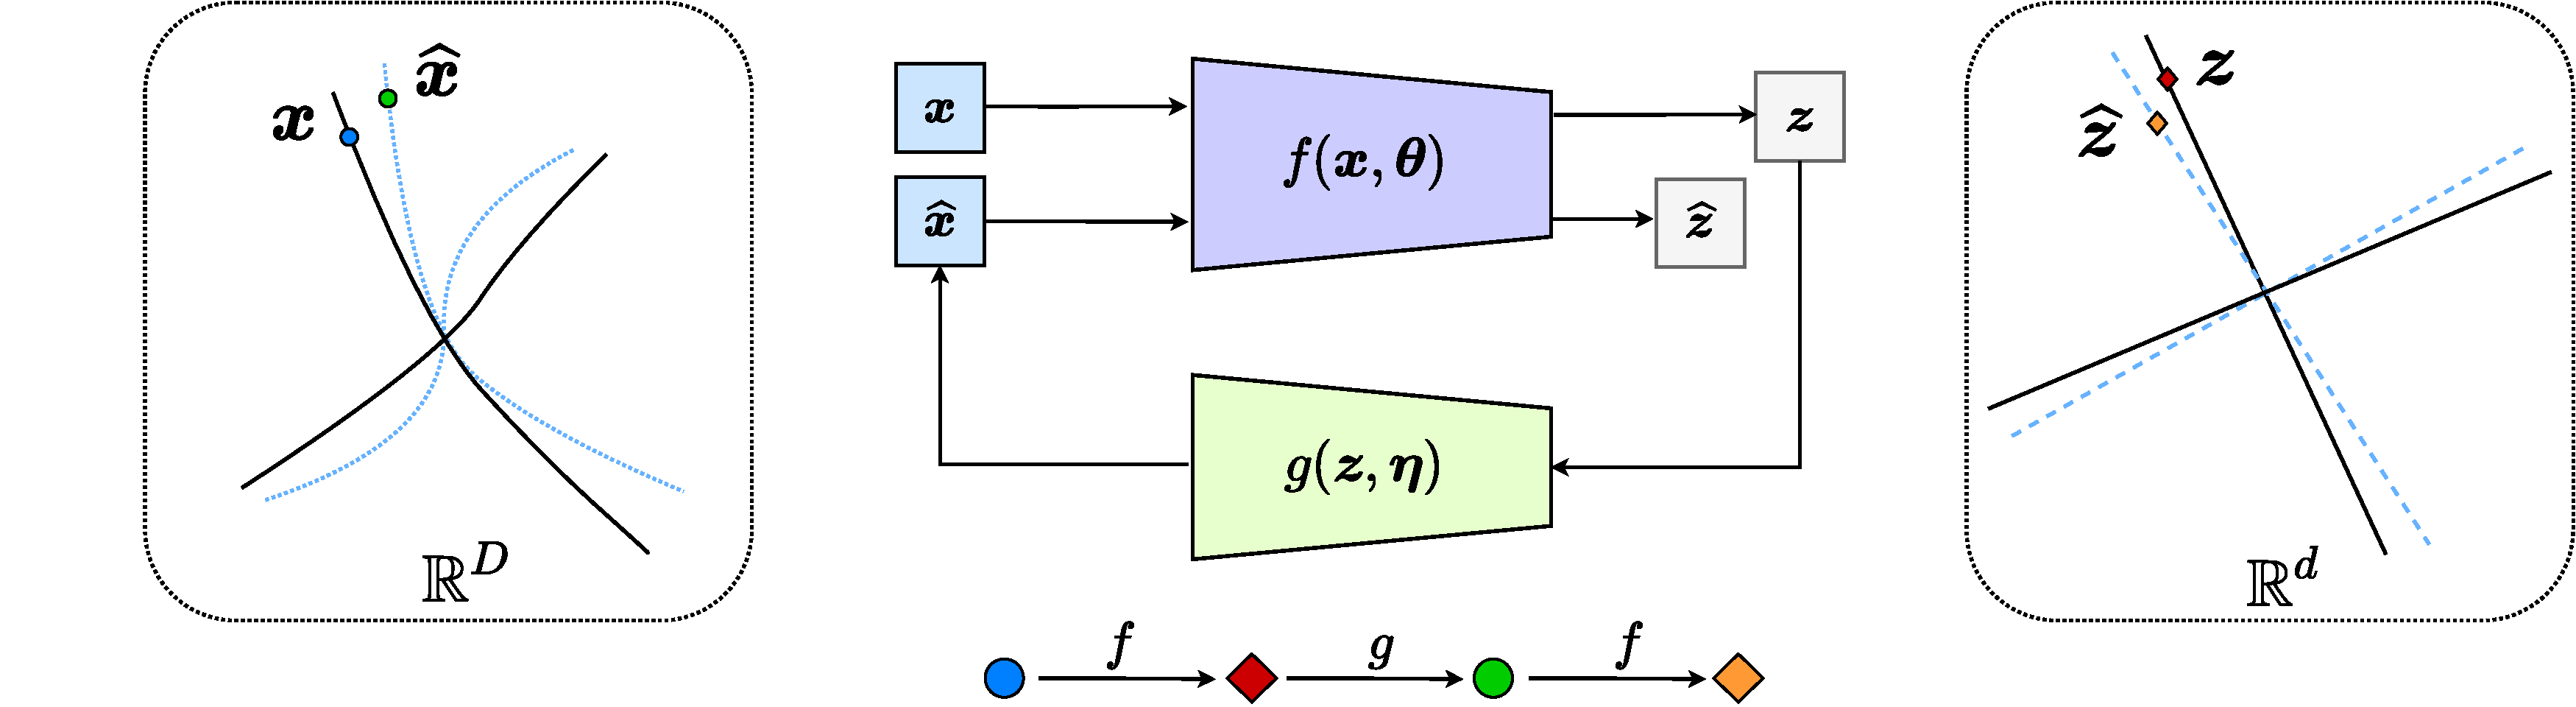
\includegraphics[width=1.0\linewidth]{\toplevelprefix/chapters/chapter5/figs/diagrams_redu_gan_2.pdf}}
\caption{{\bf %
 O Transcriere în Buclă Închisă.} Codificatorul $f$ are roluri duale: învață o reprezentare $\z$ pentru datele $\x$ prin maximizarea reducerii ratei lui $\z$ și este, de asemenea, un „senzor de feedback" pentru orice discrepanță între datele $\x$ și cele decodate $\hat \x$. Decodificatorul $g$ are, de asemenea, roluri duale: este un „controler" care corectează discrepanța dintre $\x$ și $\hat \x$ și, de asemenea, urmărește să minimizeze rata generală de codare pentru reprezentarea învățată.} \label{fig:auto-encoding-closed}
\end{figure}


\paragraph{Codificator și decodificator ca joc cu doi jucători.}
Evident, pentru a asigura că autocodarea învățată este auto-consistentă, obiectivul principal al decodificatorului $g(\cdot, \bm \eta)$ este să {\em minimizeze} distanța dintre $\Z$ și $\hat \Z$. Adică, pentru a învăța $g$, vrem să minimizăm distanța $d(\Z, \hat \Z)$:
\begin{equation}
\min_g d(\Z, \hat \Z) \doteq \min_\eta  \sum_{k=1}^K \Delta R\big(\Z_k, \hat{\Z}_k\big) =  \min_{\bm \eta}  \sum_{k=1}^K \Delta R\big(\Z_k, f(g(\Z_k, \bm \eta),\bm \theta)\big),
\label{eqn:min-distance}
\end{equation}
unde $\Z_k = f(\X_k,\bm \theta)$ și $\hat \Z_k = f(\hat{\X}_k,\bm\theta)$.

\begin{example}
Cineva s-ar putea întreba de ce avem nevoie de maparea $f(\cdot, \bm \theta)$ să funcționeze ca discriminator între $\X$ și $\hat \X$ prin maximizarea $\max_{\bm \theta} \Delta R_\epsilon\big(f(\X,\bm \theta), f(\hat \X, \bm \theta)\big)$. \Cref{fig:decoder} oferă o ilustrare simplă: ar putea exista mulți decodificatori $g$ astfel încât $f\circ g$ să fie o mapare identitate (Id). $f\circ g(\z) = \z $ pentru toți $\z$ în subspațiul $S_{\z}$ din spațiul caracteristic. Cu toate acestea, $g\circ f$ nu este neapărat o hartă de autocodare pentru $\x$ în distribuția originală $S_{\x}$ (aici desenată ca subspațiu pentru simplitate). Adică, $g\circ f(S_{\x}) \not\subset S_{\x}$, cu atât mai puțin $g\circ f(S_{\x}) = S_{\x}$ sau $g\circ f(\x) = \x$. Ar trebui să ne așteptăm că, fără un control atent al imaginii lui $g$, acesta ar fi cazul cu probabilitate mare, mai ales când suportul distribuției lui $\x$ este extrem de mic-dimensional în spațiul original de date de dimensiune înaltă.
\end{example}
\begin{figure}
\centering{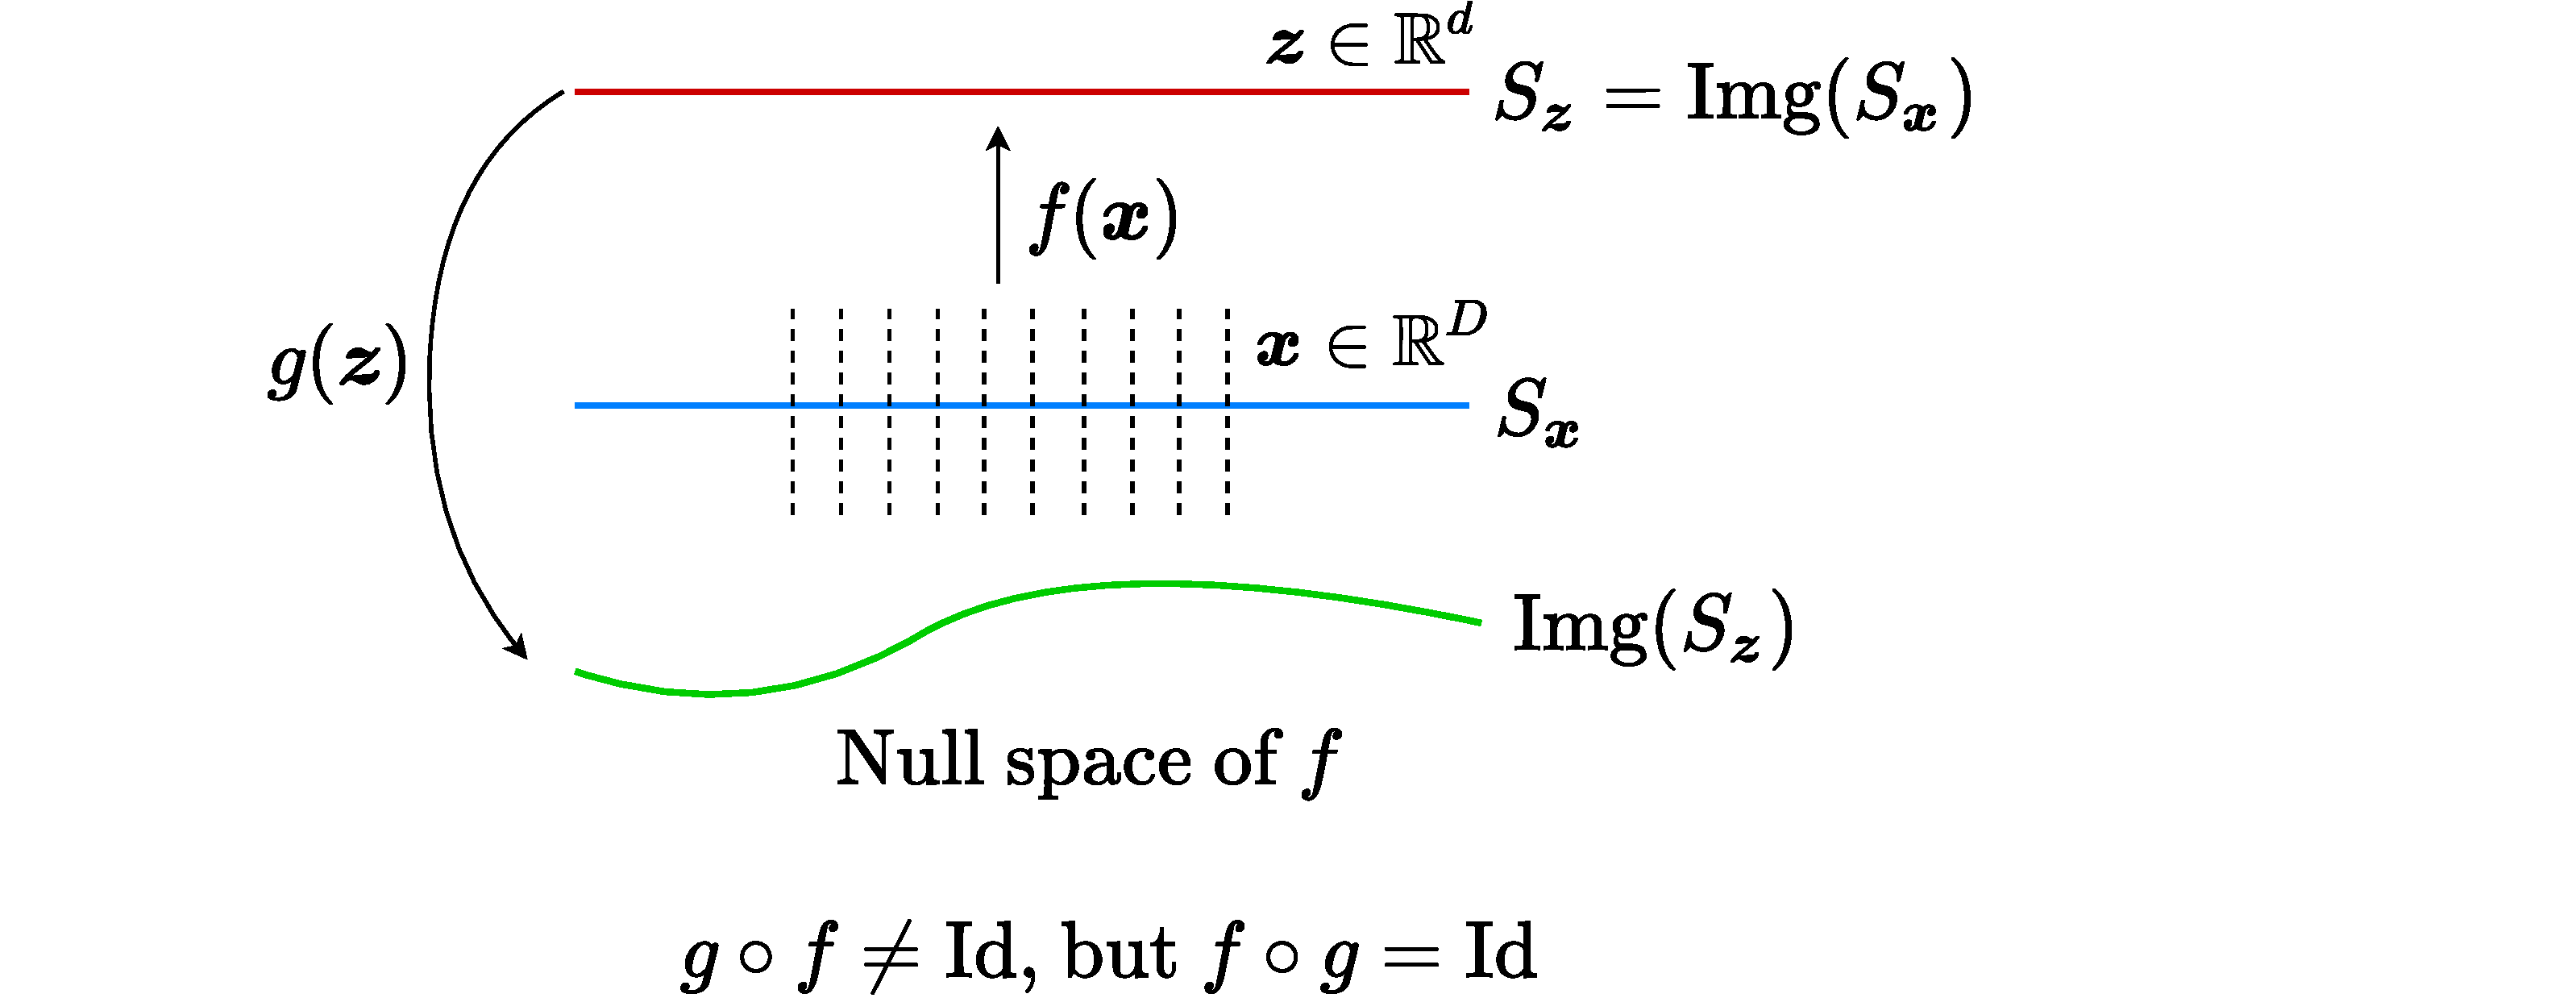
\includegraphics[width=3.0in]{\toplevelprefix/chapters/chapter5/figs/diagrams_fig1.pdf}}
\caption{\textbf{{Încorporări} %
 ale subvarietăților de dimensiune redusă într-un spațiu de dimensiune înaltă.} $S_{\x}$ (albastru) este subvarietatea pentru datele originale $\x$; $S_{\z}$ (roșu) este imaginea lui $S_{\x}$ sub maparea $f$, reprezentând caracteristica învățată $\z$; iar curba verde este imaginea caracteristicii $\z$ sub maparea de decodare $g$.} \label{fig:decoder}
\end{figure}

Comparând natura contractantă și contrastivă a \eqref{eqn:min-distance} și \eqref{eqn:max-distance} asupra aceleiași măsuri de distanță, vedem rolurile codificatorului $f(\cdot, \bm \theta)$ și decodificatorului $g(\cdot, \bm \eta)$ în mod natural ca „{\bf un joc cu doi jucători}": {\em în timp ce codificatorul $f$ încearcă să mărească diferența dintre datele originale și datele lor transcrise, decodificatorul $g$ urmărește să minimizeze diferența.} Acum, pentru comoditate, să definim funcția de „codare în buclă închisă":
\begin{equation}
    h(\x, \bm \theta,\bm \eta) \doteq f\big(g\big(f(\x, \bm \theta), \bm \eta\big), \bm \theta\big): \; \x \mapsto \hat \z.
\end{equation}

În mod ideal, vrem ca această funcție să fie foarte apropiată de $f(\x, \bm \theta)$ sau cel puțin distribuțiile imaginilor lor ar trebui să fie apropiate. Cu această notație, combinând \eqref{eqn:min-distance} și \eqref{eqn:max-distance}, o noțiune în buclă închisă de „distanță" între $\X$ și $\hat \X$ poate fi calculată ca {\em un punct de echilibru} la următorul joc Stackelberg (cf \Cref{sec:minimax}) pentru aceeași utilitate în termenii reducerii ratei:
\begin{equation}
\mathcal{D}(\X, \hat \X) \doteq  \max_{\bm \theta} \min_{\bm \eta} \sum_{k=1}^K \Delta R_\epsilon\big(f(\X_k,\bm \theta), h(\X_k,\bm \theta,\bm \eta)\big).
    \label{eq:MCR2-GAN-pair}
\end{equation}

Observați că aceasta măsoară doar diferența dintre (caracteristicile) datelor originale și versiunea lor transcrisă. Nu măsoară cât de bună este reprezentarea $\Z$ (sau $\hat \Z$) pentru clasele multiple din $\X$ (sau $\hat \X$). În acest scop, putem combina distanța de mai sus cu obiectivele originale de tip MCR$^2$ \eqref{eq:mcr2-formulation}: și anume, reducerea ratei $\Delta R_\epsilon(\Z)$ și $\Delta R_\epsilon(\hat \Z)$ pentru LDR învățat $\Z$ pentru $\X$ și $\hat \Z$ pentru $\hat \X$ decodat. Observați că, deși codificatorul $f$ încearcă să {\em maximizeze} reducerea ratei multi-clasă a caracteristicilor $\Z$ ale datelor $\X$, decodificatorul $g$ ar trebui să {\em minimizeze} reducerea ratei caracteristicilor multi-clasă $\hat \Z$ ale $\hat \X$ decodat. Adică, decodificatorul $g$ încearcă să folosească o rată minimă de codare necesară pentru a obține o calitate bună de decodare.

Prin urmare, jocul Stackelberg general „multi-clasă" pentru învățarea transcrierii în buclă închisă, numit CTRL-Multi, este
\begin{eqnarray}
&&\max_{\bm \theta} \min_{\bm \eta} \mathcal{T}_{\X}(\bm \theta, \bm \eta) \\
&\doteq& \underbrace{\Delta R_\epsilon\big(f(\X,\bm \theta)\big)}_{\text{Codare expansivă}} + \underbrace{\Delta R_\epsilon\big(h(\X,\bm \theta, \bm \eta)\big)}_{\text{Decodare compresivă}} + \sum_{k=1}^K \underbrace{\Delta R_\epsilon\big(f(\X_k,\bm \theta), h(\X_k,\bm \theta,\bm \eta)\big)}_{\text{Codare contrastivă \& Decodare contractivă}}   \\
&=& \Delta R_\epsilon\big(\Z(\bm \theta) \big) + \Delta R_\epsilon\big(\hat \Z(\bm \theta, \bm \eta)\big) + \sum_{k=1}^K \Delta R_\epsilon\big(\Z_k(
\bm \theta), \hat \Z_k(\bm \theta, \bm \eta) \big),
    \label{eq:MCR2-GAN-objective}
\end{eqnarray}
supus anumitor constrângeri (limite superioare sau inferioare) asupra primului termen și celui de-al doilea termen.



Observați că, fără termenii asociați cu partea generativă $h$ sau cu toți acești termeni fixați ca constantă, obiectivul de mai sus este exact obiectivul MCR$^2$ original introdus în \Cref{ch:compression}. Într-un cadru nesupravegheat, dacă vedem fiecare eșantion (și augmentările sale) ca propria sa clasă, formularea de mai sus rămâne exact aceeași. Numărul de clase $k$ este pur și simplu numărul de eșantioane independente. În plus, observați că funcția obiectiv a jocului de mai sus depinde doar de (caracteristicile) datelor $\X$, prin urmare se pot învăța codificatorul și decodificatorul (parametrii) fără necesitatea eșantionării sau potrivirii vreunei distribuții suplimentare (așa cum este de obicei necesar în GAN-uri sau VAE-uri).

Ca un caz special, dacă $\X$ are doar o clasă, jocul Stackelberg se reduce la o formă specială „cu două clase" sau „binară",\footnote{Deoarece primii doi termeni de reducere a ratei devin automat zero} numită CTRL-Binary,
\begin{equation}
 \max_{\bm \theta} \min_{\bm \eta} \mathcal{T}^b_{\X}(\bm \theta, \bm \eta) \doteq \Delta R_\epsilon\big(f(\X,\bm \theta), h(\X,\bm \theta,\bm \eta)\big) = \Delta R_\epsilon\big(\Z(\bm \theta), \hat \Z(\bm \theta, \bm \eta)\big),
    \label{eq:MCR2-GAN-objective-binary}
\end{equation}
între $\X$ și $\hat\X$ decodat prin vizualizarea $\X$ și $\hat \X$ ca două clase $\{\bm 0, \bm 1\}$. Observați că acest caz binar seamănă cu formularea GAN original \eqref{eqn:GAN}. În loc să folosească entropia încrucișată, formularea noastră adoptă o măsură de reducere a ratei mai rafinată, care s-a dovedit a promova diversitatea în reprezentarea învățată în \Cref{ch:compression}.

Uneori, chiar și când $\X$ conține mai multe clase/moduri, se poate vedea totuși toate clasele împreună ca o singură clasă. Apoi, obiectivul binar de mai sus este de a alinia distribuția unită a tuturor claselor cu $\hat \X$ decodat. Aceasta este de obicei o sarcină mai simplă de realizat decât cea multi-clasă \eqref{eq:MCR2-GAN-objective}, deoarece nu necesită învățarea unui CTRL multi-clasă mai rafinat pentru date, așa cum vom vedea mai târziu în experimente. Observați că o caracteristică bună a formulării de mai sus este că {\em toate cantitățile din obiective sunt măsurate în termenii reducerii ratei pentru caracteristicile învățate} (presupunând că caracteristicile devin în cele din urmă gaussiene de subspațiu).

Se poate observa că cadrul de învățare de mai sus se inspiră din corecția erorilor în buclă închisă practicată pe scară largă în sistemele de control cu feedback. Mecanismul în buclă închisă este folosit pentru a forma un sistem general de feedback între cele două rețele de codare și decodare pentru corectarea oricărei „erori" în distribuțiile dintre datele $\x$ și cele decodate $\hat \x$. Folosind terminologia din teoria controlului, se poate vedea rețeaua de codare $f$ ca un „senzor" pentru feedback-ul erorilor, în timp ce rețeaua de decodare $g$ ca un „controler" pentru corecția erorilor. Cu toate acestea, observați că aici „ținta" pentru control nu este un scalar sau un vector de dimensiune finită, ci o distribuție continuă---pentru ca distribuția lui $\hat \x$ să se potrivească cu cea a datelor $\x$. Aceasta este în general o problemă de control într-un spațiu de dimensiune infinită. Spațiul difeomorfismelor posibile ale subvarietăților pe care $f$ încearcă să le modeleze este de dimensiune infinită \cite{Lee2002IntroductionTS}. În mod ideal, sperăm că atunci când senzorul $f$ și controlerul $g$ sunt optimi, distribuția lui $\x$ devine un „punct fix" pentru bucla închisă în timp ce distribuția lui $\z$ atinge o reprezentare liniară discriminativă compactă. Prin urmare, programele minimax \eqref{eq:MCR2-GAN-objective} și \eqref{eq:MCR2-GAN-objective-binary} pot fi interpretate și ca jocuri între un senzor de feedback al erorilor și un controler de reducere a erorilor.

Întrebarea rămasă este dacă cadrul de mai sus poate învăța într-adevăr o reprezentare bună (de autocodare) a unui set de date dat? Înainte de a oferi o justificare teoretică formală (în subsecțiunea următoare), prezentăm câteva rezultate empirice.

\paragraph{Vizualizarea corelației caracteristicilor $\Z$ și caracteristicilor decodate $\hat \Z$.} Vizualizăm similaritatea cosinus între $\Z$ și $\hat{\Z}$ învățate din obiectivul multi-clasă \eqref{eq:MCR2-GAN-objective} pe MNIST, CIFAR-10 și ImageNet (10 clase), care indică cât de aproape este $\hat{\z} = f\circ g(\z)$ de $\z$. Rezultatele din \Cref{fig:justifyz=z} arată că $\Z$ și $\hat{\Z}$ sunt aliniate foarte bine în cadrul fiecărei clase. Modelele bloc-diagonale pentru MNIST sunt mai clare decât cele pentru CIFAR-10 și ImageNet, deoarece imaginile din CIFAR-10 și ImageNet au aspecte vizuale mai diverse.

\begin{figure}[t]
    \begin{subfigure}[t]{0.3\textwidth}
        \centering
        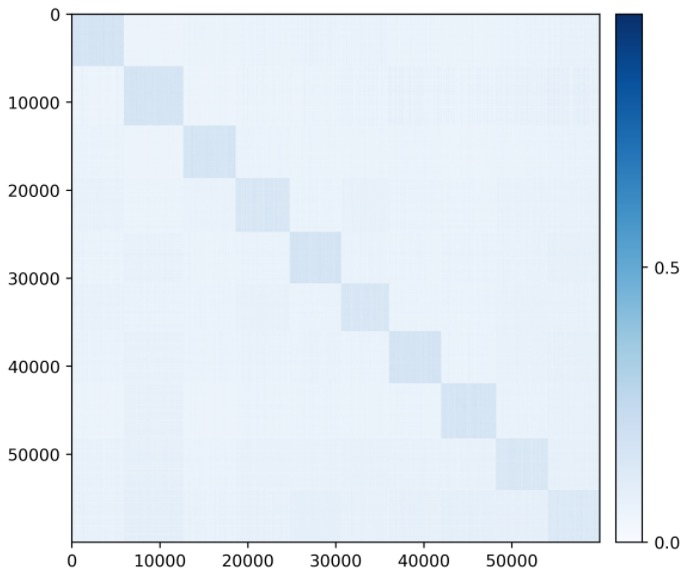
\includegraphics[width=\textwidth]{\toplevelprefix/chapters/chapter5/figs/MNIST_MNIST_ZZhat_heatmap_epo200.png}
        \caption{MNIST}
    \end{subfigure}
    \hfill
    \begin{subfigure}[t]{0.3\textwidth}
        \centering
        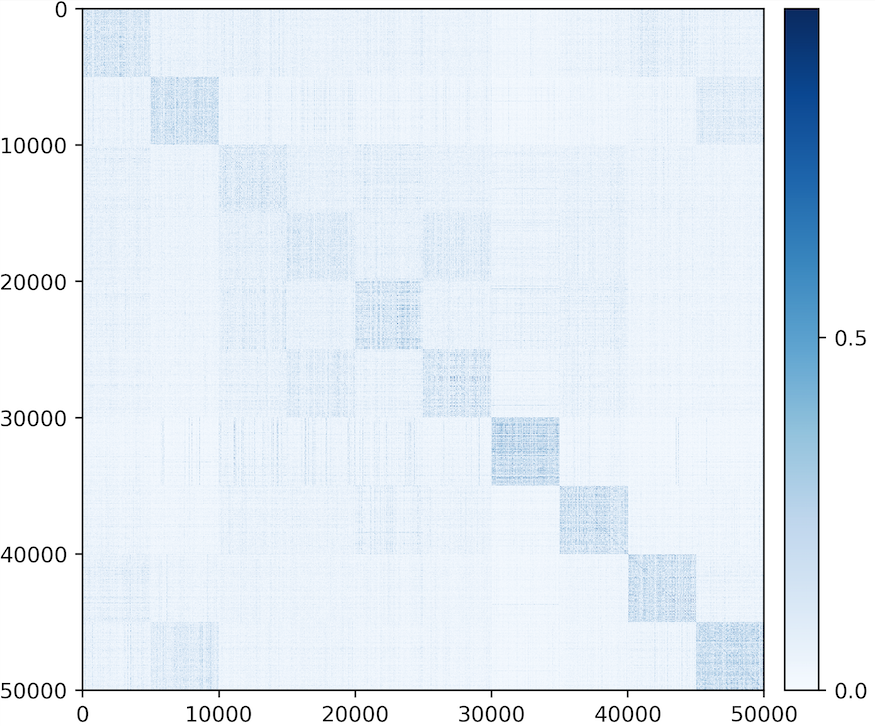
\includegraphics[width=\textwidth]{\toplevelprefix/chapters/chapter5/figs/cifar_heatmat_cifar.png}
        \caption{CIFAR-10}
    \end{subfigure}
    \hfill
    \begin{subfigure}[t]{0.3\textwidth}
        \centering
        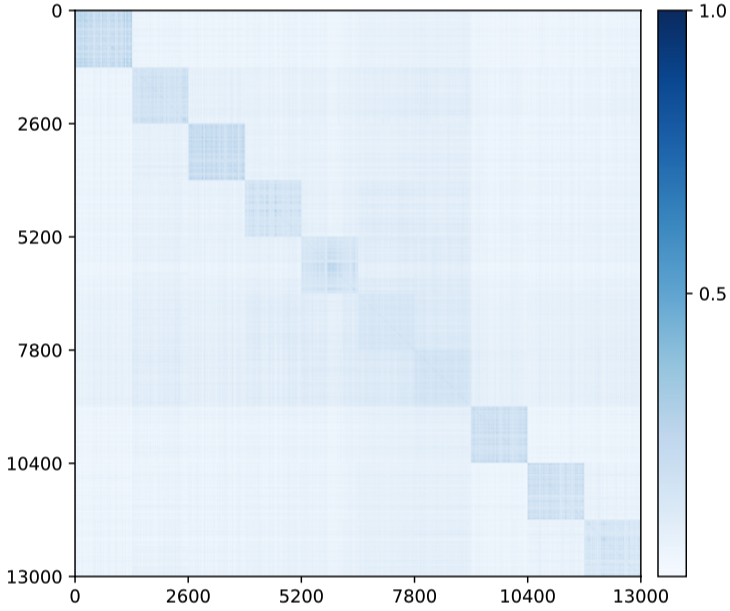
\includegraphics[width=\textwidth]{\toplevelprefix/chapters/chapter5/figs/Imagenet_heatmat_epoch200000.png}
        \caption{ImageNet}
    \end{subfigure}
    \caption{{Vizualizarea} %
    alinierii dintre $\Z$ și $\hat{\Z}$: $|\Z^\top \hat{\Z}|$ în spațiul caracteristic pentru (\textbf{a}) MNIST, (\textbf{b}) CIFAR-10, și~(\textbf{c}) ImageNet-10-Clase.}
    \label{fig:justifyz=z}
\end{figure}




\paragraph{Vizualizarea autocodării datelor $\X$ și celor decodate $\hat \X$.} Comparăm câteva $\X$ reprezentative și $\hat{\X}$ corespunzătoare pe MNIST, CIFAR-10 și ImageNet (10 clase) pentru a verifica cât de aproape este $\hat \x = g\circ f(\x)$ de $\x$. Rezultatele sunt prezentate în \Cref{fig:justify_xhat_equals_x}, iar vizualizările sunt create din eșantioane de antrenament. Vizual, $\hat \x$ autocodat captează fidel caracteristicile vizuale majore din eșantionul de antrenament respectiv $\x$, în special poziția, forma și aspectul. Pentru un set de date mai simplu precum MNIST, imaginile autocodate sunt aproape identice cu originalul.


\begin{figure}[t]
    \begin{subfigure}[t]{0.3\textwidth}
        \centering
        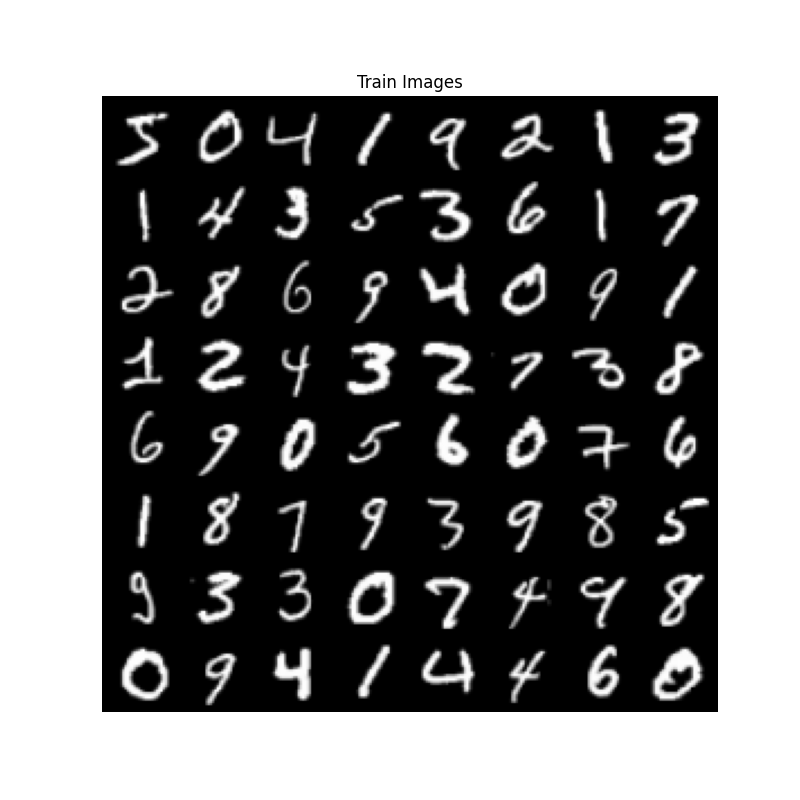
\includegraphics[width=\textwidth]{\toplevelprefix/chapters/chapter5/figs/MNIST_MNIST_train_images_epoch200.png}
        \caption{{\small MNIST $\X$}}
    \end{subfigure}
    \hfill
    \begin{subfigure}[t]{0.3\textwidth}
        \centering
        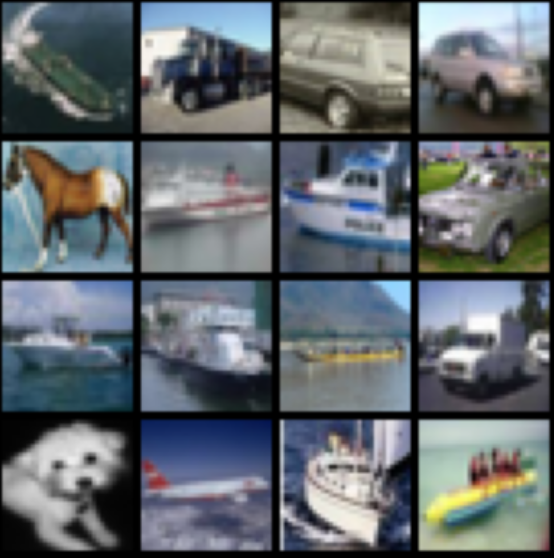
\includegraphics[width=\textwidth]{\toplevelprefix/chapters/chapter5/figs/cifar_input.png}
        \caption{{\small CIFAR-10 $\X$}}
    \end{subfigure}
    \hfill
    \begin{subfigure}[t]{0.3\textwidth}
        \centering
        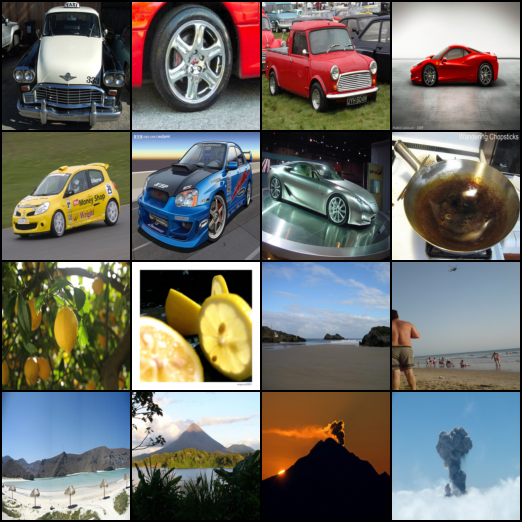
\includegraphics[width=\textwidth]{\toplevelprefix/chapters/chapter5/figs/Imagenet_input.png}
        \caption{{\small ImageNet $\X$}}
    \end{subfigure}

    \begin{subfigure}[t]{0.3\textwidth}
        \centering
        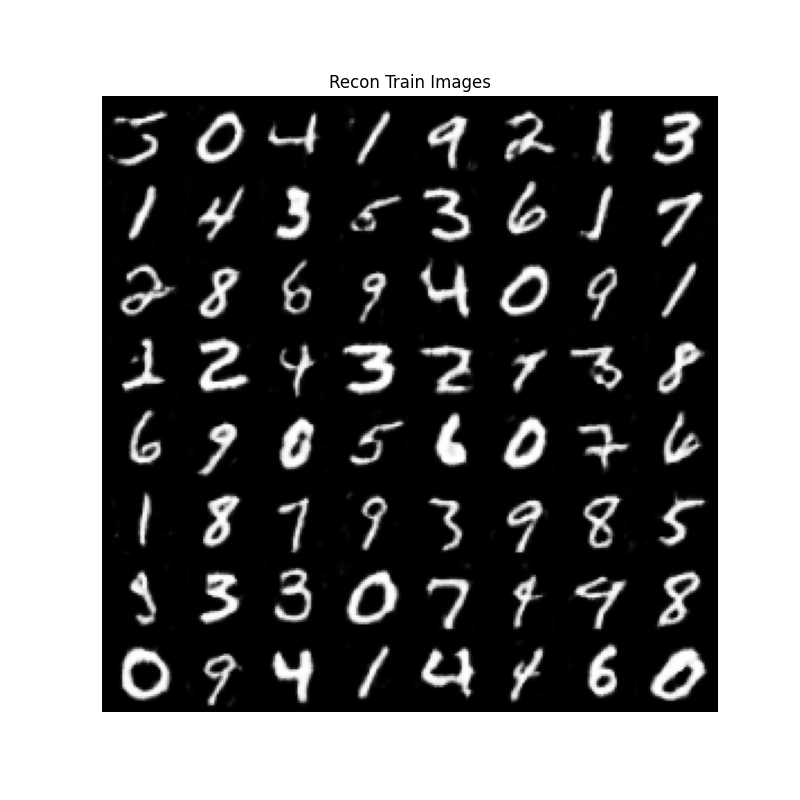
\includegraphics[width=\textwidth]{\toplevelprefix/chapters/chapter5/figs/MNIST_MNIST_train_recon_images_epoch200_multi.png}
        \caption{{\small MNIST $\hat{\X}$}}
    \end{subfigure}
    \hfill
    \begin{subfigure}[t]{0.3\textwidth}
        \centering
        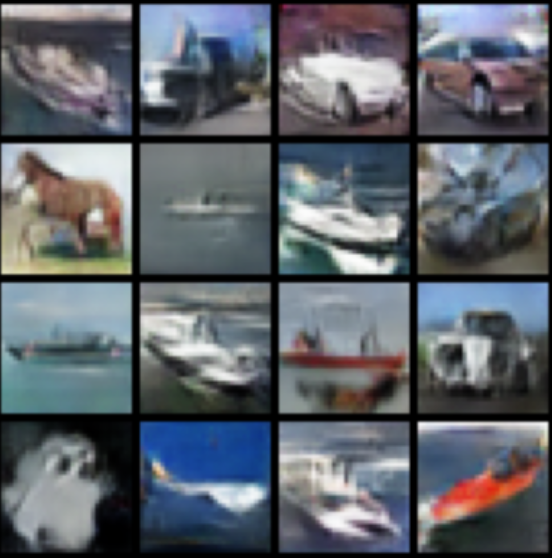
\includegraphics[width=\textwidth]{\toplevelprefix/chapters/chapter5/figs/cifar_reconstruct.png}
        \caption{{\small CIFAR-10 $\hat{\X}$}}
    \end{subfigure}
    \hfill
    \begin{subfigure}[t]{0.3\textwidth}
        \centering
        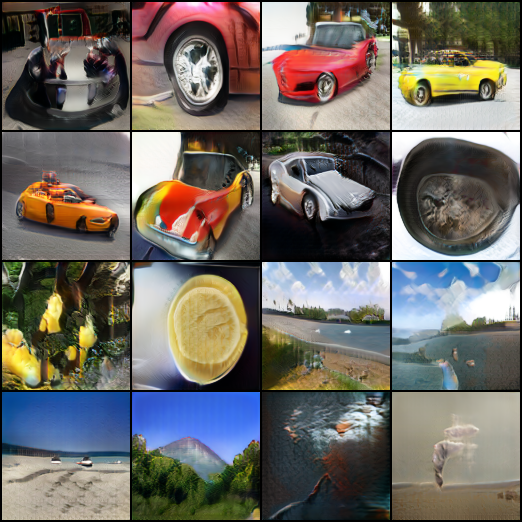
\includegraphics[width=\textwidth]{\toplevelprefix/chapters/chapter5/figs/Imagenet_reconstruct.png}
        \caption{{\small ImageNet $\hat{\X}$}}
    \end{subfigure}
    \caption{Vizualizarea proprietății de auto-codare a transcrierii învățate în buclă închisă \mbox{($\x \approx \hat{\x} = g\circ f(\x)$)} pe MNIST, CIFAR-10 și ImageNet (măriți pentru o vizualizare mai bună).}
    \label{fig:justify_xhat_equals_x}
\end{figure}


\subsection{Un Amestec de Gaussiene de Dimensiune Redusă}

În cele de mai sus, am argumentat că este posibil să formulăm problema învățării unei distribuții de date ca o problemă de autocodare în buclă închisă. Am văzut, de asemenea, empiric că o astfel de schemă pare să funcționeze. Întrebarea rămasă este când și de ce ar trebui să funcționeze o astfel de schemă. Este dificil să răspundem la această întrebare pentru cazurile cele mai generale cu distribuții arbitrare de date. Cu toate acestea, ca de obicei, să vedem dacă putem ajunge la o justificare riguroasă pentru cazul ideal când distribuția datelor este un amestec de subspații de dimensiune redusă sau gaussiene de rang redus. O caracterizare și înțelegere clară a acestui caz special important ar arunca lumină asupra cazurilor mai generale.\footnote{Deoarece majoritatea distribuțiilor cu structuri de dimensiune redusă pot fi bine aproximate de această familie de distribuții.}

În acest scop, să presupunem mai întâi că \(\vX\) este distribuit conform unui amestec de gaussiene de dimensiune redusă, iar eticheta (adică atribuirea subspațiului) pentru \(\vX\) este dată de \(\vy\). Apoi, să stabilim o problemă de optimizare minimax pentru a învăța distribuția datelor, să zicem prin învățarea unei codări a \(\vX\) în reprezentări \(\vZ\) care sunt suportate pe un amestec de subspații \textit{ortogonale}, și o decodare a \(\vZ\) înapoi în \(\vX\). Apoi, reprezentarea pe care vrem să o obținem este maximizată de versiunea discutată anterior a câștigului de informație, adică \( \Delta R_{\epsilon}(\vZ) = R_{\epsilon}(\vZ) - \sum_{k=1}^K R_{\epsilon}(\bm Z_k) \), care impune ca reprezentarea \(\vZ_{k}\) a fiecărei clase \(k\) să acopere un subspațiu care este ortogonal pe subspațiile suport ale altor clase. Modul de a măsura consistența decodării este, ca înainte, dat de \(\sum_{k = 1}^{K}\Delta R_\epsilon(\vZ_{k}, \hat{\vZ}_{k})\), care impune ca reprezentarea \(\vZ_{k}\) și autocodarea sa \(\hat{\vZ}_{k}\) pentru fiecare clasă \(k\) să acopere același subspațiu. Astfel, putem stabili un joc Stackelberg simplificat:
\begin{equation}\label{eq:ctrl_msp_game}
    \max_{\bm \theta}\min_{\bm \eta}\bc{\Delta R_\epsilon(\vZ(\bm \theta)) + \sum_{k = 1}^{K}\Delta R_\epsilon(\vZ_{k}(\bm \theta), \hat{\vZ}_{k}(\bm \theta, \bm \eta))}
\end{equation}
Observați că aceasta este o configurare mai simplă decât ceea ce este folosit în practică---nu există un termen \(\Delta R_\epsilon(\hat{\vZ})\), de exemplu, și lucrăm în cadrul supravegheat cu etichete de clasă (deși tehnicile folosite pentru a demonstra următorul rezultat sunt ușor de extins la formulări nesupravegheate). De asemenea, consistența reprezentărilor este măsurată doar într-un sens distributional prin \(\Delta R_\epsilon\) (deși aceasta poate fi înlocuită cu o metrică de distanță pe eșantioane, cum ar fi norma \(\ell_{2}\) dacă se dorește, și se pot trage concluzii echivalente, \textit{mutatis mutandis}).

În condiții blânde, pentru a realiza codificatorul și decodificatorul doriți care realizează \(\vZ\) dintr-o sursă de date \(\vX\) care este deja distribuită conform unui amestec de gaussiene corelate de dimensiune redusă, avem nevoie doar de un codificator și decodificator liniar pentru a desface și albi gaussienele. Studiem apoi acest cadru în cazul în care \(\bm \theta\) și \(\bm \eta\) parametrizează matrici a căror normă de operator este constrânsă.

Vrem să înțelegem ce tipuri de optimi sunt învățate în acest cadru. Un concept de soluție potrivit pentru acest tip de joc, unde soluția optimă a decodificatorului este definită doar în raport cu codificatorul (și nu, în special, în raport cu o altă proprietate intrinsecă a decodificatorului), este un \textit{echilibru Stackelberg} unde decodificatorul urmează codificatorul.
Și anume, la un astfel de echilibru, decodificatorul ar trebui să-și optimizeze obiectivul; între timp, codificatorul ar trebui să-și optimizeze obiectivul, având în vedere că, indiferent de ce alege, decodificatorul va alege un răspuns optim (care poate afecta obiectivul codificatorului). În termeni de teorie a jocurilor, este ca și cum decodificatorul merge \textit{al doilea}: își alege ponderile după codificator, iar atât codificatorul cât și decodificatorul încearcă să-și optimizeze obiectivul în lumina acestui fapt. Este tractabil computațional să învățăm echilibrele secvențiale prin metode de gradient prin \textit{optimizare alternativă}, unde fiecare parte folosește rate de învățare diferite. Expunerea detaliată a echilibrelor secvențiale depășește scopul acestei cărți și oferim mai multe detalii tehnice în \Cref{sec:minimax}. În acest cadru, avem următorul rezultat:
\begin{theorem}[\cite{pai2022pursuit}, Prescurtat]\label{thm:ctrl_theory}
    Să presupunem că \(\vX\) este distribuit pe un amestec de subspații. În anumite condiții realiste, dar tehnice, este valabil că toate echilibrele secvențiale ale \eqref{eq:ctrl_msp_game} respectă:
    \begin{itemize}
        \item \(\vZ_{k}\) se află pe subspații ortogonale și sunt izotrope pe acele subspații, adică maximizează câștigul de informație.
        \item Autocodarea este auto-consistentă, adică subspațiile acoperite de \(\vZ_{k}\) și \(\hat{\vZ}_{k}\) sunt aceleași pentru toți \(k\).
    \end{itemize}
\end{theorem}
Această noțiune de auto-consistență este maximul pe care îl putem aștepta dacă există doar ipoteze geometrice asupra datelor, adică nu există ipoteze statistice. Dacă presupunem că coloanele lui \(\vX\) sunt extrase dintr-un model de amestec gaussian de rang redus, atunci versiuni analoge ale acestei teoreme certifică că \(\vZ_{k}\) sunt, de asemenea, gaussiene de rang redus a căror covarianță este izotropă, de exemplu.
În esență, acest rezultat validează, prin cazul simplu al amestecurilor gaussiene pe subspații, că jocurile minimax pentru optimizarea câștigului de informație și auto-consistenței pot obține soluții optime.






\section{Învățarea Continuă a Reprezentărilor Auto-Consistente}
\label{sec:continuous}

\subsection{Învățare Incrementală pe Clase}
\label{sec:class-wise-incremental}

După cum am văzut, rețelele neuronale profunde au demonstrat o mare capacitate de a învăța reprezentări pentru sute sau chiar mii de clase de obiecte, atât în contexte discriminative cât și generative. Cu toate acestea, rețelele trebuie de obicei antrenate offline, cu date eșantionate uniform din toate clasele simultan. Este cunoscut faptul că atunci când o rețea (în buclă deschisă) este actualizată pentru a învăța clase noi fără date din cele vechi, cunoștințele învățate anterior vor cădea victimă problemei {\em uitării catastrofale} \cite{McCloskey1989catastrophic}. Aceasta este cunoscută în neuroștiință ca dilema stabilitate-plasticitate: provocarea de a asigura că un sistem neuronal poate învăța dintr-un mediu nou, păstrând în același timp cunoștințele esențiale din cele anterioare \cite{Grossberg1987CompetitiveLF}.

În contrast, sistemele neuronale naturale (de exemplu, creierul animalelor) nu par să sufere deloc de o astfel de uitare catastrofală. Ele sunt capabile să dezvolte memorie nouă a obiectelor noi, păstrând în același timp memoria obiectelor învățate anterior. Această abilitate, pentru sistemele neuronale naturale sau artificiale, este adesea denumită {\em învățare incrementală, învățare continuă, învățare secvențială} sau {\em învățare pe viață} \cite{controlled-forgetting}.



Deși multe lucrări recente au evidențiat modul în care sistemele neuronale artificiale pot fi antrenate în moduri mai flexibile, cele mai puternice eforturi existente pentru a răspunde dilemei stabilitate-plasticitate pentru rețelele neuronale artificiale necesită de obicei fie stocarea exemplarelor brute \cite{icarl,chaudhry2019tiny}, fie furnizarea de mecanisme externe \cite{EWC}. Exemplarele brute, în special în cazul intrărilor de dimensiune înaltă precum imaginile, sunt costisitoare și dificil de scalat, în timp ce mecanismele externe---care includ de obicei rețele secundare și spații de reprezentare pentru redare generativă, alocarea incrementală a resurselor de rețea, duplicarea rețelei sau izolarea explicită a părților folosite și nefolosite ale rețelei---necesită euristici și implică costuri ascunse.


Aici suntem interesați de un cadru de învățare incrementală care este similar cu natura. Aceasta contracarează aceste practici existente cu două calități cheie.
\begin{enumerate}
    \item Prima este că ar trebui să fie \emph{bazată pe memorie.} Când învățăm clase noi, nu sunt disponibile exemplare brute ale claselor vechi pentru a antrena rețeaua împreună cu date noi. Aceasta implică că trebuie să ne bazăm pe o „memorie" compactă și astfel structurată învățată pentru clasele vechi, cum ar fi reprezentările generative învățate incremental ale claselor vechi, precum și mapările asociate de codare și decodare \cite{fearnet}.
    \item A doua este că ar trebui să fie \emph{autonomă}. Învățarea incrementală are loc într-un singur sistem neuronal cu o capacitate fixă și într-un spațiu comun de reprezentare. Capacitatea de a minimiza uitarea este implicată de optimizarea unui obiectiv general de învățare, fără rețele externe, modificări arhitecturale sau mecanisme de alocare a resurselor.
\end{enumerate}

Structurile liniare incoerente pentru caracteristicile diferitelor clase seamănă foarte mult cu modul în care obiectele sunt codificate în diferite zone ale cortexului inferotemporal al creierului animalelor \cite{Chang-Cell-2017,Bao2020AMO}. Transcrierea în buclă închisă $\X \rightarrow \Z \rightarrow \hat{\X} \rightarrow \hat{\Z}$ seamănă, de asemenea, cu mecanismele ipotezate popular pentru formarea memoriei \cite{2020Vandeven,Josselyn2020MemoryER}. Aceasta conduce la o întrebare: deoarece memoria în creier este formată într-un mod incremental, poate cadrul de transcriere în buclă închisă de mai sus să sprijine și învățarea incrementală?

\paragraph{Eșantionare și redare a memoriei LDR.} {\em Structurile} liniare simple ale LDR o fac unic potrivită pentru învățarea incrementală: distribuția caracteristicilor $\Z_j$ ale fiecărei clase învățate anterior poate fi reprezentată explicit și concis printr-un subspațiu principal $\mathcal{S}_j$ în spațiul caracteristic. Pentru a păstra memoria unei clase vechi $j$, trebuie doar să păstrăm subspațiul în timp ce învățăm clase noi. În acest scop, eșantionăm pur și simplu $m$ caracteristici prototip reprezentative pe subspațiu de-a lungul celor mai mari $r$ componente principale și denotăm aceste caracteristici ca $\Z_{j,old}$. Datorită structurilor liniare simple ale LDR, putem eșantiona din $\Z_{j,old}$ calculând media și covarianța lui $\Z_{j,old}$ după învățarea clasei $j$. Stocarea necesară este extrem de mică, deoarece trebuie să stocăm doar medii și covarianțe, care sunt eșantionate după necesitate. Să presupunem că un total de $t$ clase vechi au fost învățate până acum. Dacă caracteristicile prototip, notate $\Z_{old} \doteq [\Z^1_{old},\ldots, \Z^t_{old}]$, pentru toate aceste clase pot fi păstrate când învățăm clase noi, subspațiile $\{\mathcal{S}_j\}_{j=1}^t$ reprezentând memoria trecută vor fi păstrate de asemenea. Detalii despre eșantionare și calcularea mediei și covarianței pot fi găsite în lucrarea \cite{tong2023incremental}.

\begin{figure*}[t]
\centering
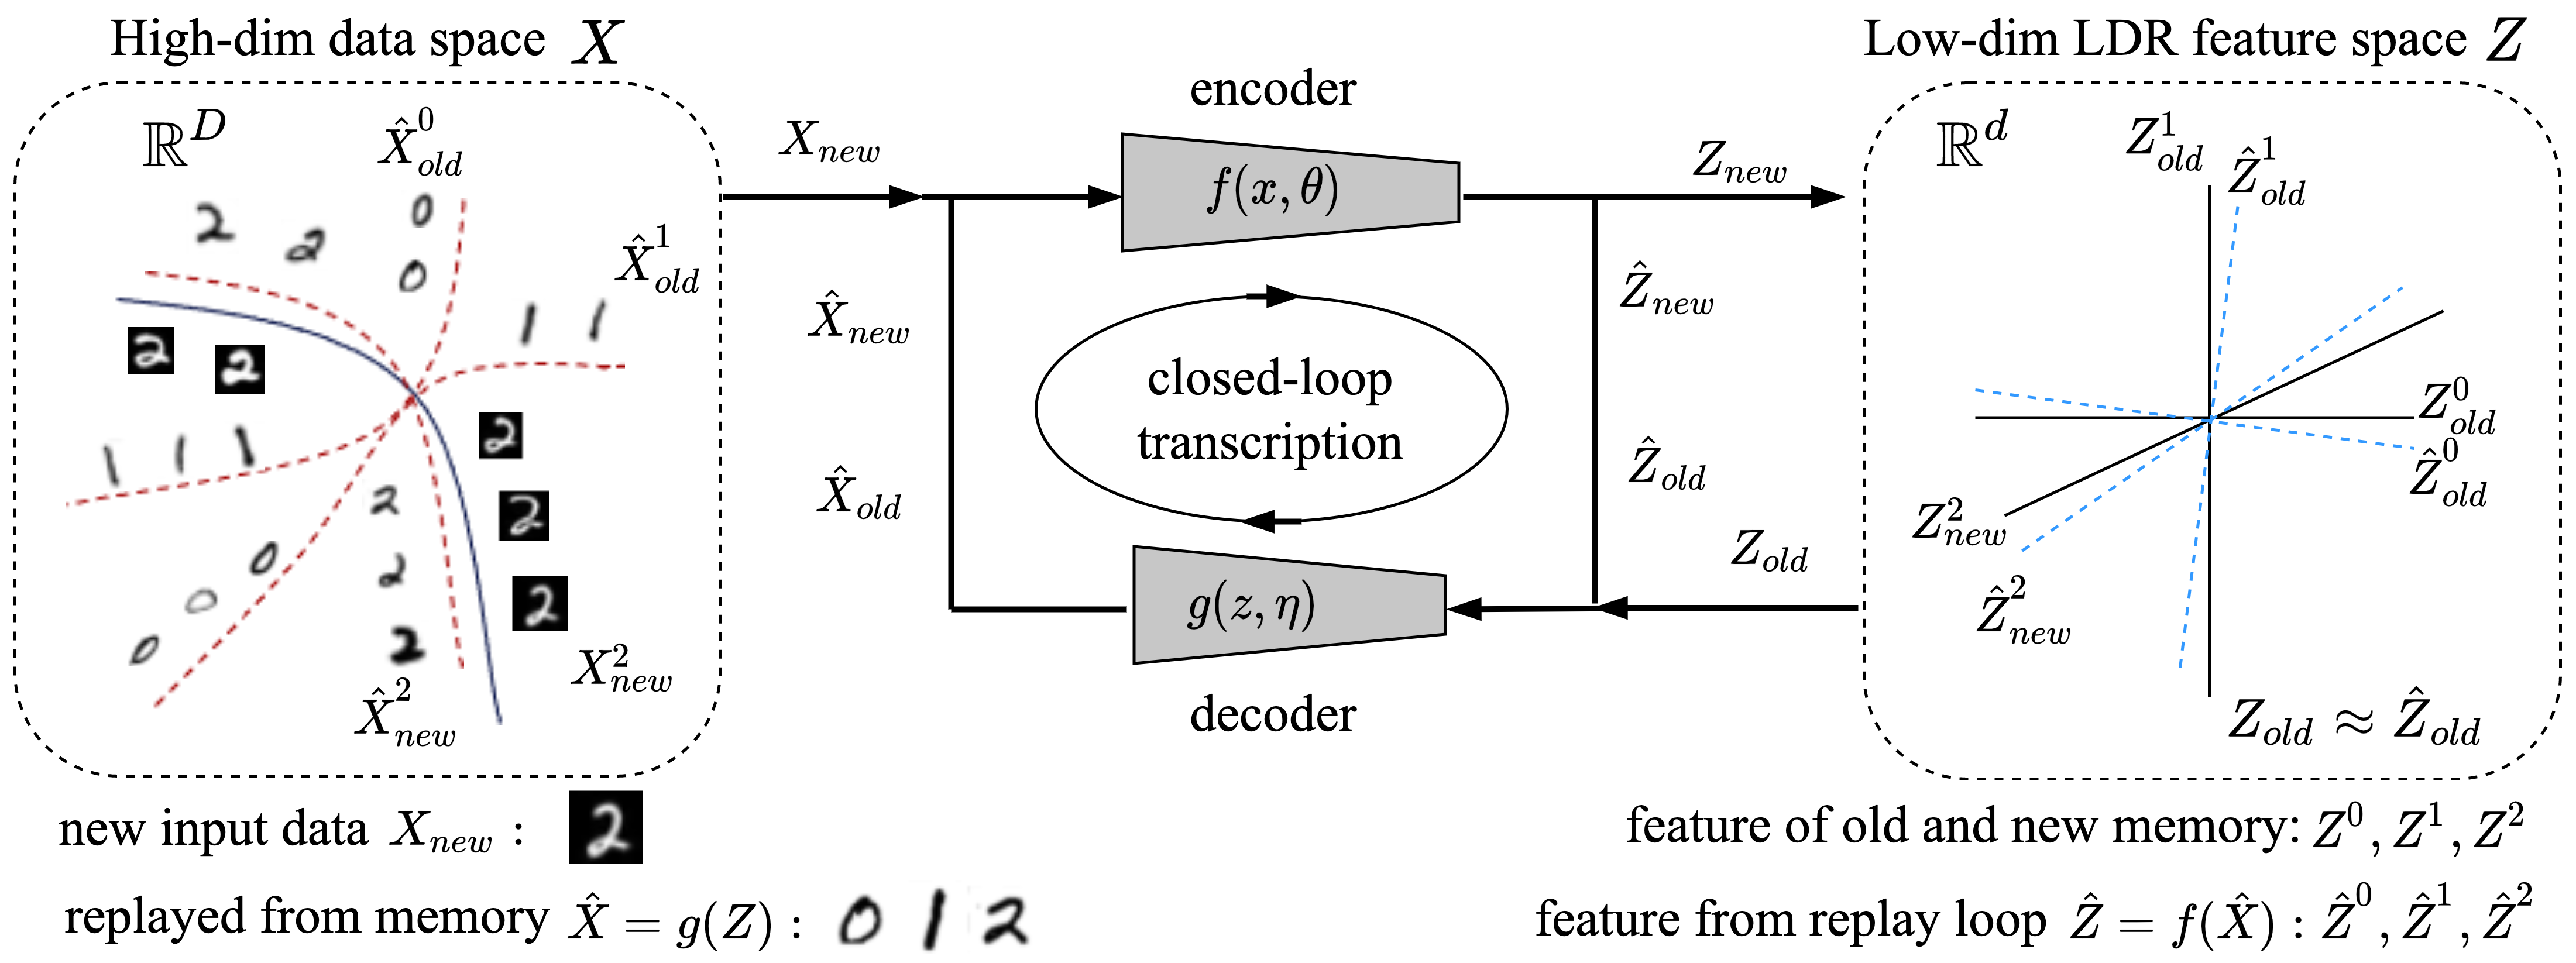
\includegraphics[width=0.9\textwidth]{\toplevelprefix/chapters/chapter5/figs/framework-v7.png}
\caption{\textbf{Cadrul general} al învățării incrementale bazate pe transcriere în buclă închisă pentru o memorie LDR structurată. Este necesară doar o singură rețea de codare-decodare complet autonomă: pentru o nouă clasă de date $\X_{new}$, o nouă memorie LDR $\Z_{new}$ este învățată incremental ca un joc minimax între codificator și decodificator supus constrângerii că memoria veche a claselor trecute $\Z_{old}$ este intactă prin transcrierea în buclă închisă (sau redare): $\Z_{old} \approx \hat{\Z}_{ old} = f(g(\Z_{ old}))$.
\vspace{-0.2in}}
\label{fig:framework}
\end{figure*}

\paragraph{Învățarea incrementală LDR cu o constrângere de memorie veche.}
Observați că, cu autocodarea învățată \eqref{eqn:autoencoding-ch6}, se pot reda și utiliza imaginile, să zicem $\hat\X_{old} = g(\Z_{old}, \bm \eta)$, asociate cu caracteristicile memoriei pentru a evita uitarea în timp ce învățăm clase noi. Aceasta este de obicei modul în care modelele generative au fost folosite pentru metodele anterioare de învățare incrementală. Cu toate acestea, cu cadrul în buclă închisă, redarea explicită a imaginilor din caracteristici nu este necesară. Memoria trecută poate fi păstrată eficient prin optimizare exclusiv pe caracteristicile în sine.

Considerați sarcina de a învăța incremental o nouă clasă de obiecte.\footnote{Desigur, se poate lua în considerare și cadrul mai general în care sarcina conține un lot mic de clase noi, fără modificări serioase.} Denotăm un set de eșantioane nou corespunzător ca $\X_{new}$. Caracteristicile lui $\X_{new}$ sunt notate ca $\Z_{new}(\bm \theta) = f(\X_{new}, \bm \theta)$. Le concatenăm împreună cu caracteristicile prototip ale claselor vechi $\Z_{old}$ și formăm $\Z = [\Z_{new}(\bm \theta), \Z_{old}]$. Denotăm imaginile redate din toate caracteristicile ca $\hat{\X} = [{\hat{\X}_{new}(\bm \theta,\bm \eta)}, {\hat{\X}_{old}(\bm \eta)}]$, deși nu trebuie de fapt să le calculăm sau să le folosim explicit. Avem nevoie doar de caracteristicile imaginilor redate, notate $\hat{\Z} = f(\hat{\X}, \bm \theta) =  [{\hat{\Z}_{new}(\bm \theta,\bm \eta)}, {\hat{\Z}_{old}(\bm \theta,\bm \eta)}]$.


Oglindind motivația pentru obiectivul CTRL multi-clasă \eqref{eq:MCR2-GAN-objective}, am dori ca caracteristicile noii clase $\Z_{new}$ să fie incoerente cu toate cele vechi $\Z_{old}$. Deoarece $\Z_{new}$ este singura clasă nouă ale cărei caracteristici trebuie învățate, obiectivul \eqref{eq:MCR2-GAN-objective} se reduce la cazul în care $k=1$:
\begin{equation}
\min_{\bm \eta} \max_{\bm \theta} \Delta{R_\epsilon(\Z)} + \Delta{R_\epsilon(\hat{\Z})}+\Delta{R_\epsilon(\Z_{new},\hat{\Z}_{new})}.
\label{eqn:unconstrained-minimax}
\end{equation}
Cu toate acestea, când actualizăm parametrii rețelei $(\bm \theta,\bm \eta)$ pentru a optimiza caracteristicile pentru noua clasă, mapările actualizate $f$ și $g$ vor schimba și caracteristicile claselor vechi. Prin urmare, pentru a minimiza distorsiunea reprezentărilor clasei vechi, putem încerca să impunem $\mbox{Cov}(\Z_{j,old}) = \mbox{Cov}(\hat{\Z}_{j,old})$. Cu alte cuvinte, în timp ce învățăm clase noi, impunem ca memoria claselor vechi să rămână „auto-consistentă" prin bucla de transcriere:
\begin{equation}
\Z_{old} \xrightarrow{\hspace{2mm} g(\z,\bm \eta) \hspace{2mm}} \hat \X_{old} \xrightarrow{\hspace{2mm} f(\x, \bm \theta)\hspace{2mm}} \ \hat \Z_{old}.
\end{equation}
Matematic, aceasta este echivalentă cu setarea
$$\Delta R_\epsilon(\Z_{old},\hat{\Z}_{old}) \doteq  \sum_{j=1}^t \Delta R_\epsilon(\Z_{j,old},\hat{\Z}_{j,old}) = 0.$$
Prin urmare, programul minimax de mai sus \eqref{eqn:unconstrained-minimax} este revizuit ca un joc minimax {\em constrâns}, pe care îl numim {\em transcriere incrementală în buclă închisă} (i-CTRL).
Obiectivul acestui joc este identic cu obiectivul CTRL multi-clasă standard \eqref{eq:MCR2-GAN-objective}, dar include doar o constrângere suplimentară:
\begin{eqnarray}
\min_{\bm \eta} \max_{\bm \theta}  &&\Delta{R_\epsilon(\Z)}+\Delta{R_\epsilon(\hat{\Z})}+\Delta{R_\epsilon(\Z_{new},\hat{\Z}_{new})} \nonumber\\
&& \mbox{supus la} \quad  \Delta R(\Z_{old},\hat{\Z}_{old}) = 0.
\label{eqn:constrained-minimax}
\end{eqnarray}

În practică, programul minimax constrâns poate fi rezolvat prin minimizare și maximizare {\em alternativă} între codificatorul $f(\cdot, \bm \theta)$ și decodificatorul $g(\cdot, \bm \eta)$ după cum urmează:
\begin{eqnarray}
&\max_{\bm \theta}  &\Delta{R_\epsilon(\Z)}\!+\!\Delta{R_\epsilon(\hat{\Z})}\!+\!\lambda\cdot  \Delta{R_\epsilon(\Z_{new},\hat{\Z}_{new})} - \gamma\cdot \Delta{R_\epsilon(\Z_{old},\hat{\Z}_{old})}, \label{eqn:relaxed-max}\\
&\min_{\bm \eta} &\Delta{R_\epsilon(\Z)}\!+\!\Delta{R_\epsilon(\hat{\Z})}\!+\!\lambda\cdot \Delta{R_\epsilon(\Z_{new},\hat{\Z}_{new})} + \gamma\cdot \Delta{R_\epsilon(\Z_{old},\hat{\Z}_{old})}; \label{eqn:relaxed-min}
\end{eqnarray}
unde constrângerea $\Delta R_\epsilon(\Z_{old},\hat{\Z}_{old}) = 0$ din \eqref{eqn:constrained-minimax} a fost convertită (și relaxată) într-un termen Lagrangian cu un coeficient corespunzător $\gamma$ și semn. Introducem suplimentar un alt coeficient $\lambda$ pentru ponderarea termenului de reducere a ratei asociat cu datele noi.



\paragraph{Memorie optimă comună prin revizuire incrementală.}
După cum vom vedea, programul minimax constrâns de mai sus poate deja obține performanțe de ultimă generație pentru învățarea incrementală. Cu toate acestea, dezvoltarea unei memorii optime pentru {\em toate clasele} nu se poate baza doar pe uitarea grațioasă. Chiar și pentru oameni, dacă o clasă de obiecte este învățată o singură dată, ar trebui să ne așteptăm ca memoria învățată să se estompeze pe măsură ce continuăm să învățăm altele noi, cu excepția cazului în care memoria poate fi consolidată prin revizuirea claselor vechi de obiecte.

Pentru a emula această fază de formare a memoriei, după învățarea incrementală a unui întreg set de date, putem reveni să revizuim din nou toate clasele, câte o clasă pe rând. Ne referim la parcurgerea tuturor claselor o dată ca un „ciclu" de revizuire.\footnote{pentru a distinge de termenul „epocă" folosit în cadrul convențional de învățare comună.} Dacă este necesar, pot fi efectuate mai multe cicluri de revizuire. Este destul de așteptat ca revizuirea să poată îmbunătăți memoria (LDR) învățată. Dar oarecum surprinzător, cadrul în buclă închisă ne permite să revizuim chiar și într-un mod „{nesupravegheat pe clase}": când revizuim datele unei clase vechi, să zicem $\X_j$, sistemul nu are nevoie de eticheta clasei și poate trata pur și simplu $\X_j$ ca o clasă nouă $\X_{new}$. Adică, sistemul optimizează același program mini-max constrâns \eqref{eqn:constrained-minimax} fără nicio modificare; după ce sistemul este optimizat, se poate identifica subspațiul nou învățat acoperit de $\Z_{new}$ și îl folosește pentru a înlocui sau fuziona cu vechiul subspațiu $\mathcal{S}_j$. După cum arată experimentele noastre, un astfel de proces de revizuire incrementală nesupravegheată pe clase poate îmbunătăți treptat atât performanța discriminativă cât și cea generativă a memoriei LDR, convergând în cele din urmă la cea a unei memorii învățate în comun.

\paragraph{Verificare experimentală.}
Arătăm câteva rezultate experimentale pe următoarele seturi de date: MNIST \cite{lecun1998gradient} și CIFAR-10 \cite{krizhevsky2014cifar}. Toate experimentele sunt efectuate pentru cadrul mai dificil de învățare pe clase. Pentru ambele MNIST și CIFAR-10, cele 10 clase sunt împărțite în 5 sarcini cu 2 clase fiecare sau 10 sarcini cu 1 clasă fiecare. Pentru codificatorul $f$ și decodificatorul $g$, adoptăm o arhitectură de rețea foarte simplă modificată din DCGAN \cite{radford2016unsupervised}, care este doar o rețea convoluțională cu {\em patru straturi}. Aici arătăm doar câteva rezultate vizuale calitative; mai multe experimente și analize analitice pot fi găsite în lucrarea \cite{tong2023incremental}.

\paragraph{Vizualizarea proprietăților de auto-codare.}
Începem prin vizualizarea calitativă a unor imagini reprezentative $\X$ și celor redate corespunzătoare $\hat{\X}$ pe MNIST și CIFAR-10. Modelul este învățat incremental cu seturile de date împărțite în 5 sarcini. Rezultatele sunt prezentate în \Cref{fig:justify_xhat_equals_x_incremental}, unde observăm că $\hat{\X}$ reconstruit păstrează principalele caracteristici vizuale ale $\X$ inclusiv forme și texturi. Pentru un set de date mai simplu precum MNIST, $\hat{\X}$ redat este aproape identic cu intrarea $\X$! Acest lucru este destul de remarcabil având în vedere: (1) metoda noastră nu impune explicit $\hat{\x} \approx \x$ pentru eșantioane individuale așa cum fac majoritatea metodelor de autocodare, și (2) după ce a învățat incremental toate clasele, generatorul nu a uitat cum să genereze cifre învățate mai devreme, cum ar fi 0, 1, 2. Pentru un set de date mai complex precum CIFAR-10, demonstrăm, de asemenea, o calitate vizuală bună, captând fidel esența fiecărei imagini.

\begin{figure}[t]
    \begin{subfigure}[t]{0.20\textwidth}
        \centering
        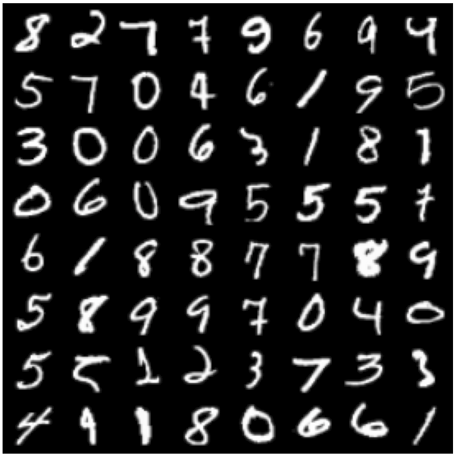
\includegraphics[width=\textwidth]{\toplevelprefix/chapters/chapter5/figs/mnist_x.png}
        \caption{MNIST $\X$}
    \end{subfigure}
    \hfill
    \begin{subfigure}[t]{0.20\textwidth}
        \centering
        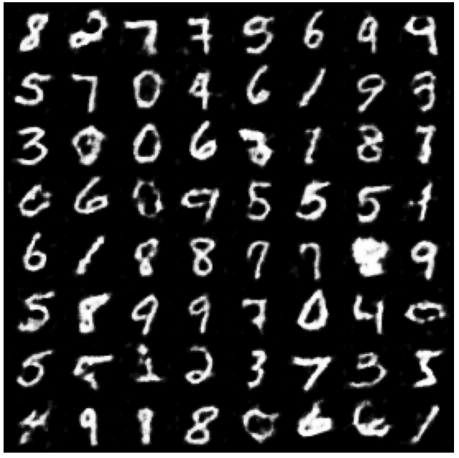
\includegraphics[width=\textwidth]{\toplevelprefix/chapters/chapter5/figs/mnist_recon_x.png}
        \caption{MNIST $\hat{\X}$}
    \end{subfigure}
    \hfill
    \begin{subfigure}[t]{0.20\textwidth}
        \centering
        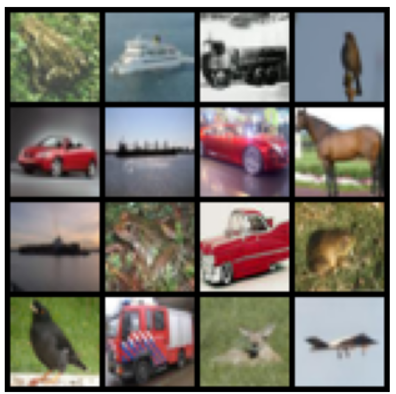
\includegraphics[width=\textwidth]{\toplevelprefix/chapters/chapter5/figs/cifar10_x.png}
        \caption{CIFAR-10 $\X$}
    \end{subfigure}
    \hfill
    \begin{subfigure}[t]{0.20\textwidth}
        \centering
        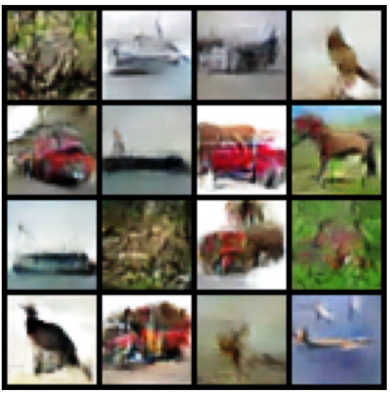
\includegraphics[width=\textwidth]{\toplevelprefix/chapters/chapter5/figs/cifar10_x_recon.png}
        \caption{CIFAR-10 $\hat{\X}$}
    \end{subfigure}
    \caption{\small Vizualizarea proprietății de auto-codare a celei învățate ($\hat{\X} = g\circ f(\X)$). }
        \label{fig:justify_xhat_equals_x_incremental}
\end{figure}


\paragraph{Subspațiile principale ale caracteristicilor învățate.}
Majoritatea metodelor generative bazate pe memorie utilizează autocodoare, VAE-uri sau GAN-uri în scopuri de redare. Structura sau distribuția caracteristicilor învățate $\Z_j$ pentru fiecare clasă este neclară în spațiul caracteristic. Caracteristicile $\Z_j$ ale memoriei LDR, pe de altă parte, au o structură liniară clară. \Cref{fig:cifar_10_pca_sampling_main} vizualizează corelațiile dintre toate caracteristicile învățate $|\Z^\top\Z|$, în care observăm modele bloc-diagonale clare pentru ambele seturi de date.\footnote{Observați că aceste modele seamănă foarte mult cu matricea de similaritate a profilurilor de răspuns ale categoriilor de obiecte din diferite zone ale cortexului inferotemporal, așa cum este arătat în Extended DataFig.3 din \cite{Bao2020AMO}.} Aceasta indică faptul că caracteristicile pentru diferite clase $\Z_j$ se află într-adevăr pe subspații care sunt incoerente unul de celălalt. Prin urmare, caracteristicile fiecărei clase pot fi bine modelate ca un subspațiu principal în spațiul caracteristic.

\begin{figure}[tb]
\centering
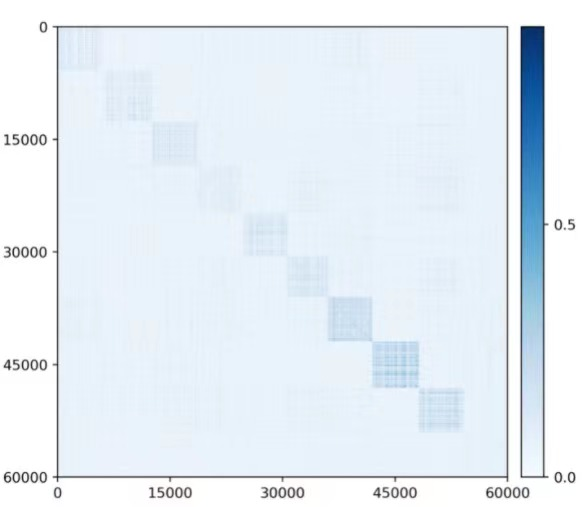
\includegraphics[height=4.1cm]{\toplevelprefix/chapters/chapter5/figs/Heatmap_MNIST.jpg}
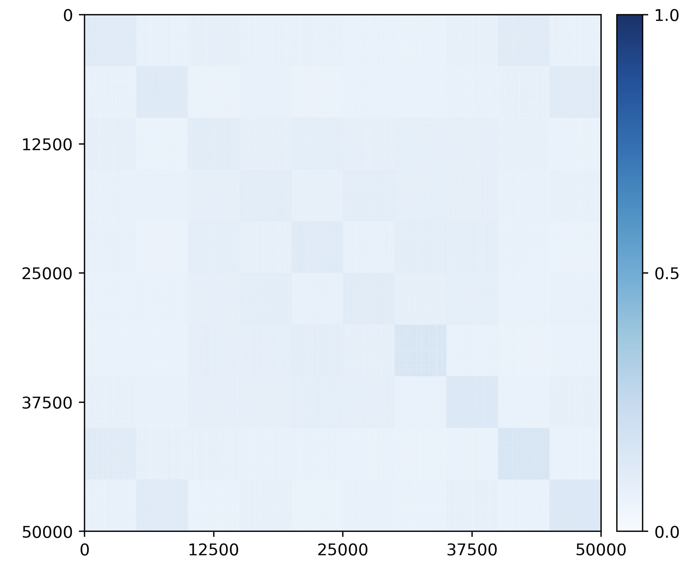
\includegraphics[height=4cm]{\toplevelprefix/chapters/chapter5/figs/Heatmap_CIFAR10.png}
\caption{\small Structura bloc diagonală a $|\Z^\top \Z|$ în spațiul caracteristic pentru MNIST (stânga) și CIFAR-10 (dreapta).}
\label{fig:cifar_10_pca_sampling_main}
\end{figure}



\paragraph{Imaginile redate ale eșantioanelor din componentele principale.}
Deoarece caracteristicile fiecărei clase pot fi modelate ca un subspațiu principal, vizualizăm în continuare componentele principale individuale din cadrul fiecăruia dintre aceste subspații. \Cref{fig:pca_sampling_main} arată imaginile redate din caracteristicile eșantionate de-a lungul primelor 4 componente principale pentru diferite clase, pe MNIST și CIFAR-10, respectiv. Fiecare rând reprezintă eșantioane de-a lungul unei componente principale și arată clar caracteristici vizuale similare, dar sunt distinct diferite de cele din alte rânduri. Vedem că modelul își amintește diferite poziții ale lui „4" după ce a învățat toate clasele rămase. Pentru CIFAR-10, memoria învățată incremental își amintește poziții și forme reprezentative ale cailor și navelor.

\begin{figure}[t]
    \begin{subfigure}[t]{0.20\textwidth}
        \centering
        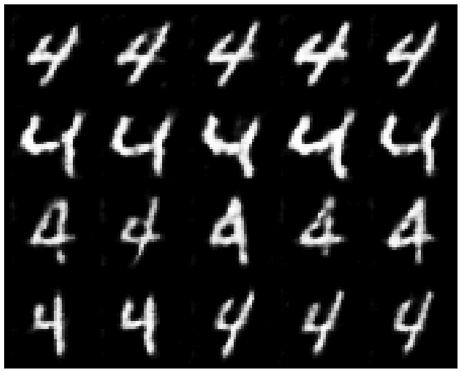
\includegraphics[width=\textwidth]{\toplevelprefix/chapters/chapter5/figs/mnist_4.png}
        \caption{$\hat{\x}_{old}$ eșantionat pentru „4"}
    \end{subfigure}
    \hfill
    \begin{subfigure}[t]{0.20\textwidth}
        \centering
        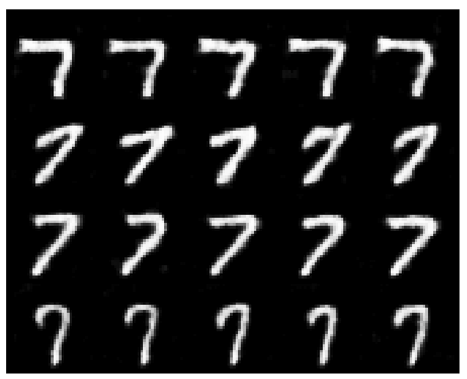
\includegraphics[width=\textwidth]{\toplevelprefix/chapters/chapter5/figs/mnist_7.png}
        \caption{$\hat{\x}_{old}$ eșantionat pentru „7"}
    \end{subfigure}
    \hfill
    \begin{subfigure}[t]{0.20\textwidth}
        \centering
        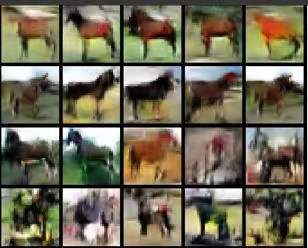
\includegraphics[width=\textwidth]{\toplevelprefix/chapters/chapter5/figs/horse_z.jpg}
        \caption{$\hat{\x}_{old}$ eșantionat pentru „cal"}
    \end{subfigure}
    \hfill
    \begin{subfigure}[t]{0.20\textwidth}
        \centering
        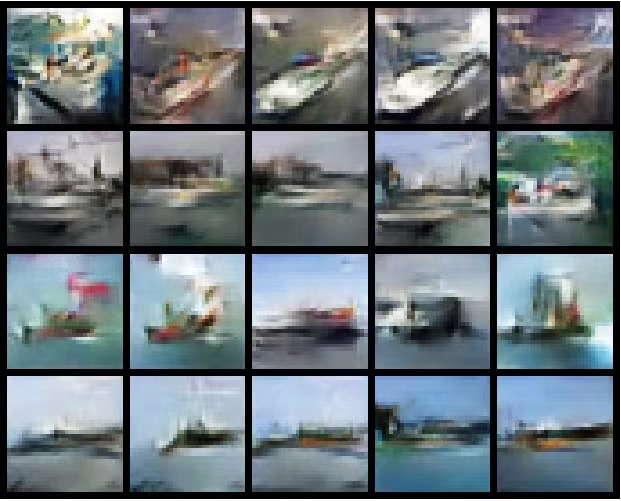
\includegraphics[width=\textwidth]{\toplevelprefix/chapters/chapter5/figs/ship_z.jpg}
        \caption{$\hat{\x}_{old}$ eșantionat pentru „navă"}
    \end{subfigure}
    \caption{\small Vizualizarea a 5 $\hat \x=g(\z)$ reconstruite din $\z$-uri cu cea mai mică distanță față de componentele principale (primele 4) ale caracteristicilor învățate pentru {MNIST} (clasa „4" și clasa „7") și {CIFAR-10} (clasa „cal" și clasa „navă").}
    \label{fig:pca_sampling_main}
\end{figure}



\paragraph{Eficacitatea revizuirii incrementale.}
Verificăm cum memoria LDR învățată incremental poate fi consolidată în continuare cu o fază de revizuire incrementală nesupravegheată descrisă anterior. Experimentele sunt efectuate pe CIFAR-10, cu 10 pași. \Cref{fig:memory_review} stânga arată imagini redate ale primei clase „avion" la sfârșitul învățării incrementale a tuturor celor zece clase, eșantionate de-a lungul primelor 3 componente principale -- fiecare două rânduri (16 imagini) sunt de-a lungul unei direcții principale. Calitatea lor vizuală rămâne foarte decentă—observăm aproape nicio uitare. Figura din dreapta arată imagini redate după revizuirea primei clase o dată. Observăm o îmbunătățire semnificativă a calității vizuale după revizuire, iar componentele principale ale caracteristicilor din subspațiu încep să corespundă atributelor vizuale distinct diferite din aceeași clasă.

\begin{figure}
\centering
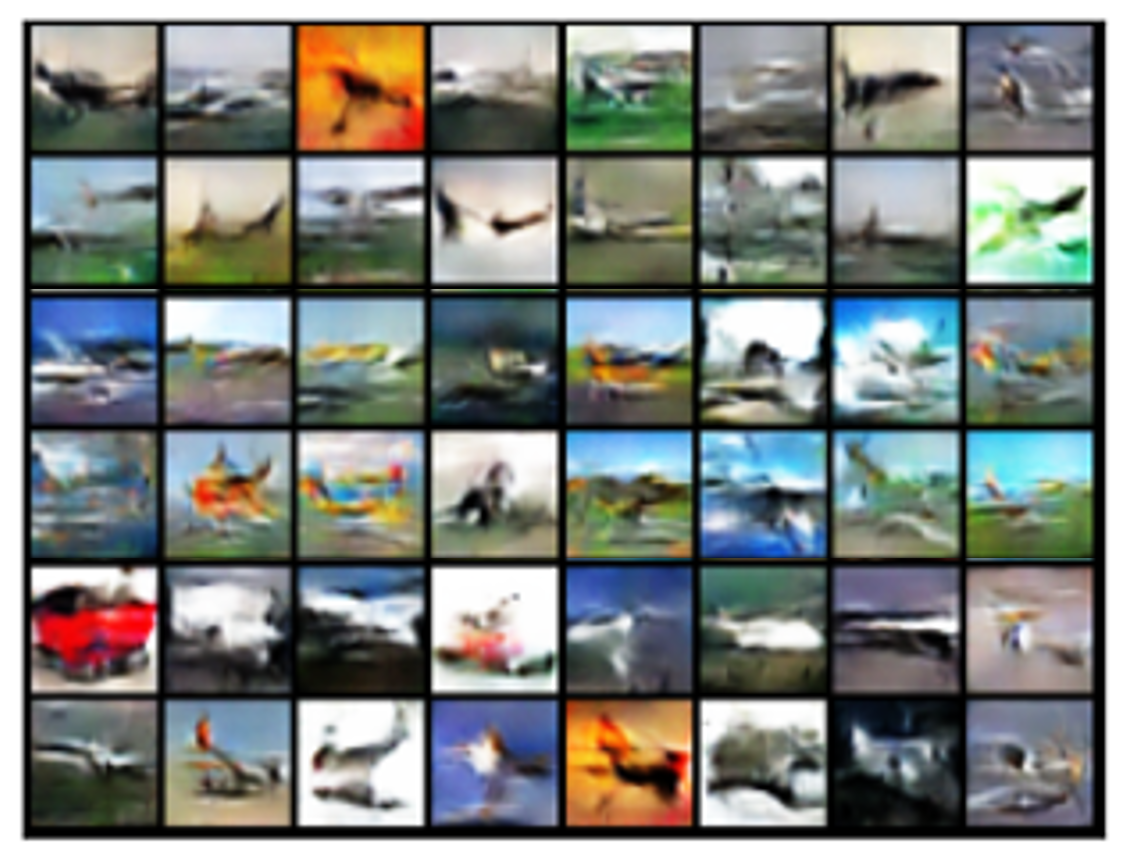
\includegraphics[width=0.41\textwidth]{\toplevelprefix/chapters/chapter5/figs/memory_before_review_clip.png}
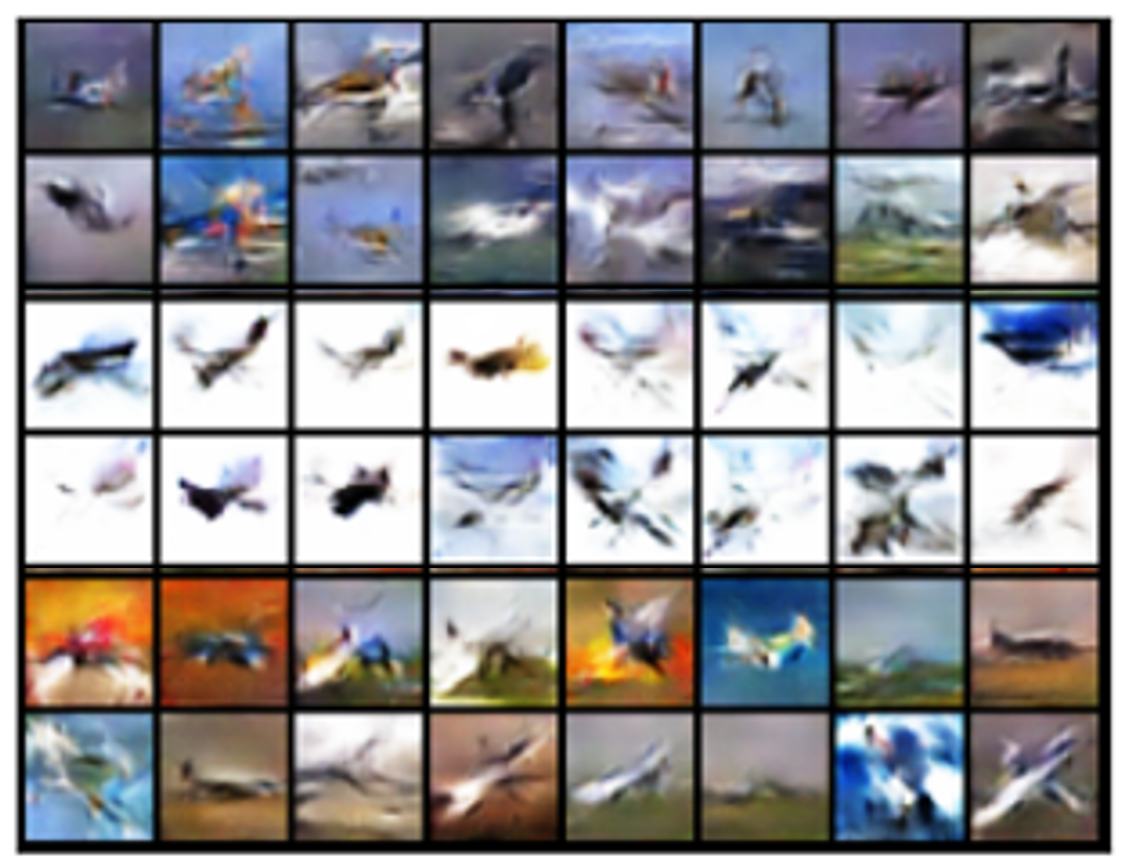
\includegraphics[width=0.4\textwidth]{\toplevelprefix/chapters/chapter5/figs/memory_after_review_clip.png}
 \caption{\small Vizualizarea imaginilor redate $\hat{\x}_{old}$ ale clasei 1-„avion" în CIFAR-10, înainte (stânga) și după (dreapta) un ciclu de revizuire.}
\label{fig:memory_review}
\end{figure}


\subsection{Învățare Nesupravegheată Continuă pe Eșantioane}
\label{sec:sample-wise-incremental}

După cum știm, formularea CTRL în buclă închisă poate învăța deja o autocodare decentă, chiar și fără informații despre clase, cu programul CTRL-Binary:
\begin{align}
      \max_{\bm \theta} \min_{\bm \eta} \quad \Delta R_\epsilon(\Z, \hat{\Z})
 \label{eqn:CTRL-Binary}
\end{align}
Cu toate acestea, observați că \eqref{eqn:CTRL-Binary} este practic limitată deoarece aliniază doar setul de date $\X$ și $\hat \X$ regenerat la nivel de distribuție.
Nu există nicio garanție că fiecare eșantion $\x$ ar fi aproape de $\hat \x = g(f(\x))$ decodat.

\paragraph{Constrângeri pe eșantioane pentru transcrierea nesupravegheată.}
\label{sec:constraints}
Pentru a îmbunătăți proprietățile discriminative și generative ale reprezentărilor învățate în cadrul nesupravegheat, propunem două mecanisme suplimentare pentru jocul maximin CTRL-Binary de mai sus \eqref{eqn:CTRL-Binary}. Pentru simplitate și uniformitate, aici acestea vor fi formulate ca constrângeri de egalitate asupra măsurilor de reducere a ratei, dar în practică ele pot fi impuse ușor în timpul optimizării.

\paragraph{Auto-consistență pe eșantioane prin transcriere în buclă închisă.}
În primul rând, pentru a aborda problema că CTRL-Binary nu învață o autocodare consistentă pe eșantioane, trebuie să promovăm ca $\hat \x$ să fie aproape de $\x$ pentru fiecare eșantion. În cadrul CTRL, acest lucru poate fi realizat prin impunerea ca caracteristicile lor corespunzătoare $\z=f(\x)$ și $\hat \z = f(\hat \x)$ să fie apropiate.
Pentru a promova auto-consistența pe eșantioane, unde $\hat{\x} = g(f(\x))$ este aproape de $\x$, vrem ca distanța dintre $\z$ și $\hat{\z}$ să fie zero sau mică, pentru toate cele $N$ eșantioane.
Această distanță poate fi măsurată prin reducerea ratei:
\begin{align}
\sum_{i\in N} \Delta R_\epsilon(\z^i,\hat{\z}^i) = 0.
\label{eqn:sample-self-consistency}\vspace{-2mm}
\end{align}
Observați că aceasta evită din nou măsurarea diferențelor în spațiul imaginii.

\paragraph{Auto-supervizare prin comprimarea eșantioanelor augmentate.}
Deoarece nu cunoaștem nicio informație despre eticheta clasei între eșantioane în cadrul nesupravegheat, cel mai bun lucru pe care îl putem face este să vedem fiecare eșantion și augmentările sale (să zicem prin translație, rotație, ocluzie etc.) ca o „clasă"—o idee de bază din spatele aproape tuturor metodelor de învățare auto-supervizată. În cadrul reducerii ratei, este natural să comprimăm caracteristicile fiecărui eșantion și augmentările sale. În această lucrare, adoptăm transformările standard din SimCLR \cite{chen2020simple} și denotăm o astfel de transformare ca $\tau$. Denotăm fiecare eșantion augmentat $\x_a = \tau(\x)$ și caracteristica sa corespunzătoare ca $\z_a = f(\x_a, \bm \theta) $. În scopuri discriminative, sperăm că clasificatorul este {\em invariant} la astfel de transformări. Prin urmare, este natural să impunem ca caracteristicile $\z_a$ ale tuturor augmentărilor să fie aceleași cu cele $\z$ ale eșantionului original $\x$. Aceasta este echivalentă cu a cere ca distanța dintre $\z$ și $\z_a$, măsurată din nou în termenii reducerii ratei, să fie zero (sau mică) pentru toate cele $N$ eșantioane:
\begin{align}
\sum_{i\in N} \Delta R_\epsilon(\z^i,\z_{a}^i) = 0.
\label{eqn:sample-compression}\vspace{-3mm}
\end{align}


\paragraph{Învățarea reprezentărilor nesupravegheate prin transcriere în buclă închisă.}
Până acum, știm că obiectivul CTRL-Binary $\Delta R_\epsilon(\Z, \hat{\Z})$ din \eqref{eqn:CTRL-Binary} ajută la alinierea distribuțiilor în timp ce auto-consistența pe eșantioane \eqref{eqn:sample-self-consistency} și augmentarea pe eșantioane \eqref{eqn:sample-compression} ajută la alinierea și comprimarea caracteristicilor asociate cu fiecare eșantion. Pe lângă consistență, vrem, de asemenea, ca reprezentările învățate să fie maxim discriminative pentru diferite eșantioane (aici văzute ca diferite „clase"). Observați că termenul de distorsiune a ratei $R_\epsilon(\Z)$ măsoară rata de codare (deci volumul) tuturor caracteristicilor.

\paragraph{CTRL nesupravegheat.} Punând aceste elemente împreună, propunem să învățăm o reprezentare prin următorul program maximin constrâns, pe care îl numim {\em CTRL nesupravegheat} (u-CTRL):
\begin{align}
      \max_\theta \min_\eta  \quad & R_\epsilon(\Z) + \Delta R_\epsilon(\Z, \hat{\Z}) \label{eqn:constrained_maxmin}\\
 \mbox{supus la} \quad & \sum_{i\in N} \Delta R_\epsilon(\z^i, \hat{\z}^i) = 0, \;\; \mbox{și} \;\; \sum_{i\in N} \Delta R_\epsilon(\z^i, \z_{a}^i) = 0. \nonumber
\end{align}
\Cref{fig:framework-uCTRL} ilustrează arhitectura generală a sistemului în buclă închisă asociat cu acest program.
\begin{figure}[t]
\centering
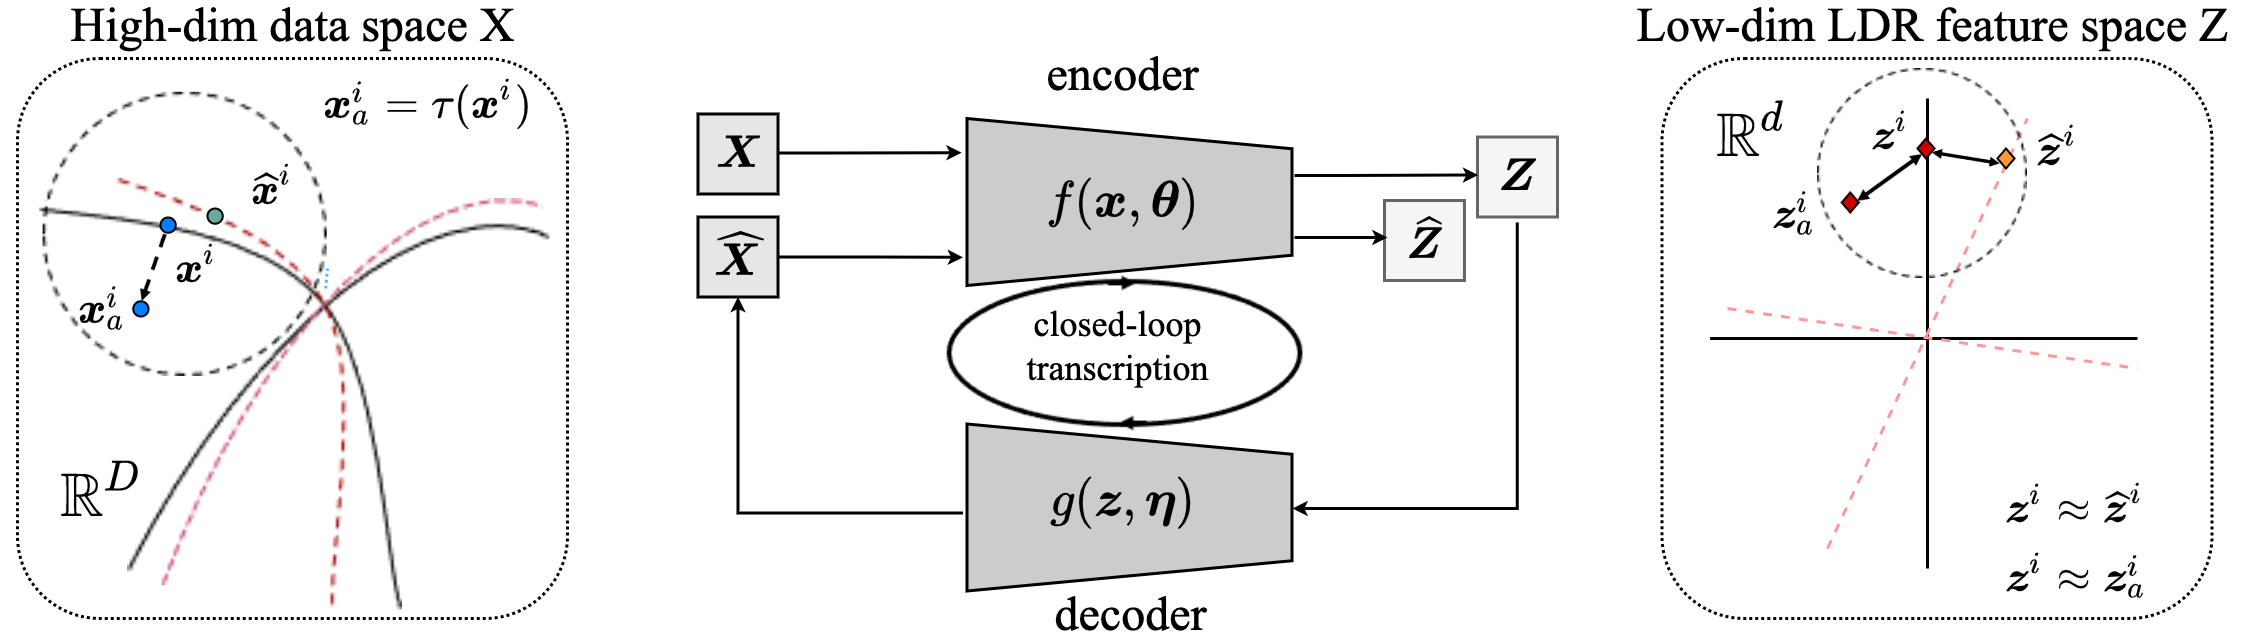
\includegraphics[width=0.98\textwidth]{\toplevelprefix/chapters/chapter5/figs/uCTRLv3.png}
\caption{\textbf{Cadrul general} al transcrierii în buclă închisă pentru învățarea nesupravegheată. Două constrângeri suplimentare sunt impuse asupra metodei Binary-CTRL: 1) auto-consistență pentru caracteristicile pe eșantioane $\z^i$ și $\hat{\z}^i$, să zicem $\z^i \approx \hat{\z}^i$; și 2) invarianță/similaritate între caracteristicile eșantioanelor augmentate $\z^i$ și $\z_{a}^i$, să zicem $\z^i \approx \z_{a}^i=f(\tau(\x^i), \bm \theta)$, unde $\x^i_a=\tau(\x^i)$ este o augmentare a eșantionului $\x^i$ prin o anumită transformare $\tau(\cdot)$.}
\label{fig:framework-uCTRL}
\end{figure}

În practică, programul de mai sus poate fi optimizat prin maximizare și minimizare alternativă între codificatorul $f(\cdot,\bm \theta)$ și decodificatorul $g(\cdot,\bm \eta)$. Adoptăm următoarea strategie de optimizare care funcționează bine în practică, care este folosită pentru toate experimentele ulterioare pe seturi de date de imagini reale:
\vspace{-1mm}
\begin{align}
  &  \max_{\theta}\; R_\epsilon(\Z) + \Delta{R_\epsilon(\Z, \hat{\Z})-\lambda_{1}\sum_{i\in N} \Delta R_\epsilon(\z^i, \z_{a}^i)} -\lambda_{2}\sum_{i\in N} \Delta R_\epsilon(\z^i, \hat{\z}^i) \label{eqn:constrained_max}; \\
   & \min_{\eta}\; R_\epsilon(\Z) + \Delta{R_\epsilon(\Z, \hat{\Z})+\lambda_{1}\sum_{i\in N} \Delta R_\epsilon(\z^i, \z_{a}^i)+ \lambda_{2}\sum_{i\in N} \Delta R_\epsilon(\z^i, \hat{\z}^i)} \label{eqn:constrained_min},
\end{align}
unde constrângerile $\sum_{i\in N} \Delta R_\epsilon(\z^i, \hat{\z}^i) = 0$ și $\sum_{i\in N} \Delta R_\epsilon(\z^i, \z_{a}^i) = 0$ din \eqref{eqn:constrained_maxmin} au fost convertite (și relaxate) în termeni Lagrangieni cu coeficienții corespunzători $\lambda_{1}$ și $\lambda_{2}$.\footnote{Observați că calcularea termenilor de reducere a ratei $\Delta R$ pentru toate eșantioanele sau un lot de eșantioane necesită calcularea costisitoare a $\log\det$ a matricelor mari. În practică, din semnificația geometrică a $\Delta R$ pentru doi vectori, $\Delta R$ poate fi aproximat cu o normă $\ell^2$ sau distanța cosinus între doi vectori.}

Reprezentarea de mai sus este învățată fără informații despre clase. Pentru a facilita sarcinile discriminative sau generative, aceasta trebuie să fie foarte structurată. S-a verificat experimental că acesta este într-adevăr cazul și u-CTRL demonstrează avantaje semnificative față de alte metode de învățare incrementală sau nesupravegheată \cite{pmlr-v234-tong24a}. Aici ilustrăm doar câteva rezultate calitative cu experimentul pe setul de date CIFAR-10 \cite{krizhevsky2014cifar}, cu augmentări standard pentru învățarea auto-supervizată \cite{chen2020simple}. Se poate consulta \cite{pmlr-v234-tong24a} pentru experimente pe seturi de date mai multe și mai mari și evaluările lor cantitative.

După cum se poate vedea din experimente, o structură specifică și unică apare într-adevăr în mod natural în reprezentările învățate folosind u-CTRL: global, caracteristicile imaginilor din aceeași clasă tind să fie grupate bine împreună și separate de alte clase, așa cum este arătat în \Cref{fig:heatmap_z}; local, caracteristicile din jurul eșantioanelor individuale prezintă structuri aproximativ liniare pe bucăți de dimensiune redusă, așa cum este arătat în \Cref{fig:tsne}.

\begin{figure}[t]
     \footnotesize
     \centering
    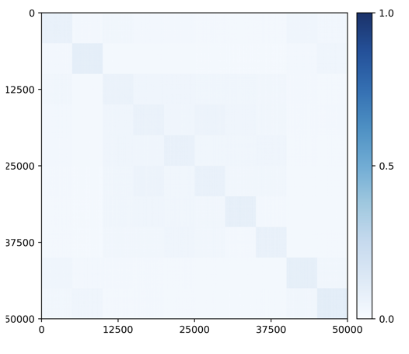
\includegraphics[width=0.5\textwidth]{\toplevelprefix/chapters/chapter5/figs/CIFAR10_cifar10_heatmap_zz.png}
    \caption{\small Apariția structurilor bloc-diagonale ale $|\Z^\top \Z|$ în spațiul caracteristic pentru CIFAR-10.}
    \label{fig:heatmap_z}
\end{figure}

\begin{figure}[ht!]
    \begin{subfigure}[t]{0.46\textwidth}
        \centering
        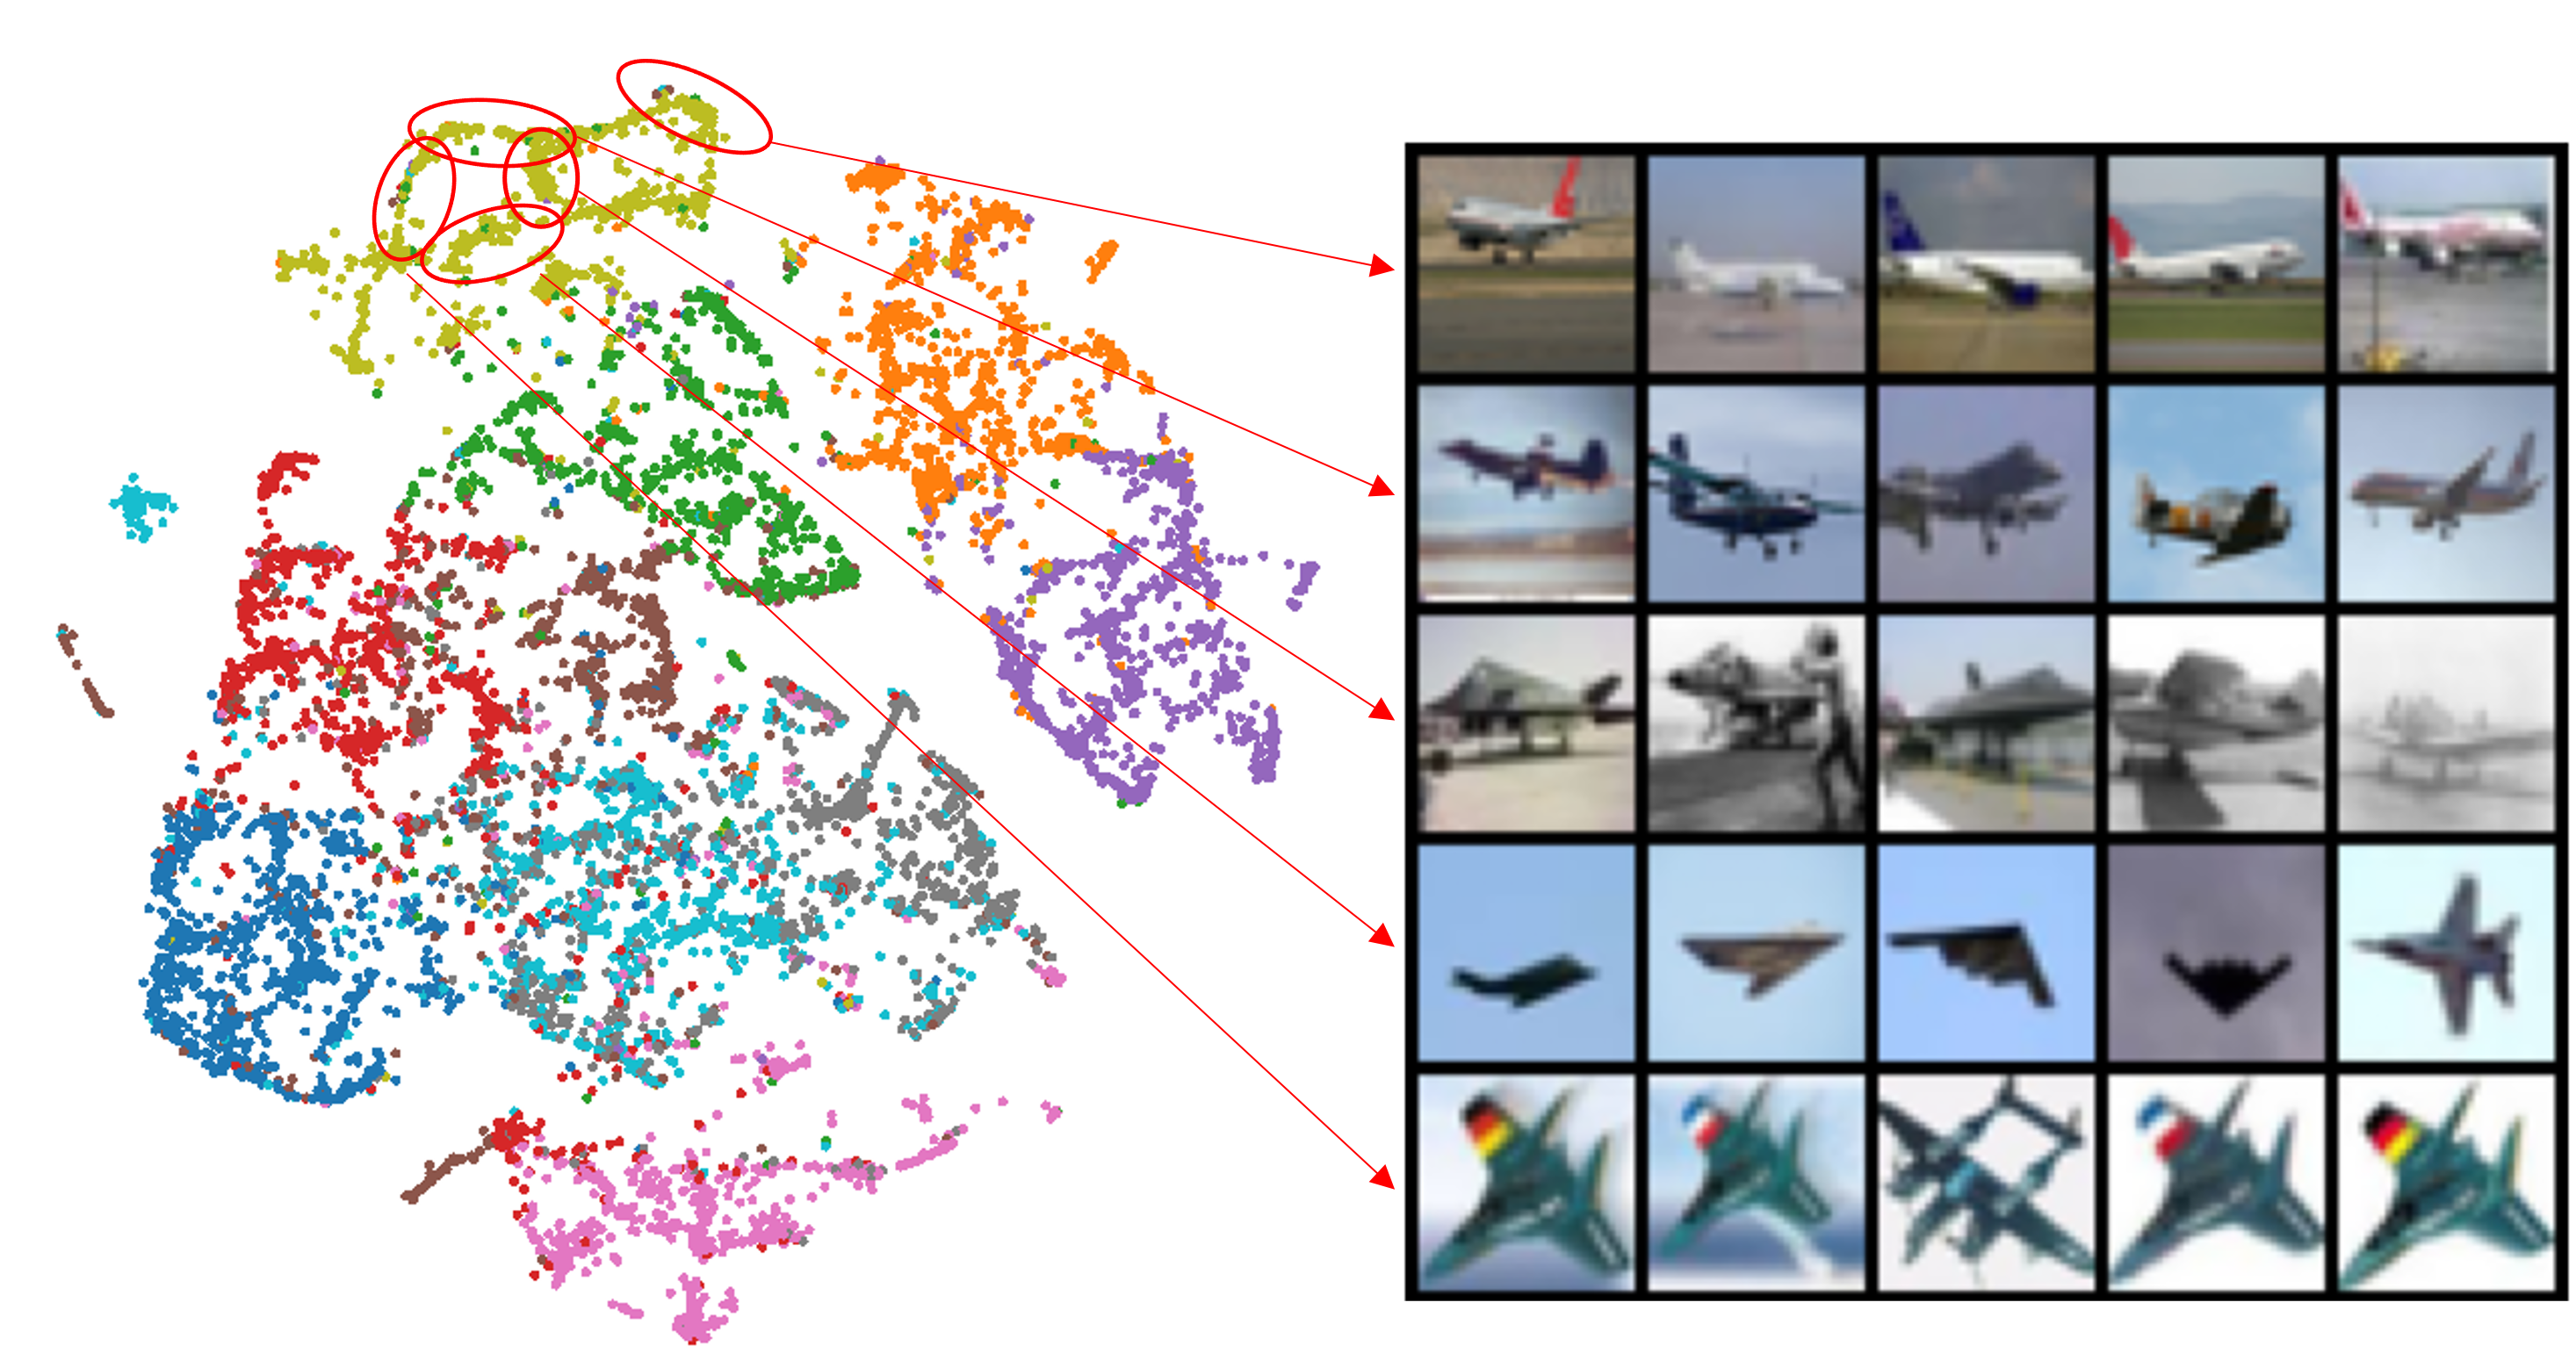
\includegraphics[width=\textwidth]{\toplevelprefix/chapters/chapter5/figs/uCTRL-tsne2.png}
        \caption{u-CTRL}
    \end{subfigure}
    \hfill
    \begin{subfigure}[t]{0.46\textwidth}
        \centering
        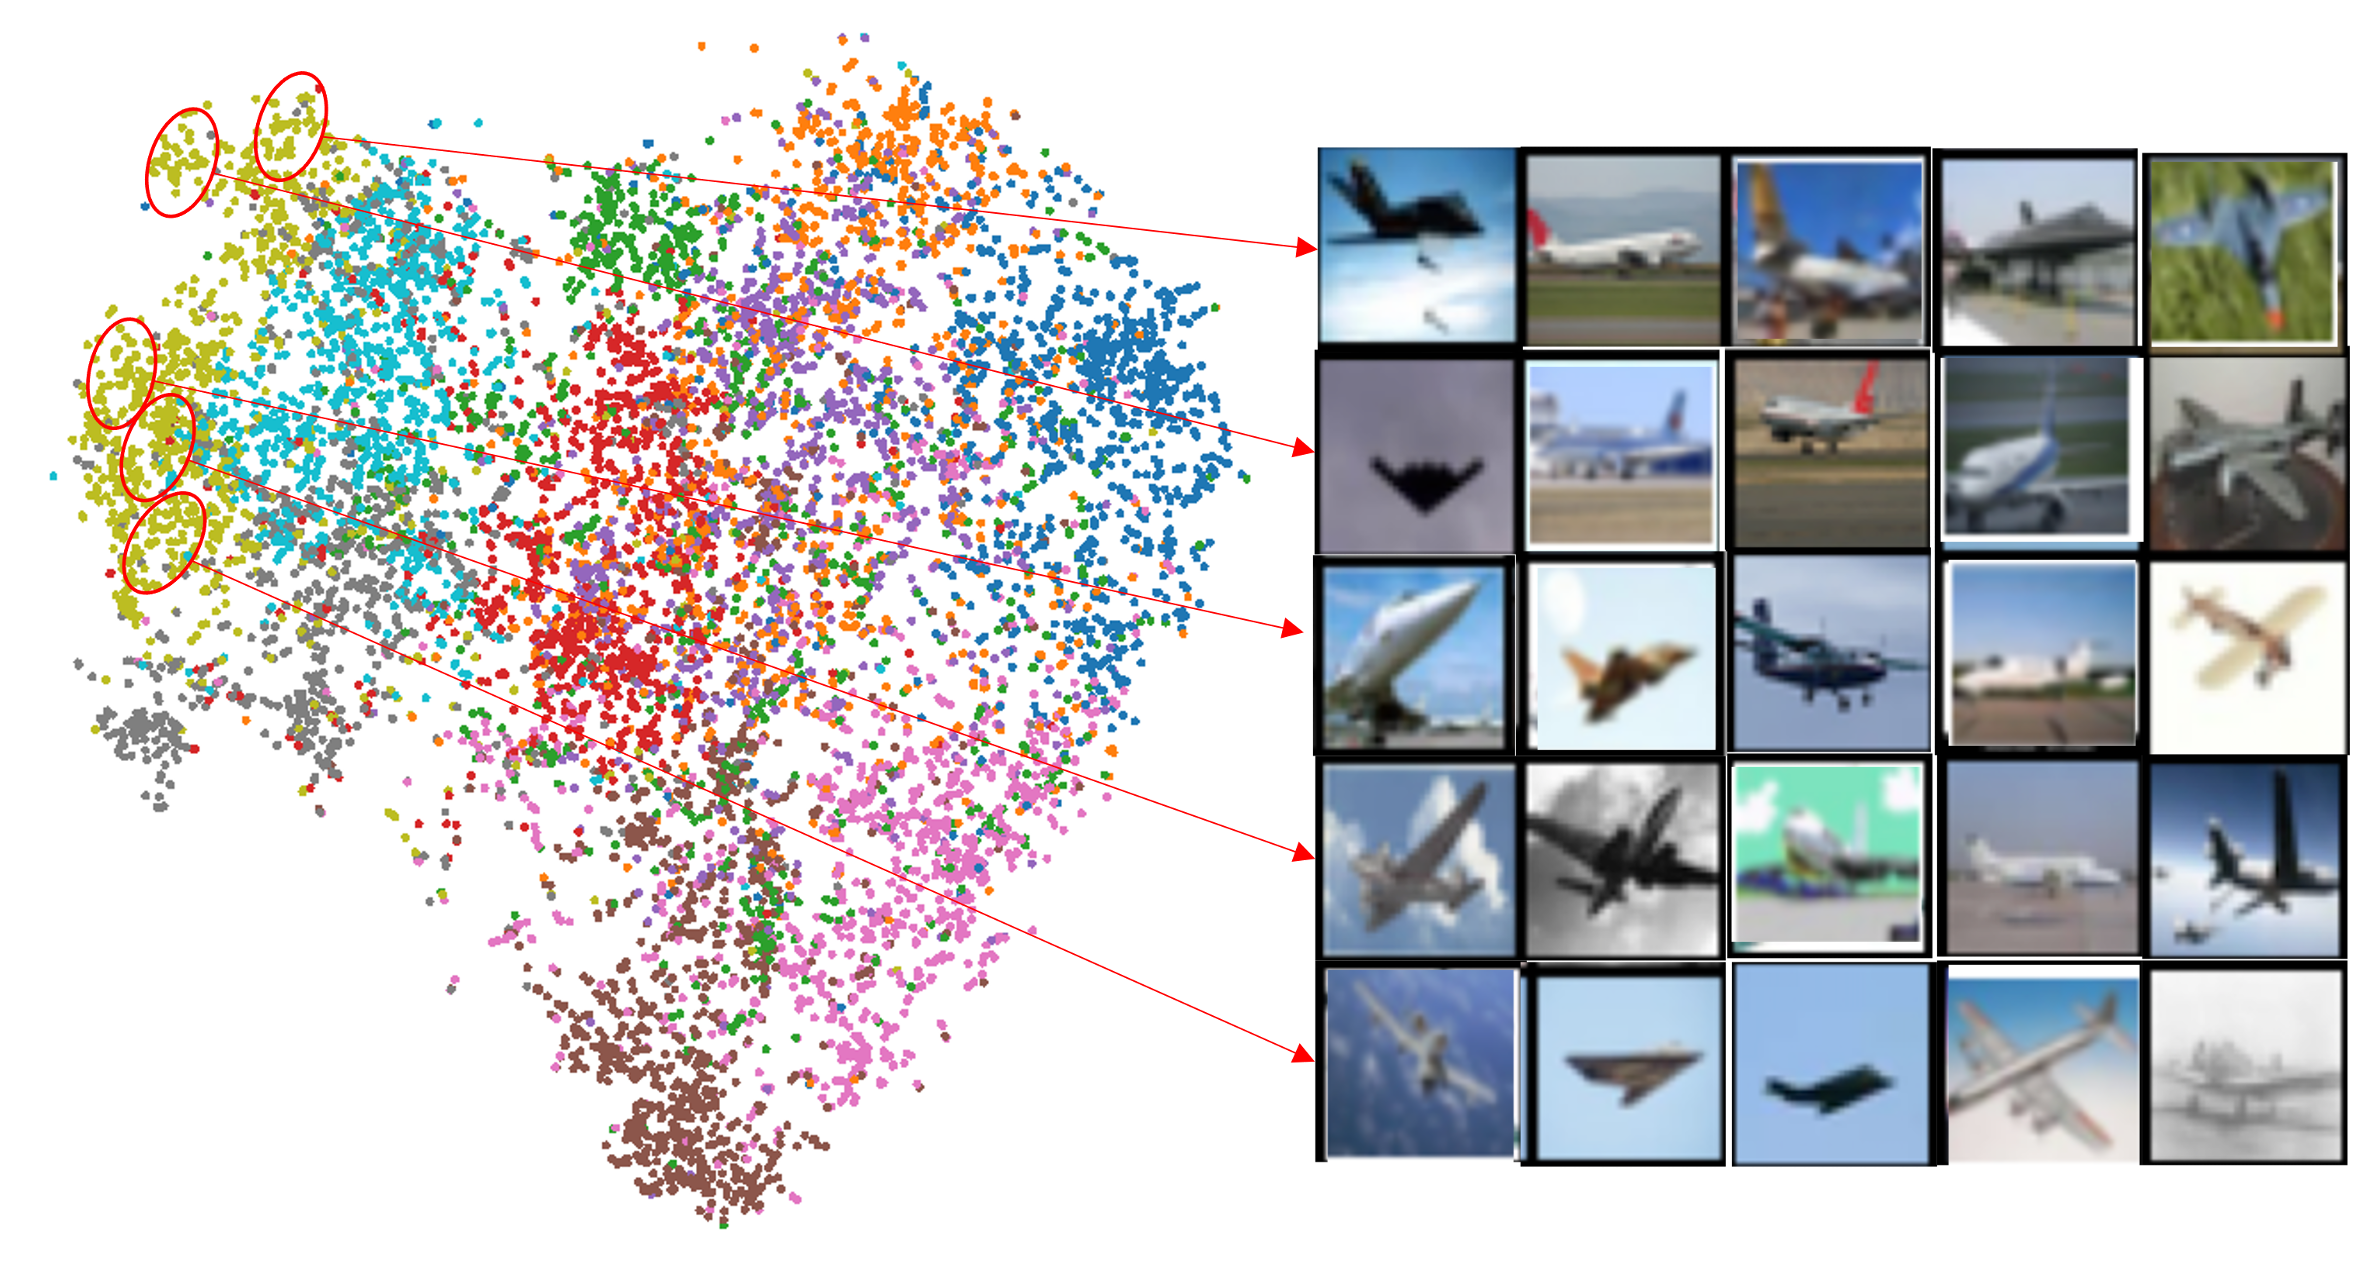
\includegraphics[width=\textwidth]{\toplevelprefix/chapters/chapter5/figs/MoCoV2-tsne3.png}
        \caption{MoCoV2}
    \end{subfigure}
    \caption{\small Vizualizări t-SNE ale caracteristicilor învățate ale CIFAR-10 cu diferite modele.}
    \label{fig:tsne}
\end{figure}

\paragraph{Generarea nesupravegheată condiționată de imagini prin reducerea ratei.}
Distribuția de caracteristici foarte structurată sugerează, de asemenea, că reprezentarea învățată poate fi foarte utilă în scopuri generative. De exemplu, putem organiza caracteristicile eșantioanelor în clustere semnificative și le putem modela cu distribuții (gaussiene) sau subspații de dimensiune redusă. Prin eșantionarea din aceste modele compacte, putem regenera condiționat eșantioane semnificative din clusterele calculate. Aceasta este cunoscută ca {\em generare nesupravegheată condiționată de imagini} \cite{hwang2021stein}.

Pentru a grupa caracteristicile, exploatăm faptul că cadrul de reducere a ratei \eqref{eqn:maximal-rate-reduction} este inspirat de gruparea nesupravegheată prin compresie \cite{ma2007segmentation}, care oferă o modalitate principială de a găsi apartenența $\bm \Pi$.
Concret, maximizăm același obiectiv de reducere a ratei \eqref{eqn:maximal-rate-reduction} peste $\bm \Pi$, dar fixăm reprezentarea învățată $\Z$ în schimb. Vedem pur și simplu apartenența $\bm \Pi$ ca o funcție neliniară a caracteristicilor $\Z$, să zicem $h_{\bm \pi}(\cdot,\xi):\Z \mapsto \bm \Pi$ cu parametrii $\xi$. În practică, modelăm această funcție cu o rețea neuronală simplă, cum ar fi un cap MLP imediat după caracteristica de ieșire $\z$.
Pentru a estima o apartenență „pseudo" $\hat{\bm \Pi}$ a eșantioanelor, rezolvăm următoarea problemă de optimizare peste $\bm \Pi$:
\begin{align}
    \hat{\bm \Pi} = \arg\max_{\xi} \Delta R_\epsilon(\Z| \bm \Pi(\xi)).
\label{eqn:cluster_mcr}
\end{align}
În \Cref{fig:vis_clustering}, vizualizăm imagini generate din cele zece clustere nesupravegheate din \eqref{eqn:cluster_mcr}. Fiecare bloc reprezintă un cluster și fiecare rând reprezintă o componentă principală pentru fiecare cluster. În ciuda învățării și antrenării fără etichete, modelul nu numai că organizează eșantioanele în clustere corecte, dar este, de asemenea, capabil să păstreze diversitățile statistice din cadrul fiecărui cluster/clasă. Putem recupera cu ușurință diversitatea din cadrul fiecărui cluster calculând diferite componente principale și apoi eșantionând și generând în consecință. Deși experimentele prezentate aici sunt oarecum limitate în scară, vom explora metode mai directe și mai puternice care utilizează distribuțiile de date și reprezentările învățate pentru generarea și estimarea condiționată în capitolul următor.
\begin{figure}[t]
    \footnotesize
    \centering
    \includegraphics[width=0.95\textwidth]{\toplevelprefix/chapters/chapter5/figs/CIFAR10_generatedfromcluster.png}
    \caption{\small Generarea nesupravegheată condiționată de imagini din fiecare cluster al CIFAR-10, folosind u-CTRL. Imaginile din rânduri diferite înseamnă generare din componente principale diferite ale fiecărui cluster.}
    \label{fig:vis_clustering}
\end{figure}





\section{Rezumat și Note}
Istoric, autocodarea a fost unul dintre factorii importanți de inovare în cercetarea
rețelelor neuronale pentru învățare, deși cele mai impresionante demonstrații practice
ale învățării profunde au fost probabil în alte domenii
(cum ar fi clasificarea discriminativă, cu AlexNet
\cite{krizhevsky2012imagenet}, sau modelarea generativă cu arhitecturi GPT
\cite{brown2020language}).
Lucrările pe care le-am prezentat pe parcursul capitolului, în special lucrarea lui
\cite{Hinton504}, au servit drept catalizatori ai interesului de cercetare în rețelele neuronale
în perioadele în care nu erau altfel proeminente în peisajul cercetării în învățarea automată.
În practica modernă, autocodoarele rămân componente de bază ale multor sisteme la scară largă
pentru generarea de date foarte structurate, cum ar fi date vizuale, date de vorbire
și date moleculare, în special abordarea VQ-VAE
\cite{van-den-Oord2017-jr}, care se bazează pe metodologia autocodorului variațional
pe care am discutat-o în \Cref{sec:vae}.
Problema de bază a autocodării rămâne de o importanță intelectuală primordială
datorită conexiunii sale strânse cu învățarea reprezentărilor și anticipăm că
va reapărea pe radarul cercetătorilor practici în viitor pe măsură ce
eficiența în antrenarea și implementarea modelelor mari continuă să devină mai
importantă.

Materialele prezentate în a doua jumătate a acestui capitol se bazează pe o serie de
lucrări recente pe tema transcrierii în buclă închisă: \cite{Dai-entropy-2022},
\cite{pai2022pursuit}, \cite{tong2023incremental} și \cite{pmlr-v234-tong24a}. În special, \Cref{sec:closed-loop-transcription} se bazează pe lucrarea pionieră a \cite{Dai-entropy-2022}. După aceea, lucrarea \cite{pai2022pursuit} a oferit justificări teoretice puternice pentru cadrul în buclă închisă, cel puțin pentru un caz ideal. \Cref{sec:class-wise-incremental} și \Cref{sec:sample-wise-incremental} se bazează pe lucrările \cite{tong2023incremental} și, respectiv, \cite{pmlr-v234-tong24a}. Ele demonstrează că cadrul în buclă închisă sprijină în mod natural învățarea incrementală și continuă, fie într-un cadru pe clase sau pe eșantioane. Cititorul poate consulta aceste lucrări pentru mai multe detalii tehnice și experimentale.


\paragraph{Rețele neuronale puțin adânci vs.\ profunde, pentru autocodare și mai mult.}
În \Cref{sub:nonlinear-pca}, am discutat teorema de aproximare universală a lui Cybenko
și cum aceasta afirmă că, în principiu, o rețea neuronală cu un singur
strat ascuns (și neliniarități elementare adecvate) este suficientă pentru
a aproxima orice funcție țintă regulară adecvat. Desigur, în practică,
motivul arhitectural major pentru dominația rețelelor neuronale în practică a fost
rafinarea tehnicilor pentru antrenarea rețelelor neuronale \textit{mai profunde}.
De ce este necesară profunzimea?
Din punct de vedere fundamental, problema separărilor de profunzime, care
construiește setări în care o rețea neuronală mai profundă poate aproxima o clasă dată
de funcții țintă cu eficiență exponențial superioară față de o rețea
puțin adâncă,
a fost studiată pe larg în literatura teoretică:
exemplele includ \cite{Telgarsky2016-sn,Bresler2020-xy,Venturi2021-qc}.
Ușurința antrenării rețelelor mai profunde
în practică nu a primit un răspuns la fel de satisfăcător din
perspectiva teoriei.
ResNet-urile \cite{he2016deep} reprezintă lucrarea empirică pionieră de
a face rețelele mai profunde mai ușor de antrenat, folosite în aproape toate arhitecturile
moderne într-o anumită formă. Studiile teoretice s-au concentrat foarte mult pe
antrenabilitatea rețelelor foarte profunde, cuantificată prin nucleul tangent neuronal
inițial \cite{Buchanan2021-sj,Martens2021-cx}, dar aceste studii nu au oferit
perspective semnificative asupra beneficiilor de antrenabilitate ale rețelelor mai profunde în etapele
medii și târzii ale antrenării (dar vezi \cite{Yang2021-gw} pentru rădăcina unei linii
de cercetare care încearcă să abordeze acest lucru).

\section{Exerciții și Extensii}

\begin{exercise}[Înțelegerea Conceptuală a Aplatizării Varietății]
  Considerați date care se află pe o varietate curbată $\cM$ încorporată în $\R^D$ (precum
  o suprafață curbată în spațiul tridimensional), așa cum este discutat în subsecțiunea
  aplatizării varietății din \Cref{sub:nonlinear-pca}.
  În acest exercițiu, vom descrie ingredientele de bază ale algoritmului de
  aplatizare a varietății din \cite{Psenka-JMLR24}.
  O varietate este numită plată dacă este un set deschis în spațiul euclidian (sau
  mai general, un set deschis într-un subspațiu).

  \begin{enumerate}
    \item Să presupunem că varietatea $\cM$ este un \textit{graf}: aceasta înseamnă că $\cM
      \subset \R^{D_1} \times \R^{D_2}$ (să zicem), și că există o funcție $F
      : \R^{D_1} \to \R^{D_2}$ astfel încât
      \begin{equation}
        \cM = \set{(\x, F(\x) \mid \x \in \R^{D_1})}.
      \end{equation}
      Dați un întreg $D_3$ și o hartă $f : \R^{D_1} \times \R^{D_2} \to \R^{D_3}$
      care aplatizează $\cM$ și descrieți procedura de reconstrucție corespunzătoare
      (fără pierderi) din reprezentarea aplatizată.
    \item Acum să presupunem că $\cM$ este o varietate netedă generală. Varietățile netede
      au proprietatea că sunt bine aproximate local de subspații
      în apropierea fiecărui punct. Descrieți în termeni intuitivi cum să aplatizați varietatea
      $\cM$ local la fiecare punct, prin raportarea la un graf. (Algoritmul din
      \cite{Psenka-JMLR24} efectuează o versiune rafinată a acestui proces de aplatizare
      locală într-un mod care le permite să fie lipite împreună pentru a forma o aplatizare
      globală.)
  \end{enumerate}
\end{exercise}


\begin{exercise}[Reproduceți Transcrierea în Buclă Închisă]

  Implementați o conductă de transcriere în buclă închisă pentru învățarea reprezentărilor pe
  setul de date CIFAR-10 urmând
  metodologia din \Cref{sec:closed-loop-transcription}.
  Consultați \cite{Dai-entropy-2022} pentru hiperparametri utili și setări de
  arhitectură. Reproduceți rezultatul din \Cref{fig:justifyz=z}.


\end{exercise}

\end{document}
